\documentclass[twocolumn,aps,sort,nofootinbib]{revtex4}
%\documentclass[twocolumn,aps,sort,numerical,reprint]{revtex4}
\usepackage{amssymb,amsmath,amsthm}
\usepackage{graphicx}
\usepackage{color}
\usepackage{epic}
\usepackage{appendix}
\usepackage[caption=false]{subfig}
\usepackage[linktocpage=true,hyperindex=true,colorlinks=true]{hyperref}
\usepackage{tikz}
\usepackage{bbm}
%%%%%%
\newtheorem{theorem}{Theorem}[section]
\newtheorem{lema}{Lema}[section]
\newtheorem{corolary}{Corolary}[section]
\newtheorem{question}{Q}
\newtheorem{definition}{Definition}
\newtheorem{conjecture}{Conjecture}
\newcommand{\link}[2][url]{\href{#2}{#1}}

\begin{document}
\title{On the role of Symmetry in the Community-Finding Problem in
Complex Networks: Statistical Mechanics of clustering}
\author{Miguel A. Santos}
\affiliation{Centre for Computational Biology, The Hospital for Sick Children,
555 University Avenue,Toronto, Ontario, M5G 1X8}
\begin{abstract}
This text represents the personal notes of the author on
a work in progress.
We describe the role of symmetry in the problem of finding communities in
a complex network. We outline a possible matrix representation of
partitions that carries a geometric interpretation as rotations in a
space of $N$ dimensions.
We discuss the possibility of re-defining 
Zurek's algorithmic distance measure such that
it takes into account the {\em a priori} information
defining the clustering problem.
This leads us to outline a general theoretical approach 
for identifying clusters among 
a set of elements in a way that is analogous to the MaxEntropy approach of 
Statistical Mechanics. The graph of pairwise affinities %(dis)similarities
between elements is the basic input. Fixing the
appropriate averages should determine the corresponding optimal clustering.
\end{abstract}


\email{msantos@wodaklab.org}
\homepage{http://wodaklab.org}
\date{\today}
\maketitle
\tableofcontents

%%%%%%%%%%%%%%%%%%%%%%
\section{Introduction}
\subsection{Overview}
Since the seminal works of Strogatz and Watts \cite{Strogatz98},
Barab\'asi and Albert \cite{Barabasi99} and that of 
Girvan and Newman \cite{Girvan02}, complex networks in general,
but in particular
the community finding problem is being devoted 
a constantly increasing interested within the
fields of Physics and Mathematics \cite{Fortunato10,Evans10,Porter09}.
However, many other fields sparked the
initial interest in these topics, albeit disguised under
different names.  
Indeed, clustering a set of objects into disjoint classes is
an ubiquitous step in many problems across a variety
of other fields, from Engineering and Computer Science
(communication and information networks, database systems, 
information retrieval), to Biology, Sociology 
(biological and social networks)
and
%Information Retrieval and Automated Speech Recognition 
Computational Linguistics
\cite{Schaeffer07,Griffiths86,ICTIR2009,Justo05,Clark01}. 
In some
sense, it can be regarded as one basic learning
skill: Identifying two or more distinct groups across  
an initial set of seemingly identical 
(or completely different) 
objects leads
the way to investigate further details of each group.
This view somehow encompasses the idea of emergent phenomena
typical of complex systems.
%%Incidentally, that is the etymological meaning of the
%%word \textit{analysis}. 
%% The importance of this
%% concept was appropriately identified long time ago
%% by the community of Artificial Intelligence (AI): 
In computer science, more often than not clustering algorithms
are found under the heading of (un)supervised \textit{learning} 
algorithms, thereby explicitly highlighting its conceptual relevance. 
Furthermore, the concept itself of 
a partition may play a key role in analyzing different
problems, even if their study do not involve an	 
explicit clustering step. Particular examples of problems
involving these concepts include drug discovery, in
Chemistry; function determination of proteins
based on their sequences, in Bioinformatics; optimal design of
integrated circuits, in Engineering; the study of 
fragmentation processes in Nuclear and Condensed Matter Physics; 
first-order phase transitions in ferromagnetic materials; (bla,bla,bla).
(NEEDS EXAMPLES/REFERENCES!!)

Each field has its own particular nuances leading to such
a clustering problem. 
In Biology, it is a tacitly accepted principle that, in general, a
protein sequence determines its function. This statement itself bears 
some additional difficulties as there is no definite consensus
on what is meant by function. For instance, it could be understood at 
a molecular level, e.g. binding to DNA, 
at a metabolic level, affecting a chain of reactions, or
at a phenotypic level. Despite such an issue, it is
widely assumed that, considering also Anfinsen's dogma, all the information
of the 3-dimensional structure and function of a protein is
coded into
its sequence (see \cite{BenNaim11} and references therein for a recent dispute of it). 
A fundamental problem in Bioinformatics is then to determine 
a protein's function from its sequence. The most common approach is
finding an answer by comparison against a set of similar (homologous) proteins for 
which their function is known. 
A variant of this problem, however, is to determine subfamilies of 
slightly different specificities among a set of proteins with a common
generic function. This is a clustering problem for which one can
find almost as many different procedures as published articles about it,
each considering the different additional information or algorithmic approaches
the authors may consider fit.
%In particular here exists a wealth of different clustering algorithms but, 

Independently of the validity of the biological assumptions leading to such
a clustering problem, the latter may still be of relevance, as one 
may ask about the amount of information on a protein's function one
may extract from its sequence, even if function is not {\sl uniquely} determined
by the protein sequence {\sl alone}. A clear formulation of the clustering
problem and its solution may offer a solid ground upon which such question
could be clarified. A similar conclusion may be drawn in other fields
as well. Therefore, we will not further question the validity
of the clustering problem, but assumed it as given.

Usually,
the particular method used to solve a clustering problem
depends on the details of
the problem under study as well as on idiosyncratic 
preferences of the community or authors involved. In general,
in the approaches hitherto found in the literature,
the number of free parameters used is
usually arbitrary and these lack a sound rationale for
their inclusion; rather, they are justified {\sl a posteriori}
as those free parameters that allow one to obtain a 
pre-defined solution\cite{Schaeffer07}. 
(MORE EXAMPLES/REFERENCES?? ). 
({\sl DOUBLECHECK: 
However, two general approaches, 
MCL \cite{MCL} and Affinity Propagation \cite{AffinityPropagation}, 
deserve
a special mention. Affinity Propagation may
have a sound formulation as a 
belief propagation minimizing the distance to a centroid,
but its description lacks an easy intuitive
view of the parameters 
used and their relevance in obtaining  the optimal partition.
Analogously, MCL, while similar in spirit -optimizing a markov flow
on the network- does not really output an optimal clustering
solution, as it lacks a scoring function to compare solutions against
each other, but rather represents just a fast algorithm for sampling
the partition space.})
Thus, to a large
extent, the program set out in \cite{Lance67-1,Lance67-2} is seen as
a reference yet: They all solve the {\sl computational} problem of 
devising, by any reasonable means, an empirical method for
classifying the given data\cite{Lance67-2}.
%finding a solution {\sl here and now} by any reasonable means.

\begin{figure}
\centering
\includegraphics[width=0.5\textwidth]{Figures/CommunityDetection-network-weighted-3.jpg}
\caption{The problem of clustering in a weighted network. 
%% We can distinguish three types of clustering problems: 
%% connectivity-based system, bond-robustness and that of an
%% attraction-repulsion system. The latter is described in
%% Fig.(\ref{BayesianDistanceMeasure}) while the other two
%% are discribed next.
The weights are assumed given by a pairwise matrix $\boldsymbol{\omega}$,
called the {\sl affinity} matrix, and may have varying meanings.
Different edge weights
are denoted by different edge widths.
Edges are $1,2,3,4,8$ and $12$ pixels in width.
The vertices can be grouped into different clusters or communities
depending on the criteria and information used.
The spatial distribution of connectivities and vertices may easily
lead the eye to distinguish the $3$ clusters sketched. 
A topological criterion based solely on the connectivities of 
the vertices may be used in a computer program to 
identify the same three clusters by way of
removing the edges with highest betweenness. 
However, a different algorithm that would consider
the edge width as a kind of {\em bond strength}
might well yield just $2$ clusters:
the $12$px width edge, joining two of the former
clusters, might be strong enough to consider both groups 
together as the optimal solution. 
In all cases, we can identify a property that is enhanced
within each group, but damped out across groups: 
proximity (i.e., small distance) to a centroid,
connectivity of vertices, and robustness of
the structure of {\em bonds}. Conversely, the similarity of vertices
is said to be higher within groups than across groups.
Eventually, we may add a procedure for defining a 
probability distribution measuring the (continuous-valued)
likelihood that each vertex belongs to a given group. This
corresponds to a community structure as defined in the
present work.
}
\label{ExampleCommunityDetection}
\end{figure}

As practical and legitimate as this approach is, we feel 
it is intellectually unsatisfactory. The field is 
lacking a comprehensive foundation explaining,
among other things, (1) how
to properly compare the solutions obtained taking into
account the input information, (2) why and when it is
reasonable to expect a boolean (crisp) partition instead of a
continuous (fuzzy) one that accounts as well for overlap of communities; 
it lacks a general framework for
(3) systematically deriving approximate (perturbative) 
solutions and for (4) allowing
a systematic discussion of appropriate 
affinity %/dissimilarity
measures $\boldsymbol\omega$ to use (see Fig.\ref{ExampleCommunityDetection}). 

There has been several attempts in the literature to derive a possible
order-disorder like Hamiltonian for describing the clustering problem.
However, we feel there is missing a comprehensive discussion on how
to proceed. In particular, they all are based on ad-hoc assumptions on
the elementary (spin) variables, parameters and the Hamiltonian 
to use \cite{Reichardt06,Massen06}.
Neither has it been attempted to justify and derive from first principles
a variational description of the clustering problem. From a practical
point of view, such a variational approach seems a natural point to start from, specially among
the physics community. Yet, one may question the generality of such
descriptions as well as their range of applicability. 
Such discussions
seem to be slowly taking off, e.g., on the modularity measure introduced 
by Newman and Girvan\cite{Newman04,Danon05,Fortunato07,Good10}.

In this work we will concentrate on the problem of clustering a set
of objects for which a pairwise (dis)similarity matrix $\boldsymbol{\omega}$ 
is available.
We may also use the term {\sl affinity} matrix 
%for $\boldsymbol{\omega}$
in a more general context when we do not make precise if it is
a similarity or disimilarity matrix.
Thus, considering the possible meanings of the values of $\boldsymbol{\omega}$,
we could make a somewhat naive distinction of three types of clustering
problems: connectivity-based, bond-robustness and those of an
attraction-repulsion system (see 
figures \ref{ExampleCommunityDetection} and \ref{BayesianDistanceMeasure}).
Furthermore, in general we will focus on
%This corresponds to 
a {\sl dense} graph of continuous-valued edges $\boldsymbol{\omega}$
for each pair of vertices (objects). 
Therefore, we will consider only in passing the case
of sparse graphs where the only information available is the topological
structure of connectivities 
between (a limited number of) vertices as in Fig.\ref{ExampleCommunityDetection}.

\subsection{Foundations for a General Theory of Clustering}
Evidently, the possible foundations have to first be of a mathematical 
%and logical 
nature. 
The fact that the underlying mathematical structure is that of a 
complete lattice (i.e., a poset satisfying additional constraints)
should remind us that any satisfactory description of partitions should not
ignore it, but be compatible
with such structure and try to convey as much information about it as
possible\cite{Knuth04,Goyal10,Goyal11,Ellerman09,Ellerman10}, very much like in physics where
the manifold where the observables live in impose some constraints on the
mathematical laws describing the system \cite{Tarantola}. 

We expect, however, that physics has also its say in this matter.  
The first link to physics comes from its relation 
to information theory\cite{Jaynes,Ellerman10}. 
 %It has been shown that defining a general 
Zurek's algorithmic information distance defined in
the space of all partitions entails the introduction of
a probability distribution over 
the clusters of a partition \cite{Zurek89-1,Zurek89-2,MMeila03}.
We claim that the proper way to understand
this probability distribution is as being 
conditioned on the {\em a priori} information
considered when stating the given clustering problem.
We are then lead to the question of how
such a distance measure depends on the 
implicit {\em a priori} information.
This is the first link we set out
to unearth in the present work (see Fig.\ref{BayesianDistanceMeasure}).

\begin{figure}
\centering
\includegraphics[width=0.5\textwidth]{Figures/BayesianDistanceOfPartitions/BayesianDistanceofPartitionsMeaning-E.jpg}
\caption{
{\bf Physical analogy of clustering:} In nature, a phase separation of a mixture of 
particles splits the system into different phases or clusters depending on the 
interactions of the constituent particles. 
A) The interaction energy $\mathbf{\omega}_{ij}$ 
between the particles (nodes) are represented by the edges and edge-widths. 
This example has two types of attractive interactions (negative energy), and 
two types of repulsive interactions (positive energy). 
B) Three different 
clusterings of $5$ particles are given by partitions $P$, $Q$ and $R$, all made 
of one big cluster $K1$ and a small one $K2$, each with varying content across 
the different partitions. 
C) The ideal meaningful clustering is assumed to 
have I) stable clusters (each intra-cluster compound energy is negative, 
$E(K1),\, E(K2)<0$), thus yielding a negative overall (intra-)cluster energy $Ec$, 
and II) a repulsive ($Ei>0$) interaction among clusters. The latter may be called 
the criterion of discernibility of clusters. The total intra-cluster energy 
is then a measure of the stability (adequacy) of a clustering. 
D) Partition 
$P$ is the optimal partition, while $Q$ and $R$ are seen as {\sl approximations} to $P$. 
Cluster $K2$ is unstable in both partitions $Q$ and $R$. Its energy is larger 
in partition $Q$ than in $R$, but it is compensated by the energy of cluster 
$K1$ yielding a total cluster energy $E(Q)$ smaller than in $R$. Furthermore, 
the cluster interaction energy $E_i$ (discernibility of clusters) is larger 
in $Q$ than in $R$. Partition $Q$ is therefore a better approximation to $P$ 
than $R$. 
A sound distance measure that takes into account the edge-weights is expected 
to yield $Q$ closer to $R$ than $P$, i.e., $d(P,Q) < d(P,R)$. 
See text for details.
}
\label{BayesianDistanceMeasure}
\end{figure}

Physics provides us with many examples of 
clustering processes in nature. 
Loosely speaking such cases could 
be described as 
processes of 
pattern formation in nonequilibrium systems.
While the particular systems and their
dynamics may be diverse \cite{Cross93,SanchoLibro},
they all show common trends. A particular
interesting case is that of phase separation
and the physics of the coexistence of multiple phases
in a system \cite{Prigogine51-B}. While 
the bulk phase can be considered as homogeneous,
particles of different phases diffuse into each other
to some extent. At a mesoscopical level, the
boundaries between phases are then rather continuous
(or {\em fuzzy}, using a language from the field
of clustering) instead of sharp. Such diffusion between phases
gives rise to a superficial tension.
Can we learn from these cases new approaches
or guiding lines for use in the community-finding problem in
complex networks? 
By analogy to the statistical mechanics of a binary
system, we can define an average interface weight
(energy), for scoring the optimality of a partition,
that has been used in the literature before,
albeit with questionable success. It might be
worth, however, to further explore this analogy (see Fig. \ref{BayesianDistanceMeasure}). 

Besides these {\sl physical} analogies, Statistical Mechanics may provide
a more {\sl technical} or {\sl methodological} one.
The density matrix approach seems to offer a very appealing new description of a partition.
Following \cite{Sakurai94}, "a pure ensemble by definition is a collection of physical systems
such that every member is characterized by the same state $\mid i\rangle$. % \left[:=\overrightarrow{a}_i\right]$.
In contrast, in a mixed ensemble, a fraction of the members with relative population $f_1$
is characterized by $\mid 1\rangle$, some other fraction with relative population $f_2$, by
$\mid 2\rangle$, and so on. Roughly speaking, a mixed ensemble can be viewed as a mixture of pure
ensembles, just as the name suggests. The fractional populations are constrained to satisfy the
normalization condition $\sum_i f_i = 1$".
The density operator is then given by
\begin{equation}
\rho\,\equiv\,\sum_i\,f_i\,\mid i\rangle\langle i\mid\,
%\left[:=\,\boldsymbol{a}\boldsymbol{f}\boldsymbol{a}^\dagger\right],
\end{equation}
where the diagonal matrix $\boldsymbol{f}=diag\left(f_1,f_2,\dots\right)$
describes the distribution of relative (cluster) populations. 
It seems evident that this description is tantamount to that of any clustering.
Indeed, the latter always comes as a distribution of elements among a set
of clusters, which here play the analog of states. More specifically,
%% the 
determining the 
population distribution described by the density matrix 
is akin to 
solving the number-theoretic problem of partitioning
%% the partition of 
a non-negative
integer into the sum of positive integers \cite{AndrewsNT}. 
Below we will define a spinorial representation of a ({\sl set}) partition
that provides a geometric relationship between such number-theoretic
partitioning of an integer and the equivalence relation characterizing 
the set partition. In seems then natural to consider the following question:
Can we devise a description of partitions in terms of an equivalent 
density matrix and solve the clustering through an appropriate variational
principle like in statistical mechanics? This is the second question that
set forth the present work.

The late developments in the physics of
information theory suggest that the clustering problem and the
concept of partitions may have a more fundamental link to physics. When
identifying clusters in the graph of Fig.\ref{ExampleCommunityDetection} our
brain solves a problem (clustering a visual input) that is different from that
a computer would perform when solving the same clustering question.
In other words, the same partitioning question is answered using 
two different models of the data and two different physical 
substrates   
(the combination of the hardware, the program and the data can be thought
of as a Turing machine processing a string
of $0$`s and $1$`s from the input and the memory). 
%It seems obvious to say that 
In both cases, however, physical processes are involved that exchange
energy and entropy with an environment\cite{Zurek89-1,Zurek89-2}. 
While arguably somewhat speculative, the question of how such
processes may condition our choice of optimal clustering seems 
a sound and pertinent question.

Nevertheless, Physics provides us with a particularly powerful paradigm.
That modern physics has unveiled the 
%fundamental 
relevance of symmetries
in the description of natural phenomena seems an understatement.
Quantum Field Theory is essentially based on the identification
of the Poincar\'e group as the one describing the symmetries of
space-time \cite{Maggiore05} and the physics of Condensed Matter
builds as well upon the concept of symmetry \cite{Chaikin95,Gennes95}. 
Indeed, the early organization of the fundamental particles
into families by Gell-Mann, Zweig and Ne'eman \cite{WeinbergQFT}
%and Zweig \cite{WeinbergQFT}
could be viewed as an example where the concept
of symmetry is used to guide the clustering of different
objects into distinct groups \cite{Fuchs97}. Symmetries in Physics help
{\sl grouping} not only particles but also spectra. The {\sl classification} of nuclear
and atomic spectra is rooted in the symmetries of their corresponding
Hamiltonians. The most familiar example of the latter is 
Mendeleev's periodic table of elements, which Quantum Physics explained by
the {\sl recurrent pattern} of the electronic configuration of atoms\cite{Sakurai,Petrashen,Shalit}.

It seems worth the effort, therefore, to consider the relevance
of symmetry in describing the community-finding problem
in complex networks. Clearly, the implicit meaning of
grouping a subset of elements together into a cluster
is that we consider them all as {\em the same}
with respect to a given property. In other words,
in terms of our example of Homeodomains,  
wherever one such protein domain plays a given role,
the same function could be carried out, {\em mutatis mutandi},
by any other sequence belonging to the same specificity cluster.
The elementary symmetry we are describing here is
that given by (a subgroup of) the Symmetric group $\mathbb{S}_N$ acting on
the set of $N$ elements (vertices of the network) to be clustered.
Any given partition is then isomorphic to a corresponding
Young tabloid. The latter is defined as the equivalence
class of Young tableaux invariant under permutations
that shuffle only elements within the same row. In
particular, any partition $P$ can be adscribed a unique
symmetry group 
$\mathbb{S}_P\,=\,\mathbb{S}_{P_1}\times\dotsm\times \mathbb{S}_{P_{\cal K}}\subset \mathbb{S}_N$
where each term $\mathbb{S}_{P_i}$ corresponds to the symmetric group
of the corresponding cluster $P_i$ of $n_i$ elements. 

We will show that there is, what currently seems, an
alternative representation of partitions in terms of the
symmetry group $SU(N)$ of unitary matrices describing
rotations in $N$ dimensions -or rather a subgroup of it.
This is not simply the matrix representation of $\mathbb{S}_P$,
but it unearths a (to our knowledge) novel relation between
the number theoretic problem of partitioning an integer  into
the sum of integers and the problem of clustering a set of elements.  
Furthermore, the widespread criterion of ideal clustering on a graph 
is the vague idea that the similarity within clusters
must be high, but that across clusters, must be low.
In a few examples we will show that this criterion
can be expressed as a symmetry condition, where
the ideal case would correspond to a full spherical
symmetry (in $N$ dimensions), and where rotational
symmetry around a given direction might be
considered as cases showing only partial or 
approximate symmetries. In the latter case,
symmetries might be used to identify an approximate
solution with higher symmetry than the exact one, 
in an analogous way as it is done in Physics \cite{Lipkin65}.

%%%%%%%%%%%%%%%%%%%%%%%%%
%%%%%%% Bayesian Approach
%%%%%%%%%%%%%%%%%%%%%%%%% 
\section{Bayesian approach}\label{BayesianApproach}
%%%%%%%%%%%%%%%%%
\subsection{The clustering problem}\label{TheClusteringProblem}
Consider the problem of clustering a set of homeodomain protein sequences.
In general, clustering algorithms cannot cope with all possible homeodomain sequences $N'$
and we are given a subset $N<N'$ of those sequences with the hope that for large
enough $N$ the results will be statistically significant or robust enough so that
{\sl small} changes should be expected if we would add the rest of the sequences $N'-N$.
Indeed, we would like the identified homeodomain clusters to represent actual, distinct homeodomain
properties, e.g. distinct specificities. The conviction that these distinct specificity
classes manifest in nature as distinct phenotypic processes lead us to confer those
clusters a real content beyond the particularities of 
the clustering algorithm and data set used.
In other words, we can expect some clusters to change when varying $N$, but we assume we can device 
a clustering process that, for large enough $N$, identifies 
%the same clusters even 
%if we add further sequences. For smaller values of $N$ we expect to obtain
an emergent {\sl pattern of clusters} that would not change when adding further sequences.
(This statement needs further precision as to under which conditions can
we expect it to hold if we add an arbitrary number of arbitrarily different
sequences. We will try to clarify this point along the rest of this work).
Each cluster, thus, represents a particular (discrete) value of a physical 
observable (or, rather, biological in this example), namely, the specifity
or functional class of a given homeodomain.

This conclusion does not change, however, if we would have access to an algorithm 
capable of clustering all presently known
homeodomain sequences. This is so for two reasons: First, because there is implicit
a {\sl bisection} of the space of sequences into homeodomain and non-homeodomain sequences.
This is a preliminary clustering step that is assumed among the {\sl a priori} information
${\cal H}$ available and that is subjected to the same nuances inherent to any clustering
solution. 
Second, because no clustering process is guaranteed to give the {\sl true} solution, but rather
a solution in terms of communities or {\sl fuzzy} partition where the {\sl boolean} counterpart 
(each element belongs to one and only one cluster) 
always comes after a subjective definition of where 
to {\sl cut} the network (see Fig.\ref{ExampleCommunityDetection}).

This last statement has a discrete counterpart as well. 
Let us assume
that all clusterings have to be of a discrete (boolean, as opposed
to fuzzy) nature, where each element belongs to one and only one cluster.
We would rephrase the final statement of the last paragraph by claiming
that we can expect at most to obtain a family of partitions all equally
valid as solution to our original clustering problem. The fuzziness could
then be introduced by way of assigning probabilities to each cluster.

Incidentally, this last picture entails a limit on the resolution of 
the answer we can obtain 
(depending on the {\sl a priori} information $\boldsymbol{\omega}$),
which could be viewed as a fluctuating nature of the solution of the clustering problem.
Talking about fuzzy partitions or communities would then be just
a reflection of the degeneracy of this solution.
This raises the following question: Are there clustering problems where
the genuine solution is intrinsically a fuzzy partition? or are all
fuzzy partitions just the result of an intrinsic multiplicity
of solutions of the clustering problem 
-like, e.g., a system with a complex energy landscape? 

This question is reminiscent of that raised by the advent of 
Quantum Mechanics. Is the probabilistic description an artifact
of our limitations in devising an algorithm that gives a unique
answer? or is it rather intrinsic to the clustering problem, 
either from an epistemological
or, most likely, an algorithmic point of view?
Does algorithmic complexity theory have anything to say in this 
respect? 
Recent works in the literature have argued that the description
in terms of probability amplitudes we find in Quantum Theory
is but a necessary consequence of the symmetries of some basic
logical assumptions in the structure of the theory\cite{Goyal11,Goyal10}. 
Does the lattice structure of the space of partitions bears
such intrinsic probabilistic description? Could we 
carry over their argumentation to our case?

The link to Quantum Theory may seem far-fetched at first.
However, given 
our goal of finding an as general as possible 
foundation of the clustering problem
the results by Goyal et al. \cite{Goyal11,Goyal10} 
provide a reasonable ground for discussing the nature of
the probability distribution that arises in the community-finding problem
and the determination of a sound metric for it.
The motivation for these questions lies on 
a seemingly unavoidable constraint imposed by
a desirable theoretical condition of normalization.
In this work we will describe what is a fundamental
relation between the matrix representation of an 
equivalence relation and the number-theoretic problem
of partitioning an integer into a sum of integers.  
If we introduce a continous-valued membership function describing
the communities of a fuzzy partition,   
and impose two conditions, namely, 
($1$) that the fundamental relation holds as well for fuzzy partitions 
and 
($2$) that the equivalence matrix describes an
integer number $N$ of elements, 
then we seem to come to the conclusion that it is
the {\sl square of the membership functions} that
describe the density of elements in each community,
not those functions themselves. This is 
reminiscent of the algebraic structure of
the description of states in Quantum Mechanics,
where the square of the probability amplitude
respresents a probability for finding a particle
in that state.  
%%%%%%%%%%%%%%%%%%%%%%%%
%%%%%%  T O  REVISE
%%%%%%%%%%%%%%%%%%%%%%%%
\subsection{On the nature of {\sl states}, {\sl particles} and {\sl temperature}}
Physics has been quite successful in deriving a probabilistic,
but intuitive description of systems composed of many degress of freedom.
Statistical mechanics deals with (macroscopic) systems (in equilibrium)
which have many possible realizations (microscopic states) available, each
satisfying the same (macroscopic) conditions of the system. 
Under the external constraints
imposed by a heat bath, a particle will hop across different
micro-states compatible with the constraints.
The hopping of one particle is then tantamount to the hopping
of the system from one point in phase space to another 
(possibly equivalent from a macroscopic viewpoint). 

As discussed in subsection \ref{TheClusteringProblem}, 
among the {\sl a priori} (but, usually, implicit) information
the clustering problem relies on 
is the idea of an objective existence of the groupings determined
by a clustering procedure. These clusters, or moreover, the property
they {\sl identify} is reminiscent of the macroscopic
constraints mentioned above (see Fig.\ref{BayesianDistanceMeasure}).
It seems, therefore, not far stretched to try stablishing a (formal) link
between Statistical Mechanics and 
our clustering problem \cite{Jaynes55,Jaynes57,Reichardt06}.

As we set out to borrow ideas, concepts and methods from Physics in general, 
and in particular, from Statistical Mechanics, it seems inevitable that
we face some obvious questions related to the seemingly, drastic difference in nature of
the problems and systems studied in Physics and those in the discipline
of clustering. The three main issues are understanding the equivalence
of the physical concepts of states, particles and temperature. This
would be essential in understanding the applicability of formalisms
of Physics in the clustering problem. However, by no means should this
analogy be considered as a claim for ascribing any ontological meaning
to these concepts in the context of the clustering problem. 
Rather we see it as a possible, convenient and fruitful analogy
that may allow a more comprehensive approach and understanding
of the clustering problem.
We will start with addressing the first two concepts.

Let us consider a few examples in other to motivate the discussion.
In set theory, when we group together several elements forming a class, we
mean that each of them satisfy a common set of conditions, namely, the
predicates or properties that characterize the given set. For example, the set
of natural numbers $\mathbb{N}$ satisfy Peano's axioms; the set of all 
even integers can be characterized by $(2)\equiv \{2k; k\in \mathbb{Z}\}$;
a $3$-dimensional unit sphere is the set of points satisfying 
$x^2+y^2+z^2=1$; the set of all mouse homeodomain proteins have a common
function (chiefly, the regulation of patterns, or morphogenesis) 
in the early stages of embryo and cell development; 
or the set of all atoms of a given tile on the floor. 
From the perspective of the
common properties, all elements in each of these sets can be considered as equal. Alternatively,
each element can be seen as a different instance of the same {\sl concept}
of element: a point on a $3$-dimensional unit sphere, the natural number
$17$, the mouse homeodomain $Hoxa12$, or a tile's atom, each can be seen 
as a particular sampling of
the whole set of corresponding elements. According to current ideas in
Evolutionary Biology, this is what happens
in nature where, during evolution, gene duplication
and speciation events allow nature to sample different 
realizations of a gene family (e.g., homeodomains) -although not all genes are equally 
abundant across different species, or alternatively, not all are equally fit 
for a given species. 

The question we are raising is then the following:
Are elements of a set that are to be classified akin to different {\sl states} 
of a system? 
Or rather should those elements be seen as {\sl particles} of 
a model of {\sl $N$-body} system, where 
%In other words, should we consider 
a partition would be a state of such a system,
%an $N$-body system,
thus akin to an instance of a statistical ensemble of particles? The precise
clustering would then correspond to a specific configuration of the
system and the space of all configurations would be $\boldsymbol{\Pi}(S)$,
the space of all partitions of a set $S$, thus playing the role of the
{\sl phase space} of $S$. Each element would then be a 
particle and each cluster would correspond to the value of an observable like the energy or 
spin.

Alternatively, we might consider the elements
of $S$ as its possible states, that is, the elements themselves represent
possible 
configurations or 
{\sl microstates}
of $S$ and any given clustering would be akin to
hyperplanes in phase space satisfying specific energy or symmetry constraints.

In both cases, the concept of cluster could share a common meaning.
Physics defines a particle species as the set of states of an
irreducible representation of the Poincar\'e Group \cite{WeinbergQFT}. 
Can a cluster be considered as a {\sl particle} species in a similar way,
i.e., as an irreducible representation of a suitable symmetry group?
What would this symmetry group be? In this work we claim to shed some
light on this last question. 

Turning back our attention to the first possibility, if we consider $\boldsymbol{\Pi}(S)$ as 
the space of (clustering) {\sl states} or phase space  of $S$,
what would then the ground state be? The motivation for the last question
comes from realizing the fact that any partition can be derived
by a sequence of clusters-merging steps starting from the partition where
all elements constitute their own cluster ({\sl singleton} cluster). 
Merging a singleton with another cluster is then like leaving an
empty cluster, or {\sl creating a  hole}, and promoting the system
to an {\sl excited} state. Thus the partition $P=12|3=12|{\cdot}|3$ could be viewed
as the result of merging singleton $2$ with $1$,
starting from partition ${\bar 0}=1|2|3$, and leaving one 
empty cluster ({\sl hole}) represented by the dot. 
Can we consider the partition ${\bar 0}$, that of all singletons,
as the ground state in the clustering of $S$? That is, can we set
up a suitable Fock space for describing such a ground state
and its excitations? We will see below, when defining an (Shannon-like) entropy
for a partition, that ${\bar 0}$ is the partition with maximum entropy
-if we ignore the information provided by $\boldsymbol{\omega}$.
Of course, as $\boldsymbol{\Pi}(S)$ is finite, we could always redefine
this entropy such that the partition ${\bar 1}=S$, the one clustering
all elements together, has maximum entropy instead.
We could then discuss the suitability of considering ${\bar 1}$ the
ground state of $S$\cite{Ellerman09,Ellerman10}. 

Incidentally, such a view raises an interesting question:
each step increasing the number of clusters, is it also increasing the order of
the system -i.e., decreasing the symmetry of the system? And viceversa.
This is certainly a seemingly intuitive and appealing idea
if we consider the analogy of a cluster as a hiperplane in
the phase space of $S$ given by all states (elements) in that cluster. 
This would be akin to the case of pattern formation or
phase separation processes in physics.
However, this idea seems at odds with the concept of an entropy having its maximum
at ${\bar 0}$. 
The contradiction seems to arise from two assumptions.
The first is the meaning of entropy we are using, namely the
amount of information needed in orther to classify any given element, 
i.e., to identify the cluster it belongs to. The more clusters
a partition has the more yes/no questions we would need to answer
in orther to correctly group that element. Thus, this entropy does
not emcompass the idea of ordering, but only that of the 
intrinsic (algorithmic) complexity of
the partition.
The second is the implicit assumption of the elements of $S$ as different {\sl states} the
system may be found in. Once two distinctive clusters are defined,
the sampling (hopping) would take place either in one or the other cluster. This
certainly would decrease the usual idea of entropy, therefore
increasing the order of the system. Can we give such idea of states
a solid ground? can we make it compatible with that of particles?
In short, are the elements of $S$ {\sl states} or {\sl particles}?
This means, should we consider the elements of $S$ states the system
samples, with the clusters limiting ergodicity to a subset depending
on some conditions to be clarified? or do the elements of $S$ together
{\sl with} the cluster divisions define a specific state of $S$ -or in short, 
is $\boldsymbol{\Pi}$ the {\sl phase-space} of $S$?
%% These are the questions we set out to
%% discuss in this work.

If we want to make a link with Statistical Mechanics, we will then need
to define an additional entropy source (ensemble entropy)
describing the ordering state. 
This new term should be added to the algorithmic entropy, 
describing the intrinsic randomness of the available information 
given by the partition itself. Both together would thus yield
the total entropy suitable for our goal \cite{Zurek89-1,Zurek89-2}.

Obviously, there is a hierarchy of solutions of
different granularity when clustering a group of items.
Each of the above listed sets, in turn, can be considered as part of a larger class containing similar
groups, the latter constituting a partition of all elements in the class: all tiles of the floor group the floor's
surface atoms into distinct clusters (the tiles), thus allowing us to make a distinction
between atoms on one tile and those on another. Similarly, all homeodomains belong to
the broader set of  transcription factors, proteins which regulate gene expression.
At the same time, however, some mouse homeodomains may
regulate the brain development while other are responsible for the anterior/posterior pattern formation,
and each of these groups showing a preferential binding to different DNA motifs -different
binding specificity.
Thus, we can also consider a finer subdivision of an initially equivalent set of elements.

\{REVISE/REMOVE\}
Under this perspective, how does the sampling picture change?
In addition to gene duplication and speciation events nature
encompasses gene extintion events, e.g. with the extintion of
a whole species. Thus, the first two events allow nature to
sample the available gene space by creating new sequences
(adding new elements to $S$) while the last one simply eliminates
sequences (reducing the number of elements). 
The number of elements $N$ is thus fluctuating. Although
at any point in evolution we may consider it a specific number,
the time scale of gene mutations, even if these are neutral ones,
is small enough for the observations in 
Section \ref{TheClusteringProblem} to be of relevance.

In all cases, all elements are {\sl de facto} seen
as different {\sl states} of one {\sl particle} or {\sl system} -the whole set. These states may all be
equivalent, e.g. when considering the trivial partition given by the whole set itself 
(i.e., no partition), 
or not, like in the case of a non-trivial partition of the original set, 
as e.g. when splitting it into two disjoint classes. 

%% The previous picture shares a strong similarity with how Physics
%% models nature.
energy states
if the temperature is high enough, but will sample only equivalent micro-states
of equal energy otherwise.

The third fundamental concept we would like to borrow from Physics is that of temperature.
How does the concept of temperature in Physics fits into this picture?
Condensed Matter Physics gives us plenty of examples where a gradual
variation of temperature unveils a hierarchy of new symmetry states of
a system. As an example, we may consider the following sequence of phases:
fluid state, a smectic-A liquid crystal (Sm-A), a Sm-C, a Sm-F, a Sm-G,
and finally a crystalline solid. Such a sequence of thermotropic changes,
gradually decreasing the symmetry of a system,
is found, e.g., in a material composed of the aromatic chain
$2$-($4$-n-pentylphenyl)-$5$-($4$-n-pentyloxyphenyl)-pyrimidine \cite{Chaikin95}.
Can we consider the affinity matrix $\boldsymbol{\omega}$ as 
akin to {\sl interaction energy}, i.e., a {\sl Hamiltonian}? 
If so, what plays the role of intrinsic noise, i.e., what is the
source of {\sl temperature}? 

Hitherto in the literature, the parameter
controlling the granularity of a partition has been implicitly
considered the equivalent of the thermodynamic temperature. This, however,
is somewhat misleading, as it always takes a value depending on the rather
subjective criteria of the author. Furthermore, given the current lack 
of a unifying formalism for clustering, it seems unlikely to 
find a way for giving a meaning and comparing this granularity parameter between different
systems using the same clustering algorithm, and even less when
it comes to comparing results of different, independent studies.

However, previous work
on the effects of adding additional (protein) sequences 
to a previously classified set (partially unpublished)
may shed some light on this question. Depending on the relative number
of new sequences added and on their sequence similarity (against each
other and against the original set), results show the breaking up of the original
clustering in a way that, for this example at least, suggests 
a similar interplay between sequence identity ($\boldsymbol{\omega}$, 
understood here as {\sl interaction energy}) and 
number of additional sequences ({\sl noise}?).
Could such a test allow for the
definition of an {\sl intrinsic temperature} of a set of sequences?
Say, e.g., by way of quantifying the easiness with which the original
system gradually breaks up.
It seems at least worth to further explore these ideas. 

Last remark: if we consider the clustering of a set by a 
suitable turing machine, can we device a (gedanken) experiment
showing the relevance of 
the number of sequences and relative identities as 
the source of an actual, in the sense of physical,  temperature? 
What is the nature of the radiation emited? what is the
mechanism of radiation?

%%%%%%%%%%%%%%%%%%%%%%%%%%%%%%
%%%%%%%%%%%%   O N   T H E   N A T U R E   O F   T H E   A F F I N I T Y   M E A S U R E
%%%%%%%%%%%%%%%%%%%%%%%%%%%%%%
\subsection{On the nature of the affinity measure $\boldsymbol{\omega}$}\label{NatureAffinityMeasure}
In \cite{Zurek89-1,Zurek89-2}, and more in detail in \cite{Bennet98-1}, 
a discussion is presented on suitable measures
of similarity relevant to pattern recognition based
on algorithmic-theoretic information distances. 
Three main requirements are identified \cite{Bennet98-1} for
any suitable similarity measure:
$1)$ Similarities between objects
can be represented by effectively computable functions or at least
(upper/lower) semicomputable functions of binary strings. In layman's
words, there has to be a deterministic and finite computer program
capable of calculating the similarity value between any pair of objects;
alternatively, the similiraty function is the limit of a computable sequence 
of upper/lower bounds.
$2)$ For each object $x$ and (di-)similarity value $d$ there are
finitely many objects $y$ at a (di-)similarity values $d$. 
This requirement is conveyed by the following {\sl normalization} condition
\begin{equation}
\sum_{y:y\neq x}\,2^{-|\boldsymbol{\omega_{x,y}}|}\,\leq\,1.
\label{AffinityNormalizationCondition}
\end{equation}
The rationale for this inequality is grounded on
analogy with the Hamming distance between two binary strings:
There are exactly $2^d$ strings within a Hamming distance $d$ from
any given string. 
Lastly, there is the requirement that 
$3)$ the similarity measure be a metric \cite{Bennet98-1}.
In algorithmic information theory, 
the meaning of the distance metric $E(x,y)$ 
between two binary strings $x,\,y$ is
given by the length in bits of the shortest program $p$ that
can output $y$ given $x$ and $x$ given $y$. 
(additional conditions are assumed as that the program be executed by an universal
Turing machine and that a self-delimiting code be used for transcribing 
any string to binary format). The shortest programs each
computing the conversition in only one way are not longer than $p$,
with lengths denoted by
$K(y|x))$ and $K(x|y))$, respectively.
The {\sl admissible} distances are then defined as 
upper-semicomputable, normalized metrics. 
Two possible alternatives are
$E_1(x,y)=\max\{K(y|x),K(x|y)\}$ and $E_3(x,y)=K(y|x)+K(x|y)$, the
latter being Zurek's algorithmic information distance and is essentially
the one used in subsection \ref{ComparingPartitions}. We shall use in this
section the same notation as in the above mentioned references.
The other distance function $E_2(x,y)=K_R(y|x)=K_R(y|x)$ refers to
completely reversible transformations, which we will not consider here. 
In \cite{Bennet98-1} it is proved that $E_1$ is
{\sl universal}, in the sense that it is a lower bound
to any other possible admissible distance. Moreover,
it is $E_1(x,y)\leq E_3(x,y)\leq 2E_1(x,y)$ \cite{Bennet98-1}.
In addition, two definitions of thermodynamic entropy cost
of transforming $x$ into $y$ by the most efficient process have
been proposed \cite{Zurek89-1,Bennet98-1}
as $\delta S(x\rightarrow y)=K(x)-K(y)$ 
and $\delta S(x\rightarrow y)=K(x|y)-K(y|x)$. 

How does our prior information ${\cal H}$, and in particular
$\boldsymbol{\omega}$, fits into this picture? 
Is $\boldsymbol{\omega}_{\alpha\,\beta}$ a partial 
{\sl insight into} or estimate of $E(\alpha,\beta)$? or maybe an 
estimate of $\delta S(\alpha\rightarrow \beta)$? 
If we are looking to draw an analogy with Statistical Mechanics,
is it sound
to expect $-\log\,P(\alpha\sim \beta|{\cal H})\sim 
%E(\alpha,\beta)$?
\boldsymbol{\omega}_{\alpha\beta}$?
How would it give rise to such a probability distribution? 
What happens if we are given $E_1$ or $E_3$ 
as prior information $\boldsymbol{\omega}$? How does the clustering
change, or more interestingly, the comparison of partitions?
How does the ensemble picture given by those probabilities emerge?
For instance, can any such distances $E(\alpha,\beta)$ define a cluster radius,
or give rise to a {\sl density} of elements in each cluster that
links to $P(\alpha\sim \beta|{\cal H})$?
Can Algorithmic information theory explain why $E_3(P,Q)$ defines a 
geodesic containing $P\wedge Q$? 

Bennet et al.\cite{Bennet98-1} proved the following exponential
relation. Be $B_i(x,d)\equiv\{y;\,E_i(x,y)\leq d\}$, the ball centered
in string $x$ of radius $d$ as given by the distance $E_i \,(i=1,3)$, and
$|B_i|$ the number of elements (strings) in such a ball. Then it holds
$\log |B_i(x,d)|= d-K(d|x)$, with logarthmic corrections for $i=3$.
In general, we expect the clusters to consist of elements that do not differ {\sl too much}. 
Thus, if the prior information comes in the form of a disimilarity matrix 
given by algorithmic distances $E(\alpha,\beta)$, 
%% with the most diverse cluster having 
%% {\sl diameter}, i.e., a maximum pair-wise distance of $d$, 
the result of Bennet et al. suggests that, on average, the likelyhood
of finding two randomly chosen elements $\alpha$ and $\beta$ within
the same cluster depends exponentially in the prior information 
$\boldsymbol{\omega}_{\alpha\beta}=E(\alpha,\beta)$. 
%(with at most a multiplicative correction).

Temptative more precise arguments: Be a partition 
$P=\{P_1,\cdots ,P_{\cal K}\}$,
with a radius for each cluster defined by 
%% $2\,R_i\equiv \underset{x,y\in P_i}{\max}\{E(x,y)\}$. 
$2\,R_i\equiv {\max}\{E(x,y);x,y\in P_i\}$. 
According to the above discussion, we can always find a $c_i\in P_i$ for which
$\log|P_i|\simeq 2R_i-K(R_i|c_i)$. The probability of finding two randomly
chosen elements $x$ and $y$ within the same cluster is 
\begin{eqnarray*}
%{\cal P}(\cdot \sim\cdot |P,\,{\cal H}) & = & 
{\cal P}(x \sim y |P,\,{\cal H}) & = & 
\sum_{i=1}^{i={\cal K}}{\cal P}(x\in P_i|P,\,{\cal H})\,{\cal P}(y\in P_{i}|{x\in P_i,\, P\,\cal H}) \\
& = & \sum_{i=1}^{i={\cal K}} \frac{n_i}{N}\,{\cal P}(E(x,y)+E(x,c_i)<R_i|P, {\cal H}) \\
& \sim & \sum_{i=1}^{i={\cal K}} -- %N^{-2}\,e^{2\{2R_i-K(R_i|c_i)\}}
\end{eqnarray*}
where $x,y$ are two arbitrary elements; alternatively 
\begin{eqnarray*}
{\cal P}(x\sim y|P,\,{\cal H}) & = & {\cal P}(x|P,\,{\cal H})\,{\cal P}(y\in P_{P(x)}|x,P,\,{\cal H})\\
%& \sim & n_{P(x)}n_{P(y)}\sim \\
& \sim &N^{-2}\,e^{(2R_x-K(R_x|c_x))} \\
& = &N^{-2}\,e^{(2R_y-K(R_y|c_y))} \\
& = &N^{-2}\,\frac{1}{2}\,\{e^{(2R_x-K(R_x|c_x))}\,+\,e^{(2R_y-K(R_y|c_y))}\} \\
& = &N^{-2}\frac{1}{2}\,e^{(2R_x\, -\, K(R_x|c_x))}\cdot \\
& \cdot & \{1\, +\,e^{\left[2(R_y-R_x-(K(R_y|c_y)-K(R_x|c_x))\right]}\} 
\end{eqnarray*}
where $R_z\equiv R_{P(z)}$; or alternatively 
\begin{eqnarray*}
{\cal P}(x\sim y|{\cal H}) & = & 1\,-\,{\cal P}(x\nsim y|{\cal H}) \\
& \lesssim & 1\,-\,{\cal P}(E(x,y)>R_x|{\cal H})\\
& \lesssim & 1\,-\,{\cal P}(E(x,y)>R_y|{\cal H})\\
& \sim & 1\,-\,\frac{1}{N}\,\frac{(1\,-\,n_{P(x)})}{N} \\
\end{eqnarray*}
But these expressions do not seem to relate to $E(x,y)$ like, f.i.  
\begin{eqnarray*}
&  &\,n_{P(x)}n_{P(y)}\sim \\
& \sim &N^{-2}\,e^{2(R_x+R_y-\frac{K(R_x|c_x)+K(R_y|c_y)}{2})}
\end{eqnarray*}
which for overlapping clusters $E(x,y)\leq R_x+R_y$, but for non-overlapping
the inequality is inverted...Not sure if I can get somewhere...

What is the most general transformation 
$\boldsymbol{\omega}_{\alpha\beta}=F(E(\alpha,\beta))$
that preserves such an exponential relation for $\boldsymbol{\omega}_{\alpha\beta}$?
For instance, $F(x)=x+a$, for any constant $a\ge 0$, is such a function.
%% , but
%% $F(x)=\lambda\,x$ is not, as we have then 
%% $\log |B_i(x,d)|= d-K(d|x)$
From geometric formulations of Thermodynamics \cite{Ruppeiner79,Ruppeiner95},
we expect the probability for a system to randomly jump 
from one state to another to decay exponentially 
with the entropy difference between these two states.
Is such a relation equivalent to the one just discussed above?
Can a general affinity matrix $\boldsymbol{\omega}$ given by a transformation $F$
be interpreted as an (transition) energy or hamiltonian for the purpose of clustering? 
May legendre transformations be relevant here? 
%%%%%%%%%%%%%%%%%%%%%%
%% Comparing partitions
%%%%%%%%%%%%%%%%%%%%%%
\subsection{Comparing partitions}\label{ComparingPartitions}
In the clustering problem, implicitly, we consider 
that any partition is always defined relative to an underlying 
property or hypothesis ${\cal H}$, much like the concept of an a priori 
knowledge in Bayesian approach to Probability theory.  Consider the 
problem of clustering a set of protein domains into distinct specificity 
classes, e.g., the so %protein domains 
called homeodomains, being identified 
as such chiefly because all bind to the DNA in order to control the early 
stages of embryo development. In this respect, they all are the same, 
namely homeodomains. Yet, some of them are responsible for the development 
of different limbs, others control the skeletal system development, 
other yet that of the central nervous system, or the cerebellum, etc. 
Specificity is then a property than can take different values, much like 
an observable in physics. Given this prior information, which includes the existence 
of different specificities, we can ask about the probability of any two 
homeodomains \(A, B\) sharing the same specificity \(A\sim B\), which we 
will denote here as \(P(A\sim B|{\cal H})\). 
This probability will definitely depend on their sequence similarity, but
eventually it may also depend on other, as of yet unknown properties that
may or not be derived from the sequence similarity of both homeodomains.
For instance, the chemical properties along the protein backbone can
be derived from the individual amino acids, but 
%% deriving the 3-dimensional structure
%% from the sequence
the protein folding problem is far from being solved yet.
For the sake of simplicity, 
let's interpret this similarity $\omega$ between any 
two elements \(A\) and \(B\) such that
\begin{equation}
% P(A\sim B|{\cal H}) \sim {e}^{-\mathbf{\omega}_{AB}},
-\log\,P(A\sim B|{\cal H}) \,=\, {\boldsymbol \omega}_{AB}\,+\,\mathcal{O}({\boldsymbol \omega}_{AB}),
\end{equation}
where ${\boldsymbol\omega}_{AB}$ is a pairwise {\sl affinity} or 
similarity value between elements \(A\) and \(B\) 
and is assumed to be given among the prior information ${\cal H}$.

The original problem motivating the present work was 
to define a distance between partitions that 
takes into account the affinity %/dissimilarity 
values $\boldsymbol\omega$, 
i.e., it`s not only 
{\sl combinatorial/entropic} as is Zurek`s algorithmic information distance \cite{Zurek89-1} 
(later rediscovered by Meil{\v a} in the context of partitions as 
Variation of Information or VI distance \cite{MMeila03}).
The entropy defined in that work encompasses only the 
algoritmic randomness implicit in the very same description of
a partition for the reasons discussed above. 
An example may clarify this point.

Let us consider the following three partitions of \(N=5\) elements 
into $2$ clusters (see Fig.\ref{BayesianDistanceMeasure}),
\(P =  123|45\), \(Q = 124|35\) and \(R = 125|34\),  with a similarity matrix such that

\begin{subequations}
\begin{eqnarray}
0\geq\omega_0\equiv\boldsymbol{\omega}_{12} = \boldsymbol{\omega}_{13} = 
\boldsymbol{\omega}_{23} &\neq& \boldsymbol{\omega}_{45}\equiv\omega_1\leq0 \\
0\leq\boldsymbol\omega_{4i}\ll\boldsymbol\omega_{5i} \; i=1,2,3
\end{eqnarray}
\end{subequations}
Intuitively, it seems appealing to expect that a sound distance measure among 
partitions would determine \(Q\) to be closer to \(P\) than \(R\) is, as the 
latter condition states that element \(4\) is more similar to any of elements
\({1,2,3}\) than \(5\) is.

The VI distance between two partitions \(P,Q\) is defined as \cite{Zurek89-1,MMeila03}
\begin{equation}
d(P,Q)\equiv 2\,H(P\wedge Q)\,-\,H(P)\,-\,H(Q)
\end{equation}
where \(P\wedge Q\) is the intersection or meet of both partitions 
(see section \ref{sec1})
and \(H(P)\) is 
the Shannon entropy of a partition defined as
\begin{eqnarray*}
H(P)&\equiv& -\sum_k p_k\,\log\,p_k \,=\, -\frac{3}{5}\,\log\frac{3}{5}\,-\,\frac{2}{5}\,\log\frac{2}{5}\\
  \,&=&\,\log5\,-\,\frac{3}{5}\,\log3\,-\,\frac{2}{5}\,\log2
\end{eqnarray*}
with \(p_k\equiv \frac{n_k}{N}\) and \(n_k\) is the number of elements in cluster \(k\). 
As only cluster-size distribution matters, in our case it is \(H(P)=H(Q)=H(R)\). Also, we have
\begin{equation}
P\wedge Q \,=\, P\wedge R \,=\, 12|3|4|5   
\end{equation}
Thus, according to the VI distance, \(d(P,Q)=d(P,R)=\frac{6}{5}\,log\,3\) 
and we would be inclined to consider \(R\) as good an approximation 
to \(P\) as \(Q\) is, something which feels at odds with our intuition given 
the prior information provided by the affinity matrix \(\boldsymbol{\omega}\).

From the point of view of Algorithmic Information Theory\cite{Zurek89-1}, the 
distance \(d(P,Q)\) yields the total amount of information needed to carry 
out the replacement of \(P\) by \(Q\) or vice versa by means of a reversible process. What we claim here is 
that, with the given information \({\cal  H}\) (which includes \(\boldsymbol{\omega}\)), 
we cannot justify putting on an equal footing both partitions \(Q\) and \(R\) 
{\em relative} to \(P\). On the contrary, {\sl we would need an additional information 
to justify such claim} explaining why 
we should consider \(Q\) and \(R\) equally close to \(P\) 
despite being
$\boldsymbol\omega_{4i}\ll\boldsymbol\omega_{5i}$
. That is the meaning we expect a sound distance measure to convey.

%%%%%%%%%%%%%%%%%%%%%%%%%%%%%%
%%%%%%%%%%%%  T H E   I N F O R M A T I O N    T H E O R E T I C   A P P R O A C H 
%%%%%%%%%%%%%%%%%%%%%%%%%%%%%%
\subsection{The information theoretic approach}\label{InformationTheoreticApproach}
In these notes we examine the possibility of providing a unique
theoretical framework, based on ideas of Statistical Mechanics, that
could provide us with both a well defined algorithm as well as
a sound justification of the free parameters involved. Furthermore,
by construction, the latter would be the minimal number of free
parameters needed in order to determine the optimal clustering.

In general, the clustering problem can be defined in
terms of a set of elements 
$S=\{s_\alpha\}\,,\,\alpha \in \left[1,\dotsi,N\right]$ 
and
a pairwise affinity measure (e.g. in terms of pairwise dis/similarities) 
$\boldsymbol{\omega}_{\alpha\,\beta}$ 
defined on $S$. The goal
is then to identify the set of equivalence classes of elements that
is most \textit{consistent} (in a way to be precised) with the
given measure $\boldsymbol{\omega}_{\alpha\,\beta}$.

  
Any partition $P$ of $S$ can be described by an $N\times N$ matrix $\mathbf{A}$,
called the adjacency matrix, which, for each pair of elements $\alpha , \beta$,
specifies whether they belong 
($\mathbf{A}^{\alpha\beta}=1$) 
or not 
($\mathbf{A}^{\alpha\beta}=0$) 
to same cluster. We are not aware, however, of any previous work in the literature
implementing a full-fledged matrix, or vectorial, representation of a partition, that is, one 
mimicking the algebraic operations of union and intersection of partitions.
Given such a representation, to any given partition $P$ we could, in principle, 
ascribe a vector as
\begin{equation}
\mid P\rangle\,=\,\sum_{\alpha i}\mathbf{a}^\alpha_{\phantom{a}i}\,\mid\alpha\rangle\mid i\rangle,
\label{PartitionKet0}
\end{equation}
where $\mid k \rangle$ represents the $k$-th cluster,
and $\mid\alpha\rangle$ represents a node ({\sl state}) of the
set of elements ({\sl system}) we want to describe.

Up to this point, (\ref{PartitionKet0}) is just an ad-hoc representation. 
In order to have a complete sense we would have
to prove that the set of all vectors $\mid P\rangle$ really span a vectorial space, i.e.,
we would need to define what is meant by the {\sl sum} of two partitions 
$\mid P\rangle\,+\,\mid Q\rangle$, as well as the {\sl multiplication} by a scalar 
$\lambda \mid P\rangle$. While, mathematically, both operations are well defined their
interpretation in the present context in not clear. 
We will postpone this discussion for later however. The aim,
here, is rather to explore the possibility of an alternative description of a partition on a graph
in terms of the usual formalism of Statistical Mechanics. 


The structure of this draft is as follows: in section \ref{sec1} we present
some basic definitions related to the algebra of partitions, discuss
their representation problem and introduce some useful concepts for 
describing partitions defined on a graph. 
  
%%%%%%%%%%%%%%%%%%%%%%%%%%%%%%%%%%%%%%%%%%%%%%%%%%%%%%%%%%%
%%%%%%%%%%%%%%%%%%%%%
\section{Basic definitions\label{sec1}}
\subsection{Algebra of Partitions}
A ({\it boolean} or {\it crisp}) {\it partition} $P$ 
of a set of $N$ objects $S=\{s_\alpha\}$ (data set) is defined as a collection $\{P_k\}$ of non-empty, 
mutually disjoint 
subsets of $S$ ({\sl clusters}) that cover the whole data set $S$. 
Here on we will use Latin characters when referring to
cluster indexes and Greek letters for those of elements of $S$.
Formally, 
\begin{equation*}
P\,=\,\{P_k\}\; ;\;\forall k\neq l\,, P_k\,\cap\,P_l\,=\,\emptyset\quad \text{and} \; \bigcup_k\,P_k\,=\,S.
\end{equation*}
We denote by $\|P\|$ the number of clusters in $P$ and by $\|P_k\|$, the number of elements in cluster
$P_k$.
Specifying a partition $P$ on $S$ is tantamount to defining an {\sl equivalence relation} 
on $S$,
which consists on the set of pairs of elements of $S$,
$\mathbf{A}\equiv\{(s_\alpha,s_\beta)\} \subset S\times S$,  
such that $s_\alpha$ and $s_\beta$ are considered as belonging to the same cluster,
and such that $\mathbf{A}$  satisfies
three essential conditions, namely to be {\sl reflexive}, {\sl symmetric} and {\sl transitive},
i.e., for any three elements $s_\alpha, s_\beta, s_\gamma$ it is
\begin{subequations}
\begin{eqnarray}
\forall s_\alpha &\Rightarrow & (s_\alpha , s_\alpha ) \in \mathbf{A} \\
(s_\alpha , s_\beta ) \in \mathbf{A} & \Rightarrow & (s_\alpha ,s_\beta )\in \mathbf{A} \\
\left.
\begin{matrix}
(s_\alpha , s_\gamma) \in \mathbf{A}\\ 
(s_\gamma , s_\beta) \in \mathbf{A}\\ 
\end{matrix}\right\}  & \Rightarrow & (s_\alpha,s_\beta) \in \mathbf{A}
\end{eqnarray}
\end{subequations}
$\mathbf{A}$ represents the property or {\sl feature} that any two elements share in common
if they are to be considered as belonging to the same cluster.

One defines that a partition $Q$ is
a {\sl refinement } of partition $P$, $Q\trianglelefteq P$, 
or, equivalently, that $P$ {\sl covers} $Q$,
when all clusters of $Q$ are subsets of 
clusters in $P$, that is,
\begin{equation}
Q\trianglelefteq\,P\,\Leftrightarrow\,\{\forall\,Q_l\,\in\,Q\,\Rightarrow\,\exists\,k\,;\,Q_l\,\subseteq\,P_k\}
\end{equation}
where $\{P_k\}$ and $\{Q_l\}$ are the collection of clusters defining partitions $P$ and $Q$ respectively.
The symbol $\triangleleft$ will denote the strict refinement, i.e., excluding the equality.
We will denote the set of all partition on a set $S$ by $\Pi(S)$ or simply $\Pi$ if there is no ambiguity.
The relation $\trianglelefteq$ defines a partial order in $\Pi(S)$. Furthermore, the 
structure $\left(\Pi(S),\trianglelefteq\right)$ is a (complete) lattice.
An immediate consequence of this is that there exists two elements in $\Pi$, ${\bar 0}$ and ${\bar 1}$, such
that $\forall P \in \Pi$
\begin{eqnarray*}
{\bar 0}\,\trianglelefteq\,P \\
P\,\trianglelefteq\,{\bar 1}.
\end{eqnarray*}
Thus ${\bar 0}$ corresponds to the partition where all elements are {\sl singletons}, i.e.,
constitute their own cluster, and ${\bar 1}$, to that where all elements of $S$ are clustered together,
i.e., ${\bar 1}=S$. Therefore, it is 
\begin{eqnarray*}
\|{\bar 0}\|= N & ; & \|{\bar 0}_k\|\,=\,1 \\
\|{\bar 1}\|= 1 & ; & \|{\bar 1}_1\|\,=\,N . 
\end{eqnarray*}

Furthermore, the partial order induces two operations on $\Pi(S)$, the 
intersection $\wedge$ and the union $\vee$, which together characterize completely the algebraic properties
of the lattice.  
%Here we will be only interested in the intersection of two partitions.
For further details on the algebraic properties of lattices
we refer the reader to any standard textbook on algebraic lattice theory \cite{Burris81,Davey02}.

The intersection of two partitions $P$ and $Q$ is defined as the set of all non-empty 
intersections among their
clusters, or more formally, 
\begin{equation}
P\,\wedge\,Q\;=\;\{ P_k\,\cap\,Q_l\,;\,P_k\,\cap\,Q_l \,\neq\,\emptyset \}
\label{IntersectionPQ}
\end{equation}
From \ref{IntersectionPQ}, we have $\forall P,Q \in \Pi$,
\begin{equation}
P\trianglelefteq Q \Leftrightarrow P\wedge Q = P
\label{OrderIntersection}
\end{equation}
and therefore $\forall P \in \Pi$
\begin{eqnarray*}
{\bar 0}\,\wedge\,P &=&{\bar 0}\\
{\bar 1}\,\wedge\,P &=&P
\end{eqnarray*}
which justify the notation used for these two partitions.

The union of two partitions $P$ and $Q$, $P\vee Q$, is defined as the
smallest partition that cover both $P$ and $Q$.


For the sake of simplicity, hereafter, and without any lost of generality,
we will identify the set of elements $S$ with the set
of integers $\{ 1,\dotsi,N\}$. 
A partition $P$ on $S$ defines uniquely the \textit{canonical}
mapping 
\begin{eqnarray}
P:\,S & \rightarrow &\{1,\dotsi,{\cal K}\} \subset\mathbb{N} \\
\alpha & \mapsto & i=P(\alpha) \nonumber 
\label{CanonicalMapping}
\end{eqnarray}
where ${\cal K}=\|P\|$. That is, the mapping $P$ assigns to each element 
$\alpha$ the equivalence class $P(\alpha)$ where it was grouped according to the
partition $P$. 
Similarly, a cluster $P_k$ of a partition $P$ on $S$ defines uniquely the mapping
\begin{subequations}
\begin{eqnarray}
P_k:\,S & \rightarrow &\{0,1\} \subset\mathbb{N} \\
\alpha & \mapsto & P_k(\alpha)\,=\,\delta_{k\,P(\alpha)} , \nonumber %\mu_{k\,\alpha}.\nonumber
\label{ClusterMapping}
\end{eqnarray}
where $P_k(\alpha)$ is the {\it membership function} of cluster $P_k$,
%% 
%% A boolean or {\it crisp} partition has the {\it membership function} 
%% \begin{equation}
%% \mu_{k\,\alpha}\,=\,\delta_{K\,P(\alpha)}, \label{CrispMembershipFunction}
%% \end{equation}
%%and we can write the corresponding cluster $P_k$ as the set
and we can write the latter as the set
\begin{equation}
P_k\,=\,\{s_\alpha \in S\quad ; \quad P_k(\alpha)=1 \}.
\end{equation}
\end{subequations}
%%%%%%%%%%%%%%%%%%%%%%%%%%%%%%%%%%%%%%%%%%%%%%%%%%%%%%%%%%%%%%%%%%
%%%%%%%%%%%%%%%%%%%  F U Z Z Y   P A R T I T I O N
%%%%%%%%%%%%%%%%%%%

The concept of membership function allows for an alternative definition of partitions
that is easier to generalize beyond the boolean case.
In the general case, which we will indistinctly call a 
{\em continuous} or {\it fuzzy} partition, the membership function takes
continuous values in the interval $\left[0,1\right]$,
\begin{subequations}
\label{FuzzyPartition}
\begin{equation}
P_k(\alpha)\,=\,\boldsymbol{\delta}_{k\,\alpha}\,\in\,\left[0,1\right] \subset \mathbb{R}.
\end{equation}
The algebra of partitions defined above still holds in this case provided that
we define appropriately an inclusion and intersection of fuzzy sets.
We will adopt the following definitions
\begin{eqnarray}
P_k\,\subseteq\,Q_l & \Leftrightarrow &\forall\,s_\alpha\in S\,;\,\boldsymbol{\delta}^P_{k\,\alpha}\,\leq\,\boldsymbol{\delta}^Q_{l\alpha} \\  
\boldsymbol{\delta}^{P_k\cap Q_l}_{i\,\alpha} & \equiv & \boldsymbol{\delta}^P_{k\,\alpha}\,\boldsymbol{\delta}^Q_{l\,\alpha}
\label{FuzzyAlgebra}
\end{eqnarray}
where the latter defines the membership function corresponding to the intersection of two clusters 
$P_k$ and $Q_l$.
\end{subequations}
In addition, we will require a normalization condition on the member functions 
akin to the cover condition of a crisp partition. 
This in turn will allow us to define the {\it norm} or size of a fuzzy cluster.
For the sake of clarity, this condition will be 
introduced below.


%%%%%%%%%%%%%%%%%%%%%%%
\subsection{Representations of a partition}
\subsubsection{Matrix representation}
For any partition $P\in\Pi (S)$ we define the (\textit{crisp})
\textit{Adjacency Matrix} of $P$, $\mathbf{A}(P)$, as
the $N\times N$ matrix given by
\begin{equation}
	\mathbf{A}(P)^{\alpha}_{\phantom{\alpha}\beta}\,\equiv\,\delta^{P(\alpha)}_{\phantom{P()}P(\beta)}\;\in\,\{0,1\}
\label{AdjacencyMatrix}
\end{equation}
where here $\delta$ is the Kronecker delta.

The adjacency matrix determines uniquely a partition as it is
a representation of the corresponding equivalence relation. We will require
that any general adjacency matrix of a partition P to be a real, positive semidefinite matrix
satisfying the following general conditions
\begin{subequations}
\label{EquivalenceRelation-Matrix}
\begin{eqnarray}
\mathbf{A}^{\alpha\alpha} &\neq & 0 \label{reflexivity}\\
\mathbf{A}^{\alpha\beta} &=& \mathbf{A}^{\beta\alpha} \label{symmetry}\\
\mathbf{A}^{\alpha\beta} &=& \mathbf{A}^{\alpha\gamma} \mathbf{A}_{\gamma}^{\phantom{\gamma}\beta}
, \label{transitivity}
\end{eqnarray}
\end{subequations}
which correspond to the conditions of reflexivity, symmetry and transitivity, respectively, of the equivalence relation.
An alternative formulation of the transitivity condition is in terms of max-min condition
\begin{equation*}
\mathbf{A}^{\alpha\beta} = \sup_\gamma \{\min (\mathbf{A}^{\alpha\gamma}, \mathbf{A}^{\gamma\beta})\}
\end{equation*}
which we will not pursue in this work, however.
For a continous (fuzzy) partition, we define the adjacency matrix as 
\begin{equation}
	\mathbf{A}(P)^{\alpha}_{\phantom{\alpha}\beta}\,\equiv\,\boldsymbol{\delta}^{\alpha\,i}\boldsymbol{\delta}^{\dagger\phantom{i}\beta}_{\phantom{\dagger}i}
\label{AdjacencyMatrixFuzzy}
\end{equation}
which coincides with the crisp case (\ref{AdjacencyMatrix})when 
\begin{equation}
	\boldsymbol{\delta}^{\alpha\,i}\,=\,\delta^{P(\alpha)\,i}.
\label{membershipFunction}
\end{equation}

For the particular representation of Eq.(\ref{AdjacencyMatrix}), the transitivity condition (\ref{transitivity})
entails the following property of $\mathbf{A}(P)$
\begin{subequations}
\begin{equation}
%\sum_\gamma\,\mathbf{A}_{\alpha\gamma}(P)\,\mathbf{A}_{\gamma\beta}(P)\,=\,\mathbf{B}\,\mathbf{A}_{\alpha\beta}(P),
\left(\mathbf{A}^2\right)_{\alpha\,\beta}\,=\,\left(\mathbf{B}\,\mathbf{A}\right)_{\alpha\beta},
\end{equation}
where
\begin{equation}
\mathbf{B}_{\alpha\,\beta}\,\equiv\,n_{P(\alpha)}\,\delta_{\alpha\,\beta},\label{Barion}
\end{equation} 
and $n_{P(\alpha)}=\|P_{P(\alpha)}\|$ is the number of elements in cluster $P(\alpha)$.
\end{subequations}
 
An alternative
unique representation is given by the matrix
\begin{subequations}
\label{PseudoLadderOperator} 
\begin{eqnarray}
%%\mathbf{a}_\alpha^{\phantom{a} i}\,&\equiv &\,\delta_{P(\alpha)}^{\phantom{a}\;\;\;\;\;\; i} \label{a_matrix} \\
%% {{\mathbf{a}}^\dagger}^i_{\phantom{a} \alpha}\,&\equiv &\,\delta^{i}_{\phantom{a} P(\alpha)}, \label{a_matrixT}
\mathbf{a}^{\alpha\phantom{a} i}\,&\equiv &\,\delta^{P(\alpha) \phantom{a} i} \label{a_matrix} \\
{{\mathbf{a}}^\dagger}_{i\phantom{a} \alpha}\,&\equiv &\,\delta_{i\phantom{a} P(\alpha)} \label{a_matrix}
\end{eqnarray}
\end{subequations}
where ${\mathbf{a}}^\dagger$ is the adjoint of $\mathbf{a}$, which in the present case coincides with its transpose.
This is an $N\times\mathcal{K}$ matrix where each column vector specifies
the elements belonging to that cluster. We will call this matrix the
\textit{pseudo-Ladder} matrix. 
By construction we have 
\begin{equation}
\mathbf{A}(P)=\mathbf{a}{\mathbf{a}}^\dagger
\label{AdjacencyLadder}
\end{equation}
We introduce the occupation number operator $\mathbf{\hat{N}}$ as
\begin{equation}
\mathbf{\hat{N}}\,\equiv\,{\mathbf{a}}^\dagger\mathbf{a}.
\label{NumberOperator}
\end{equation}
This is a diagonal matrix describing the number of elements in 
each cluster 
\begin{equation}
\mathbf{\hat{N}}_i^{\phantom{i} j}\,=\,n_i\,\delta_i^{\phantom{i} j}.
\label{NumberOperatorElements}
\end{equation}
Furthermore, ${\mathbf{a}}^\dagger$ corresponds to the matrix
representation of the canonical mapping in a sense that will 
become clear later, once a graph is introduced. Thus, for any
matrix $\pmb{\mu}$ in the space of elements of $S$, its mapping in
the space of clusters will be given by 
\begin{equation}
\mathbf{M}\,=\,{\mathbf{a}}^\dagger\,\pmb{\mu}\,\mathbf{a}. \label{mu_M}
\end{equation}
A particular interesting case is when $\pmb{\mu}\,=\,\pmb{1}_{N\times N}$ is the identity.
This would correspond to a similarity matrix describing only self-loops or {\sl masses}.
Its mapping into cluster space is  $\mathbf{\hat{N}}$,
%% \begin{equation}
%% \mathbf{\hat{N}}\,=\,\mathbf{a}^\dagger\,\mathbf{1}\,\mathbf{a},
%% \end{equation}
which provides an alternative, graphical view of the number operator.

We can express the pseudo-ladder operator as 
a column matrix of $N$ row vectors $\overrightarrow{a}_\alpha^\dagger$ 
specifying the cluster where element $\alpha$ belongs to, 
or alternatively, as
a row matrix of $\cal{K}$ column
vectors $\overrightarrow{a}_i$ specifying the elements belonging to cluster $i$,
i.e.,
\begin{equation}
\mathbf{a}\,=\,
\begin{bmatrix}
\vdots \\
\overrightarrow{a}^{\dagger}_\alpha \\
\vdots
\end{bmatrix} 
\,=\,
\begin{bmatrix}\cdots \overrightarrow{a}_i\cdots \end{bmatrix}
\end{equation}
with 
$(\overrightarrow{a}_\alpha)_i\equiv \delta_{P(\alpha)\, i}$
and 
$(\overrightarrow{a}_i)^\alpha\equiv \delta^{P(\alpha)}_i$ 
.
From relations (\ref{AdjacencyLadder}) and (\ref{NumberOperator}) we have by construction
that these vectors are eigenvectors of the adjacency matrix and the number operator
\begin{subequations}
\label{Eigenvectors_Adjacency_Numberoperator}
\begin{eqnarray}
\mathbf{\hat{N}}\overrightarrow{a}_\alpha\,&=&\,n_{P(\alpha)}\,\overrightarrow{a}_\alpha \label{Eigen_Adj}
\\
\mathbf{A}(P)\overrightarrow{a}_i\,&=&\,n_i\,\overrightarrow{a}_i \label{Eigen_N}.
\end{eqnarray} 
\end{subequations}
Thus, vectors $\overrightarrow{a}_\alpha$ and $\overrightarrow{a}_i$ are 
(up to a multiplication by a scalar) 
the right and left singular eigenvectors of $\mathbf{a}$, respectively, with singular
value $\sqrt{n_i}$
\begin{eqnarray}
%\mathbf{a}\,\overrightarrow{a}^\prime_\alpha\,&=&\,\sqrt{n_{P(\alpha)}}\,\overrightarrow{a}_{P(\alpha)}
\mathbf{a}\,\overrightarrow{a}_\alpha &=& \sqrt{n_{P(\alpha)}}\,\hat{a}_{P(\alpha)} \nonumber 
\\
\mathbf{a}^\dagger\,\hat{a}_{P(\alpha)} &=& \sqrt{n_{P(\alpha)}}\,\overrightarrow{a}_\alpha 
%\mathbf{a}^\dagger\,\overrightarrow{a}_{P(\alpha)}\,&=&\,\sqrt{n_{P(\alpha)}}\,\overrightarrow{a}^\prime_\alpha 
\label{LeftRigthEigenvectors}
\end{eqnarray}
where $\hat{a}_i\,\equiv\,\frac{\overrightarrow{a}_i}{\sqrt{n_i}}$ is the normalized cluster vector,
such that
\begin{subequations}
\label{GramMatrix}
\begin{eqnarray}
g_{ij}\,\equiv\,\overrightarrow{a}_i \cdot \overrightarrow{a}_j \, &=& \,n_i\,\delta_{ij} \,=\, \mathbf{\hat{N}}_{ij} \\
g_{\alpha\beta}\,\equiv\,\overrightarrow{a}_\alpha \cdot \overrightarrow{a}_\beta\, &=& \,\delta_{P(\alpha)P(\beta)} 
\,=\, \mathbf{A}_{\alpha\beta} .
\end{eqnarray}
\end{subequations}
Relations (\ref{GramMatrix}) simply state that $\mathbf{A}$, and therefore $\mathbf{\hat{N}}$ too, is
a Gram matrix, which follows directly from the requirement of being a positive semidefinite matrix.
We will later see that the tensor products $\overrightarrow{a}_\alpha\otimes \overrightarrow{a}_\beta$
can indeed be interpreted as ladder operators of a particular Lie algebra. This justifies the name of
pseudo-ladder operator for $\mathbf{a}$.

%%%%%%%%%%%%%%%%%%%%%%%%%%%%%%%%%%%%%%%%%%%%%%%%%%%%%%%%%%%%%%%%%%%%%
%%%%%%%%%%%%%%%%%%%%   GEOMETRIC ALGEBRA OF PARTITIONS 
%%%%%%%%%%%%%%%%%%%%
\subsubsection{Geometric Algebra of partitions}
\begin{question}
A fundamental question is the representation of the intersection operation.
\end{question}
Given two partitions $\mathbf{a}_P=\left[\cdots a^i_P\cdots\right]$
and $\mathbf{a}_Q=\left[\cdots a^i_Q\cdots\right]$, 
what is their relation to
the intersection of $P$ and $Q$, denoted here as 
$\mathbf{a}_{P\wedge Q}\equiv \left[\cdots \tilde{u}_i\cdots\right]$?
We conjecture that $\mathbf{a}_{P\wedge Q}$ is basically but
a orthogonalization of the combined set of cluster vectors
of $P$ and $Q$, followed
by a rotation in a $N$-dimensional space. The latter is
the underlying vectorial space spanned by the element unit
vectors $\{e_\alpha\}$, with $e_\alpha\cdot e_\beta = \delta_{\alpha\beta}$.
It is assumed that $\tilde{u}_i^\alpha \in \{0,1\}$ and  
$\tilde{u}_i\cdot \tilde{u}_j = \|\tilde{u}_i\|^2\,\delta_{ij}$,
with only the first $\cal{K}_{P\wedge Q}$ vectors different from zero.

More specifically, this conjecture can be formulated as follows.
Let's define the matrix 
$\Lambda \equiv \left[\cdots a^{i_P}_P \cdots a^{i_Q}_Q \cdots\right]$,
which combines all columns from $\mathbf{a}_P$  and $\mathbf{a}_Q$,
and for which it is
$det(\Lambda) =0$ and $rank(\Lambda) \equiv r$.
Its $QR$ decomposition, $\Lambda=\mathbf{Q}\mathbf{R}$, provides
the orthonormalization of its column vectors as given by the
orthogonal matrix 
\begin{equation}
\mathbf{Q}\equiv\left[\cdots\frac{u_i}{\|u_i\|}\cdots\right],
\label{Gram-Schmidt-Matrix}
\end{equation}
where $i=1,\cdots ,r$.
Furthermore, let's consider the $r$-dimensional oriented volume
\begin{equation}
{\cal V}\,\equiv \, u_1 \wedge \cdots \wedge u_r
\label{rdimOrientedVolumen}
\end{equation}
given by the outer product of the orthogonal system $\{u_i\}$, as
defined in the Geometric Algebra \cite{Hestenes84} $GA_S$ 
over the vectorial space 
spanned by $\{e_\alpha\}$ 
($e_\alpha$ denotes the singleton cluster containing only element $\alpha$).
Then, the set $\{e_\alpha\cdot {\cal V}_r\}$, where
$e_\alpha\cdot {\cal V}_r \equiv \left<e_\alpha {\cal V}_r\right>_{r-1}$
is the inner product of $GA_S$, defines a set of homogeneous
multivectors of grade $r-1$ for which
\begin{subequations}
\label{ConjectureConditions}
\begin{equation}
rank \{ e_\alpha \cdot {\cal V}_r \} \,=\,{\cal K}_{P\wedge Q}
\end{equation}
and 
\begin{equation}
\sum_{i_1< \cdots < i_r} \,\lambda^{i_1 \cdots i_r}\,
\tilde{u}_{i_1} \wedge \cdots \wedge \tilde{u}_{i_r} 
\, = \, {\cal V}_r ,
\label{PreservationOfOrientedVolume}
\end{equation}
\end{subequations}
where $\lambda^{i_1 \cdots i_r}\in {\cal R}$ and $i_j=1,\cdots ,{\cal K}_{P\wedge Q}$ ranges over
the non-zero cluster vectors of the intersection partition 
$P\wedge Q$.
In summary, our conjecture claims that
\begin{conjecture}
the set of clusters of $P\wedge Q$, $\{\tilde{u}_i\}$,
is the set of ${\cal K}_{P\wedge Q}$ positive-defined vectors that 
satisfy (\ref{PreservationOfOrientedVolume}).
\end{conjecture}

As an example, let's consider the partitions of $5$ elements
$P=23|145$ and $Q=24|135$, with the intersection given by
$P\wedge Q=15|2|3|4$. The combined cluster matrix is
\begin{equation}
\Lambda\,=\,
\begin{bmatrix}
0 & 1 & 0 & 1 \\
1 & 0 & 1 & 0 \\
1 & 0 & 0 & 1 \\
0 & 1 & 1 & 0 \\
0 & 1 & 0 & 1 
\end{bmatrix},
\end{equation}
which has $r\equiv rank(\Lambda)=3$. A Gram-Schmidt orthogonalization of its
columns yields
\begin{equation}
\left[\cdots u_i \cdots\right]\,=\,
\begin{bmatrix}
0 & 1 & -2 \\
1 & 0 &  3 \\
1 & 0 & -3 \\
0 & 1 &  4 \\
0 & 1 & -2 
\end{bmatrix},
\end{equation}
which span the oriented $3$-volume
\begin{eqnarray}
{\cal V}_3 & \equiv & u_1\wedge u_2 \wedge u_3 \,=\, \nonumber\\ 
           & = & 6
           \left( \right.
           e_1e_2e_3+e_2e_3e_5-e_1e_2e_4-e_2e_4e_5 \nonumber\\
           & + & e_2e_3e_4-e_1e_3e_4-e_3e_4e_5 
           \left. \right). 
\end{eqnarray}
The corresponding set of bivectors
\begin{subequations}
\begin{eqnarray}
e_1\cdot {\cal V}_3 & = & 6(e_2e_3-e_2e_4-e_3e_4) \nonumber \\
e_2\cdot {\cal V}_3 & = & 6(-e_1e_3+e_1e_4+e_3e_4-e_4e_5+e_3e_5) \nonumber\\
e_3\cdot {\cal V}_3 & = & 6(e_1e_2-e_2e_4-e_2e_5+e_1e_4-e_4e_5) \nonumber\\
e_4\cdot {\cal V}_3 & = & 6(-e_1e_2+e_2e_3+e_2e_5-e_1e_3+e_3e_5) \nonumber\\
e_5\cdot {\cal V}_3 & = & e_1\cdot {\cal V}_3 \nonumber
\end{eqnarray}
\end{subequations}
has $rank\{e_\alpha \cdot {\cal V}_3\} =4={\cal K}_{P\wedge Q}$ 
and it is straightforward
to check that the set of orthogonal non-negative, cluster vectors 
corresponding to $\mathbf{a}_{P\wedge Q}$
\begin{subequations}
\begin{eqnarray}
\tilde{u}_1 & \equiv & e_1\,+\,e_5 \nonumber\\
\tilde{u}_2 & \equiv & e_2 \nonumber\\
\tilde{u}_3 & \equiv & e_3 \nonumber\\
\tilde{u}_4 & \equiv & e_4 \nonumber
\end{eqnarray}
\end{subequations} 
satisfies Eq.~(\ref{PreservationOfOrientedVolume}) with $\lambda_{123}=\lambda_{234}=6$ and
$\lambda_{234}=\lambda_{134}=-6$.

This conjecture unearths an underlying geometric structure of the
algebra of partitions undocumented so far in the literature. A partition 
of $N$ elements is associated to an oriented $K$-dimensional volume 
in the $1$st quadrant, spanned by its $K$ cluster vectors ($K\leq N$).

However, the previous discussion fails to provide a clear link between
a partition and its supposedly associated volume element and can be
considered as a suggestion that representing a cluster
as a direct sum of its elements's vectors is not the most useful approach.
Rather, describing clusters as multivectors (blades) provides a 
clear formulation of the intersection of partitions in terms of
Geometric Algebra.

The intersection of two clusters can also be expressed geometrically
using their corresponding oriented volumes. Consider the two clusters
%$\mathbf{a}_P=\left[\cdots a^i_P\cdots\right]$
$\mathbf{a}_P=e_1+e_2+e_3$ and $\mathbf{b}_Q=e_1+e_2+e_4$. We may choose
an arbitrary orientation for each cluster's volume. 
${\cal V}_{a_P}=e_1e_2e_3$ and ${\cal V}_{b_Q}=e_1e_2e_4$. 
To the intersection of $\mathbf{a}_P$ and $\mathbf{b}_Q$ we can then associate the 
volume
\begin{equation}
{\cal V}_{\mathbf{a}_P\wedge \mathbf{b}_Q}\,=\, {\cal V}_{a}^{\dag}\,{\cal V}_{b}\,
I_{\mathbf{a}\mathbf{b}}^{\dag},
\end{equation}
modulo a sign, and where $I_{\mathbf{a}\mathbf{b}}\equiv e_1e_2e_3e_4$ is the unit volume
spanned by $\mathbf{a}$ and $\mathbf{b}$, and ${\cal V}^\dag$ is the operation of reversing
the order of the geometric products in ${\cal V}$. That is, basically the volume associated with
the intersection of two clusters is the dual of the product of their volumes. The 
reversing of ${\cal V}_{\mathbf{a}_P}$ is simply a matter of choice of 
sign. Explicitly we have
\begin{equation}
{\cal V}_{\mathbf{a}_P\wedge \mathbf{b}_Q}\,=\, \left( e_3e_2e_1\right)\left( e_1e_2e_4\right)
e_4e_3e_2e_1\,=\,e_2e_1.
\end{equation}  
If reversing the order of the clusters we obtain a volume element with opposite sign
\begin{equation}
{\cal V}_{\mathbf{a}_P\wedge \mathbf{a}_Q}\,=\, \left( e_4e_2e_1\right)\left( e_1e_2e_3 \right)
e_4e_3e_2e_1\,=\,-e_2e_1.
\end{equation}  
According to our definition, however, both are equivalent geometric descriptions of
the intersection of two clusters and we have that 
\begin{equation}
c_{\mathbf{a}\mathbf{b}}\equiv \mathbf{a}_P\wedge \mathbf{a}_Q = e_1\,+\, e_2 .
\end{equation}

We can see now how to formulate the operation of intersection of partitions in the language of 
Geometric Algebra:
{\lema
\begin{subequations}
{\bf I}) To any partition $P$ with ${\cal K}_Q$ clusters 
we assign an oriented volume element given by
\begin{equation}
{\cal {\hat V}}_P\, \equiv\,\bigoplus_{i=1,\dots ,{\cal K}_P}\,{\cal V}_{P_i},
\label{OrientedVolumeAsMultivector}
\end{equation}
where ${\cal V}_{P_i}$ is the oriented volume element associated to cluster $P_i$ of
partition $P$ that is obtained from the geometric product of $P_i$'s element vectors.

{\bf II}) Be partitions $P$ and $Q$ with ${\cal K}_Q$ and ${\cal K}_Q$ clusters,
respectively. The oriented volume associated to the intersection 
$P\wedge Q$ is given by
\begin{equation}
{\cal {\hat V}}_{P\wedge Q}\,=\,{\cal {\hat V}}_P\bigtriangleup {\cal {\hat V}}_Q \, \equiv \, 
\bigoplus_{\substack{
i=1,\dots ,{\cal K}_P \\ 
j=1,\dots ,{\cal K}_Q
}
}\,{\cal V}_{P_i}^{\dag}{\cal V}_{Q_j}I^{\dag}_{P_iQ_j}
\end{equation}
\label{GAIntersectionPartitions}
\end{subequations}
}
The {\sl triangle product} of oriented volume elements defined in Eqs.(\ref{GAIntersectionPartitions})
is our, so far simplest, Geometric Algebra equivalent of the operation of 
intersection of two partitions. To this point (Fri., June 7th 2013) 
we don't know if the triangle product can be expressed using only standard operations
of Geometric Algebra on the volumes ${\cal V}_P$ and ${\cal V}_Q$.

(Update, Wed. Nov. 19th 2014)
It seems to me we are dealing with a pair of dual characterizations of a cluster. 
On one hand, when we define the n-volume ${\cal V}_P$, we treat the clusters as a 
direct sum of element vectors, $a_{P_i}\equiv \oplus_j e_j$. 
On the other hand, in (\ref{GAIntersectionPartitions}) a cluster is defined as a
blade of the corresponding geometric algebra, i.e., $a_{P_I}\equiv \wedge_j e_j$.

It is also easy to check that our conjecture of the association of an oriented volume
to any partition is at least consistent, namely, it is satisfied when we calculate
the intersection of a partition $P$ with itself. Furthermore, in such a case the only
characteristic n-volume that appears is precisely the one spanned by its cluster 
{\sl vectors}. In other words, this suggests that we can indeed assign 
\begin{equation}
{\cal V}_P \,\equiv\,\wedge_i\,a_{P_i}.
\end{equation}
It is still not clear, though, what the role of ${\cal V}_r$ in 
(\ref{PreservationOfOrientedVolume}) is.

Nevertheless, the idea of a dual description might be a useful lead in this matter.
\begin{conjecture}
For any partition $P$ with cluster vectors $a_{P_i},\,i\in[1,{\cal K}]$, its associated
oriented volume ${\cal V}_P$ and the clusters' blades ${\cal V}_{a_{P_i}}$ are related
by
\begin{equation}
{\cal V}_P\,=\,{\cal V}_{a_{P_1}}\,a_{P_1}\cdots{\cal V}_{a_{P_{\cal K}}}\,a_{P_{\cal K}}\,I,
\end{equation}
\label{RelationBetweenOrientedVolumeAndClusterBlade}
where $I$ is the unit volume spanned by all element vectors ${e_i}$.
\end{conjecture}

This relation, if true, would justify the "nicer" geometric description of a 
partition as a multivector given by the direct sum of its clusters blades, i.e.,
\begin{equation*}
P\,:=\,\bigoplus_{i=1,\cdots ,{\cal K}_P}\,{\cal V}_{a_{P_i}}. \tag{\ref{OrientedVolumeAsMultivector}}
\label{PartitionAsMultivector}
\end{equation*}
Nicer here is meant in the sense that (\ref{PartitionAsMultivector}) has a more direct
geometric interpretation as a direct sum of elementary $k$-parallelotopes 
(each a unit pseudoscalar) of varying dimension
($k=1,\cdots ,n_{\cal K}$) of unit (hyper-)volume and all sharing the origin as the 
only single point in contact between them. 
Thus all singletons are unit, oriented segments perpendicular to each other and the rest of clusters;
all $2$-elements clusters are oriented squares of unit area perpendicular to every singleton and
the rest of clusters; all $3$-elements clusters are oriented cubes of unit volume with
faces that are perpendicular to all $2$-elements clusters and all singletons, as well as to
those of other $3$-elements clusters; etc. In all cases, the hyper-volume is defined as
$|{\cal V}_{a_{P_i}}|\equiv {\cal V}_{a_{P_i}}{\cal V}_{a_{P_i}}^\dagger$.

As an example, let's consider the partition $P=123|45|6$. It is 
\begin{eqnarray*}
{\cal V}_{a_{P_1}}&\equiv & e_1\,e_2\,e_3 \\
{\cal V}_{a_{P_2}}&\equiv & e_4\,e_5 \\
{\cal V}_{a_{P_3}}&\equiv & e_6 \\
{\cal V}_P        &\equiv & a_{P_1} \wedge a_{P_2} \wedge a_{P_3} \,=\\
                  & = & e_1\,e_4\,e_6\,+\,e_1\,e_5\,e_6\,+\,e_2\,e_4\,e_6\,+\,e_2\,e_5\,e_6\,+\\
                  & + & e_3\,e_4\,e_6\,+\,e_3\,e_5\,e_6
\end{eqnarray*}
from which we obtain
\begin{eqnarray*}
{\cal V}_P\,I^\dagger & = & {\cal V}_P\,e_6\,e_5\,e_4\,e_3\,e_2\,e_1\,= \\
                       & = & e_5\,e_3\,e_2\,-\,e_4\,e_3\,e_2\,+\,e_5\,e_2\,e_1\,-\,e_4\,e_2\,e_1\,-\\
                       & - & e_5\,e_3\,e_1\,+\,e_4\,e_3\,e_1 \\
{\cal V}_{a_{P_1}}\,a_{P_1} & = & e_2\,e_3\,-\,e_1\,e_3\,+\,e_1\,e_2 \,=\,
{\cal V}_{a_{P_1}}\cdot a_{P_1} \\
{\cal V}_{a_{P_2}}\,a_{P_2} & = & -e_5\,+\,e_4 \\
{\cal V}_{a_{P_3}}\,a_{P_3} & = & 1 
\end{eqnarray*}
yielding
\begin{eqnarray*}
{\cal V}_P\,I^\dagger 
& = & -e_5\,{\cal V}_{a_{P_1}}\,a_{P_1}\,+\,e_4\,{\cal V}_{a_{P_1}}\,a_{P_1}\,=\\
& = & {\cal V}_{a_{P_2}}\,a_{P_2} \, {\cal V}_{a_{P_1}}\,a_{P_1} \,=\\
& = & {\cal V}_{a_{P_1}}\,a_{P_1} \, {\cal V}_{a_{P_2}}\,a_{P_2} \, {\cal V}_{a_{P_3}}\,a_{P_3} \,
%% & = & \left({\cal V}_{a_{P_1}}\cdot a_{P_1}\right)\,
%%       \left({\cal V}_{a_{P_2}}\cdot a_{P_2}\right)\,
%%       \left({\cal V}_{a_{P_3}}\cdot a_{P_3}\right),   
\end{eqnarray*}
which alternatively can be expressed as 
\begin{equation*}
{\cal V}_P\,I^\dagger \,=\, \left({\cal V}_{a_{P_1}}\cdot a_{P_1}\right)\,
      \left({\cal V}_{a_{P_2}}\cdot a_{P_2}\right)\,
      \left({\cal V}_{a_{P_3}}\cdot a_{P_3}\right).
\end{equation*}


\begin{question}[Feb. 4th 2013]
What is the relation to a Pl\"ucker embedding? 
\end{question}
I just came across
the concept of random partitions and the Pl\"ucker embedding of a Grassmanian associated
with a Ferres diagram $\lambda$ (drawn {\sl in the Russian way} where the vertex of the diagram
lies at the origin and the largest cluster lies along the main diagonal of the first quadrant,
and the rest are piled atop of it; the partition grows this way along the second diagonal). 
This seems to be somewhat of a recurrent concept relating to ramdom matrices,
quatum crystals and spin chains among other topics \cite{Okounkov03,Dijkgraaf08}. 
It's not clear to me, however, to what
extent the oriented volume we introduced here is analogous to that given by the Pl\"ucker
embedding. The latter assigns an orthonormal vector to each cluster in an $N$-dimensional 
vectorial space along a direction that depends on the size of the cluster. Furthermore,
there is the {\sl infinite} contribution of the remaining non-occupied clusters beyond the last
smallest actual cluster of a given partition. These represent the so-called {\sl fermi sea},
and each actual cluster represents either an {\sl excited} (above the fermi sea) particle,
equivalently, a hole in that sea, or a particle within it. 
Furthermore, the projection of each cluster height onto dots on the horizontal axis provides
a reprentation of these particles as the eigenvalues of random matrices. 
The study of correlations and probability distributions of these dots links to random
matrices and to the problem of determining probability distributions on the space
of all (integer) partitions of $N$.
The (infinite) exterior product of the vectors thus defined determines an oriented volume or
multivector ${\cal V}_\lambda$ associated to any given Ferres diagram. 
In our case, the oriented volume ${\cal V}_P$ is also obtained as an exterior product of
orthonormal cluster vectors in an $N$-dimensional space, but it is a {\sl finite}, 
as opposed to infinite product and each vector
{\sl depends on the particular content of the corresponding cluster}. 
Hence, the mapping $\lambda(P)\mapsto{\cal V}_{\lambda(P)}$ is not well defined as it assigns
more than one oriented volume to the same Ferres diagram $\lambda$.

I suspect the difference in having or not an infite number of vectors represents just
that we work in a {\sl micro-canonical} ensemble description while these other
representations work in a {\sl grand-canonical} ensemble. More important
is thus the difference in the way of labeling and assigning vectors
to each cluster. However, maybe we can learn and adapt something
from those cases, like trying to come with a Fock space and its
ground state in a similar way. The Plancherel measure is giving by
$\mathfrak{M}_{Planch}(\lambda)=\frac{(\dim\lambda)^2}{|\lambda|!}$.	

It bothers me, though, that they define the energy operator $L_0$, and thus,
the energy, as $L_0\cdot{\cal V}_\lambda=|\lambda|{\cal V}_\lambda$, where
$|\lambda|=N$. 

{\bfseries NOTE: (Fri. Aug. 5th 2016)}

It's easier to understand the Plancherel measure as defined in \link[wikipedia]{https://en.wikipedia.org/wiki/Plancherel_measure}:
{\it Let $G$ be a finite group and denote by $G^*$ the set of its irrep. 
The corresponding Plancherel measure over the set $G^*$ is defined as
\begin{equation}
\mu(\pi)\,=\,\frac{(dim\,\pi)^2}{|G|}
\label{PlancherelMeasure}
\end{equation}
where $\pi\in G^*$ and $dim\,\pi$ is the dimension (or order) of the irrep $\pi$.
}
For instance, as $S_3$ has $3$ conjugacy classes, for its regular representation, besides the totally symmetric and totally antisymetric
invariant submodules of order $1$, there is another one of order $d=2$ ($3! = 1^2 + 1^2 + d^2$). Thus it decomposes into 3 irreps with characters
$\vec{\chi}^{(1)}=(1,1,1,1,1,1),\,
\vec{\chi}^{(2)}=(1,-1,-1,-1,1,1),\,
\vec{\chi}^{(3)}=(2,0,0,0,-1,-1)
$.

Furthermore, under \link[Sage]{http://www.sagemath.org/}, the function \verb|plancherel_measure()| 
returns the probability under the Plancherel probability measure on partitions of the same size. Thus 
%\begin{verse}
\begin{verbatim}
Partitions(2).list()
   [[2],[1,1]]
Partitions([2]).plancherel_measure()
   1/2
Partitions(3).list()
   [[3], [2, 1], [1, 1, 1]]
[mu.plancherel_measure() for mu in Partitions(3)]
   [1/6, 2/3, 1/6]
Partitions(4).list()
   [[4], [3, 1], [2, 2], [2, 1, 1], [1, 1, 1, 1]]
[mu.plancherel_measure() for mu in Partitions(4)]
   [1/24, 3/8, 1/6, 3/8, 1/24]
\end{verbatim}
Note that there are five partitions of the set $S={1,2,3}$ namely
\begin{verbatim}
[1,2,3] 
[[1,2],[3]] *
[[1],[2],[3]]
\end{verbatim}
(*there are $3$ partitions with this block-size distribution, namely (2,1) ). Therefore, the Plancherel measure
is not a measure in the Hasse lattice of partitions of a set.

On the contrary, and what makes it more interesting, is that the Plancherel measure exemplifies the link between the irreps of $S_n$ and
the partitions of $n$. For instance, for $S_3$ and $\pi^{(2)}\equiv\vec{\chi}^{(2)}$, whe have $|S_3|=6$ and $dim\, \pi=2$,
therefore $\mu(\pi^{(2)})=2^2/6=2/3$. Furthermore, $\pi^{(2)}$ is associated with the Young diagram corresponding to the integer partition
with block sizes $(2,1)$.

Remark: The number $p(n)$ of partitions of $n$ is given by the generating function
\begin{equation}
Z_p\,\equiv\,\sum^{\infty}_{n=0}p(n)\,q^n\,=\,\prod^{\infty}_{j=1}\,\frac{1}{1-q^j},\;|q|<1.
\end{equation}

%%%%%%%%%%%%%%%%%%%%%%%%%%%%
\subsubsection{Vector representation}
As (\ref{AdjacencyMatrix}) and (\ref{PseudoLadderOperator}) are
matrix representations of a partition $P$, one is tempted to define 
as well a corresponding vectorial
representation of it. In the following, we will use Dirac's bra-ket notation
for describing vectors and their transpose.
Let $\mid k \rangle$ represent the $k$-th cluster and lets assume $\{\mid k\rangle\}$
is an orthonormal system of vectors, i.e.
\begin{equation}
\langle k'\mid k\rangle\,=\,\delta_{kk'}.
\label{orthonormal}
\end{equation}
Analogously, let $\mid\alpha\rangle$ represent a node ({\sl state}) of the
set of elements ({\sl system}) we want to describe.
Mimicking the usual structure of linear algebras, 
to any particular realization of the partition $P$ we can ascribe a ket as
\begin{equation}
\mid P\rangle\,=\,\sum_{\alpha i}\mathbf{a}^\alpha_{\phantom{a}i}\,\mid\alpha\rangle\mid i\rangle
\label{PartitionKet}
\end{equation}
Up to this point, (\ref{PartitionKet}) is just an ad-hoc representation equivalent
to (\ref{PseudoLadderOperator}). In order to have a complete sense we would have
to prove that the set of all vectors $\mid P\rangle$ really span a vectorial space, i.e.,
we would need to define what is meant by the {\sl sum} of two partitions 
$\mid P\rangle\,+\,\mid Q\rangle$, as well as the {\sl multiplication} by a scalar 
$\lambda \mid P\rangle$. While, mathematically, both operations are well defined their
interpretation in the present context in not clear. 
We will postpone this discussion for later however. The aim,
here, is rather to explore the possibility of an alternative description of a partition on a graph
in terms of the usual formalism of Statistical Mechanics. 

An operator (matrix) $\boldsymbol{\omega}$ acting only on the  nodes means
\begin{equation}
\boldsymbol{\omega}\left(\mid\alpha\rangle\mid i\rangle\right)\,=\,
\left(\boldsymbol{\omega}\mid\alpha\rangle\right)\mid i\rangle,
\end{equation}
and it's expression in the combined space (tensorial product) $\mid\alpha\rangle\mid i\rangle$
is given by
\begin{equation}
\boldsymbol{\omega}\,=\,\sum_{\alpha\beta ii'}\,\boldsymbol{\omega}_{\alpha\beta}\mid\alpha\rangle\mid i\rangle
\langle i'\mid\langle\beta\mid
\label{Operator}
\end{equation}
For any given set $S$ and a partition of it $P$, we will
consider that the $\mid\alpha\rangle$'s in node space, as well
as the $\mid k\rangle$'s in cluster space, each set constitute
a complete orthonormal set of vectors in their respective spaces.
Thus, the matrix
\begin{equation}
\mathcal{I}\,\equiv\,\sum_\alpha\,\mid\alpha\rangle\langle\alpha\mid
\label{Identity}
\end{equation} 
satisfies
\begin{eqnarray}
\mathcal{I}\mid\beta\rangle &=& \mid\beta\rangle \\
\langle\alpha\mid\mathcal{I}\mid\beta\rangle &=& \langle\alpha\mid\beta\rangle\,=\,\delta_{\alpha\beta}.
\end{eqnarray}

With the above definitions the norm of $\mid P\rangle$ is
\begin{eqnarray}
\langle P\mid P\rangle &=&\sum_{\alpha\beta ij}\langle\alpha\mid\langle i\mid\,
\mathbf{a}_i^{\phantom{i}\alpha}\mathbf{a}^\beta_{\phantom{a}j}\mid\beta\rangle\mid j\rangle \nonumber \\
&=&\sum_{\alpha i}\mathbf{a}_i^{\phantom{i}\alpha}\mathbf{a}^\alpha_{\phantom{a}i}\nonumber \\
&=&Tr\left(\mathbf{A}\right)\,=\,Tr\left(\mathbf{\hat{N}}\right)\,=\,N.
\end{eqnarray}
It will be convenient to have $\langle P\mid P\rangle=1$ for which we will normalize the $\mathbf{a}$ by
$\sqrt{N}$, i.e., we will define the {\sl state} vector representing a partition $P$ as
\begin{equation}
\mid P\rangle \,=\, \sum_{\alpha i}\mathbf{\tilde{a}}^\alpha_{\phantom{a}i}\mid\alpha\rangle\mid i\rangle,
\label{PartitionketNormalized}
\end{equation}
where
\begin{equation}
\mathbf{\tilde{a}}^\alpha_{\phantom{a}i}\,\equiv\,\frac{1}{\sqrt{N}}\mathbf{a}
\,=\,\frac{1}{\sqrt{N}}\delta^{P(\alpha)}_{\phantom{a}i}.
\end{equation}

%%%%%%%%%%%%%%%%%%%%%%
\subsection{Distribution (density) matrix approach}
Following \cite{Sakurai94}, "a pure ensemble by definition is a collection of physical systems
such that every member is characterized by the same ket $\mid i\rangle :=\overrightarrow{a}_i$.
In contrast, in a mixed ensemble, a fraction of the members with relative population $f_1$
is characterized by $\mid 1\rangle$, some other fraction with relative population $f_2$, by
$\mid 2\rangle$, and so on. Roughly speaking, a mixed ensemble can be viewed as a mixture of pure
ensembles, just as the name suggests. The fractional populations are constrained to satisfy the
normalization condition $\sum_i f_i = 1$".

The density operator is then given by
\begin{equation}
\rho\,\equiv\,\sum_i\,f_i\,\mid i\rangle\langle i\mid\,:=\,
\boldsymbol{a}\boldsymbol{f}\boldsymbol{a}^\dagger,
\end{equation}
where the diagonal matrix $\boldsymbol{f}=diag\left(f_1,f_2,\dots\right)$
describes the distribution of relative (cluster) populations.


%%%%%%%%%%%%%%%%%%%%%%%%%%%%%%%%%%%%%%%%%%%%%%%%%%%%%%%%%
%%%%%%%%%%%%%%   SYMMETRIES OF PARTITIONS
%%%%%%%%%%%%%%%%%%%%%%%%%%%%%%%%%%%%%%%%%%%%%%%%%%%%%%%%
\section{Symmetries of partitions}
\subsection{The fundamental relation of partitions}
The singular value decomposition of $\mathbf{a}$ is given by
\begin{equation}
\mathbf{a}\,=\,\mathbf{U}\mathbf{\hat{a}}\mathbf{V}^\dagger,
\label{SVDofa}
\end{equation}
where $\mathbf{\hat{a}}$ is a $N\times\cal{K}$ diagonal matrix, 
$\mathbf{U}$ and $\mathbf{V}$ are orthogonal matrices of dimensions $N\times N$ 
and $\cal{K}\times\cal{K}$, respectively, and are given by
\begin{eqnarray}
\mathbf{V} & \equiv & \begin{bmatrix}\cdots \overrightarrow{a}_\alpha \cdots\end{bmatrix} \,=\,\pmb{1}_{{\cal K}}\\
%\mathbf{U} & \equiv & \begin{bmatrix} \cdots \hat{a}_i \cdots \hat{a}_{{\cal K}+1} \cdots \hat{a}_N\end{bmatrix},
\mathbf{U} & \equiv & 
\begin{bmatrix} \hat{a}_1 \cdots \hat{a}_{\cal K}\,\hat{b}_{1}\cdots \hat{b}_{N-{\cal K}}
\end{bmatrix},\label{U-definition}
\end{eqnarray}
where $\mathbf{V}$ is build by choosing one single archetypal element of each cluster, and
where the set of orthonormal vectors $\{\hat{b}_i\equiv\hat{a}_{{\cal K}+i}\}_{i=1,\cdots ,{N-{\cal K}}}$ 
%with $i>\cal{K}$ 
spans the null-space of $\mathbf{a}^\dagger$. 
%with $\hat{a}_i\,=\,\frac{\overrightarrow{a}_i}{\sqrt{n_i}}\,$,  the normalized cluster vector.
%As $\hat{\mathbf{N}}$ is diagonal, 
For boolean partitions,
$\mathbf{V}$ is simply the $\cal{K}\times\cal{K}$ identity matrix 
$\pmb{1}_{\cal K}$. 
In terms of $\mathbf{\hat{a}}$, the adjacency matrix of $P$ is
$\mathbf{A}(P)\,=\,\mathbf{U}\mathbf{\hat{a}}\mathbf{\hat{a}}^\dagger\mathbf{U}^\dagger$, 
being thus $\mathbf{U}$ an isometry that diagonalizes $\mathbf{A}(P)$.
Furthermore, and with the appropriate reordering of rows and columns, it is
\begin{subequations}
\label{a-hat-relations-old}
\begin{eqnarray}
\mathbf{\hat{a}} & = & \begin{bmatrix}
\sqrt{\mathbf{\hat{N}}} \\ 
\mathbf{0}
\end{bmatrix} \label{a-hat_old}\\
\mathbf{\hat{a}}^\dagger\mathbf{\hat{a}} & = & \mathbf{\hat{N}} \label{a-hatT_a-hat_old}\\
\mathbf{\hat{a}}\mathbf{\hat{a}}^\dagger & = & 
\begin{bmatrix} 
\mathbf{\hat{N}} & \mathbf{0} \\
\mathbf{0} & \mathbf{0}
\end{bmatrix} \label{a-hat_a-hatT_old}
\end{eqnarray}
\end{subequations}

The previous definition of $\mathbf{a}$ as a $N\times\cal{K}$ matrix
seems a natural one and has been used in the literature before \cite{Gosh02},
but limiting the number of columns to $\cal{K}$ complicates unnecessarily
the algebra and expressions involved. Thus, we will heretofore redefine 
$\mathbf{a}$, and therefore also $\mathbf{\hat{a}}$, as an $N\times N$ 
matrix with the first $\cal{K}$ columns 
corresponding to non-vanishing cluster vectors $\overrightarrow{a}_i$, and
the last $N-\cal{K}$ columns containing only zeros. This means $\mathbf{\hat{N}}$
is also an $N\times N$ matrix, with only the first $\cal{K}$ diagonal elements
different from zero. 
%% In this representation, a partition of $N$ elements 
%% has available up to $N-1$ {\sl excited states}, where $\overline{1}$ corresponds
%% to the {\sl ground state} where all elements are clustered together. 
With this redefinition, relations (\ref{a-hat-relations-old}) become
\begin{subequations}
\label{a-hat-relations}
\begin{eqnarray}
\mathbf{\hat{a}} & = & \sqrt{\mathbf{\hat{N}}} \label{a-hat}\\
\mathbf{\hat{N}} \label{a-hatT_a-hat	}
=  \mathbf{a}^\dagger \mathbf{a}  
& = & 
\mathbf{\hat{a}}^\dagger\mathbf{\hat{a}}   =
\mathbf{\hat{a}}\mathbf{\hat{a}}^\dagger   = 
\mathbf{\hat{a}}^2 
\\
%\mathbf{\hat{a}}\mathbf{\hat{a}}^\dagger
\mathbf{\hat{N}}  & = & 
\begin{bmatrix} 
n_1        &            &             &            &       \\
           & \ddots     &             &            &       \\
           &            & n_{\cal{K}} &            &       \\
           &            &             & \mathbf{0} &       \\
           &            &             &            & \ddots  
\end{bmatrix}. \label{N}
\end{eqnarray}
\end{subequations}
This allows us to write the fundamental relation of the matrix representation
of a partition, namely
\begin{equation}
\mathbf{A}(P)\,=\,\mathbf{U}\mathbf{\hat{N}}\mathbf{U}^\dagger.
\label{A-N}
\end{equation}
%%and
%% \begin{subequations}
%% \label{Ninvariance}
%% \begin{equation}
%% \mathbf{\hat{N}} = \mathbf{V}\mathbf{\hat{N}}\mathbf{V}^\dagger ,
%% \end{equation}
%% which, using the commutator, can be casted as
%% \begin{equation}
%% \left[\mathbf{\hat{N}},\mathbf{V}\right]\,=\,0 .
%% \label{NinvarianceV}
%% \end{equation}
%% \end{subequations}
Thus, 
%% $\mathbf{\hat{N}}$ is invariant under the rotations generated by $\mathbf{V}$,
%% which would involve only intra-cluster rearrangements, while 
$\mathbf{U}$, which
diagonalizes $\mathbf{A}(P)$, provides a mapping between the cluster-based 
representation and the element-based one. 
%%%%%%%%%%%%%%%%%%%%%%%%%%%%%%%%%%%%%%%%%%
%%%%%%%%%%%%%%%%%%%%%%%%%%%%%%%%%%%%%%%%%%
Furthermore, Eq.(\ref{A-N}) 
conveys the fundamental idea of a partition as the rotation of a given
distribution of cluster sizes $\{n_i\}$, with $N=\sum_i\,n_i$, such that
$\mathbf{A}$ is a \textit{proper} adjacency matrix, i.e., 
satisfies conditions (\ref{EquivalenceRelation-Matrix}).
The fundamental relation (\ref{A-N}) is a direct consequence
of $\mathbf{A}$ being a real symmetric (\ref{symmetry}) matrix. 
As such, it can always be diagonalized with the similarity transformation being
an orthogonal matrix. From the above derivation, however, we also see
that $\mathbf{U}$ has determinant $\pm 1$. Hereafter, we will consider only
 those rotations with determinant $+1$, i.e., $\mathbf{U}\in SO(N)$.

For the general case of continuous partitions, all matrices
are $N\times N$ dimensional and it is
$\mathbf{V}\neq\pmb{1}_{N}$. 
The fundamental relation becomes then
\begin{subequations}
\begin{eqnarray}
\mathbf{A} &=&\mathbf{R}\,\mathbf{N}\,\mathbf{R}^\dagger \\
%\mathbf{N}\,=\,\mathbf{V}\,\mathbf{a}^\dagger\mathbf{a}\,\mathbf{V}\\
\mathbf{N} &=& \mathbf{V}\,\mathbf{\hat{N}}\,\mathbf{V},
\end{eqnarray}
where 
\begin{eqnarray}
\mathbf{\hat{N}} &\equiv & \mathbf{\hat{a}}^\dagger\mathbf{\hat{a}} \\
\mathbf{R} &=& \mathbf{U}\,\mathbf{V}^\dagger,
\end{eqnarray}
and $\mathbf{\hat{a}}$ is the diagonal matrix of singular values 
of $\mathbf{a}$, as in the case of boolean partitions.
Thus the fundamental relation still holds for continuous or
fuzzy partitions. The entries of $\mathbf{A}$ and $\mathbf{N}$ are no longer
integers, however, but we will still impose the normalization
condition of $Tr(\mathbf{A})=Tr(\mathbf{N})=N$.
\end{subequations}



%%%%%%%%%%%%%%%%%%%%%%%%%%%%%%%%%%%%%%%%%%
%%%%%  Symmetries of partitions
%%%%%%%%%%%%%%%%%%%%%%%%%%%%%%%%%%%%%%%%%%
\subsection{Symmetries of partitions}
%%%%%%%%%%%%%%%%%%%%%%%%%%%%%%%%%%%%%%%%%%%%%%%%%%%%%%%%%%%%
%%%%%%%%%%%%% NEW COMMAND FIGURE FigureSymmetryTransformationsPartitions
\newcommand{\FigureSymmetryTransformationsPartitions}{
\begin{figure}
\setlength{\unitlength}{.8\columnwidth}
%\setlength{\unitlength}{5cm}
\begin{picture}(1,1)(0,0)
%% \put(0,.8){$\mathbf{\hat{N}}=diag(2,2,0,0)$}
%% \thicklines
%% \put(0,.65){$12|34\quad \;\; 13|24\quad 14|23$}
%% \put(0,.35){$\mathbf{U}_o$}
%% %\dottedline{0.005}(.5,.75)(.6,.45)
%% \thinlines
%% \put(0.05,0.45){\line(0,1){.15}}
%% %\put(0.3,.5){\line(3,2){0.25}}
%% \qbezier(0.1,.34)(.25,.2)(0.35,.54)
%% \qbezier(0.1,.34)(.35,.1)(0.6,.54)
%% \put(.35,.56){$\mathbf{R}_{1o}$}
%% \put(.6,.56){$\mathbf{R}_{2o}$}
%%N with box around and simmetry transformation T
\put(0.515,.21){$\mathbf{\hat{N}}$}
%\put(.535,.22){\circle{.12}}
\put(.475,.28){\line(1,0){.12}}\put(.595,.28){\line(0,-1){.12}}
\put(.595,.16){\line(-1,0){.12}}\put(.475,.16){\line(0,1){.12}}
%Transformation T plus fake a vector on top of transformation T
\qbezier(.48,.152)(.53,.02)(.59,.152)\put(.53,.05){$\mathbf{\Lambda}_{\mathbf{\hat{N}}}$}
\put(.587,.149){\vector(0,1){.016}}
%vector left/up to dot Ao with transf. label Uo -Ao not shown
\put(.47,.29){\vector(-2,1){.2}}\put(.255,.4 ){\circle*{.02}}\put(.32,.29){$\mathbf{U}_o$}
%Vector up to dot Ai with transf. label Ui -Ai not shown
\put(.535,.29){\vector(0,1){.2}}\put(.535,.51){\circle*{.02}}\put(.55,.4){$\mathbf{U}_i$}
%Vector up/right to dot Aj with transf. label Uj -Aj not shown
\put(.6,.29){\vector(2,1){.2}}\put(.815,.4){\circle*{.02}}\put(.685,.29){$\mathbf{U}_j$}
%U_o' is equivalent to Uo: dotted. /qbezier[num](...) draws num+1 dots; if omitted, continuous line
{\thicklines \qbezier[20](.465,.28)(.3,.2)(.26,.38)}\put(.275,.335){\vector(-1,3){.016}}
\put(.2,.29){$\mathbf{U'}_o$}
%U_j' is equivalent to Uj: dotted. /qbezier[num](...) draws num+1 dots; if omitted, continuous line
{\thicklines \qbezier[20](.6,.29)(.77,.2)(.81,.4)}\put(.793,.339){\vector(1,3){.016}}
\put(.8,.29){$\mathbf{U'}_j$}
%Rio
\qbezier(.255,.42)(.4,.65)(.52,.52)\put(.506,.544){\vector(1,-2){.016}}\put(.395,.5){$\mathbf{R}_{io}$}
%Rjo
\qbezier(.255,.42)(.55,1)(.803,.42)\put(.789,.462){\vector(1,-3){.016}}\put(.52,.63){$\mathbf{R}_{jo}$}
%Rji
\qbezier(.55,.52)(.65,.65)(.803,.425)\put(.789,.462){\vector(1,-3){.016}}\put(.62,.5){$\mathbf{R}_{ji}$}
\end{picture}
\caption{Symmetries and transformations of partitions.
To any given cluster-size distribution $\mathbf{\hat{N}}$ there
corresponds several equivalence relations in $S$ (filled circles; labels $\mathbf{A}_i$ not shown) 
which
can be obtained from their corresponding partition rotation $\mathbf{U}_i$
as $\mathbf{A}_i=\mathbf{U}_i\mathbf{\hat{N}}\mathbf{U}_i^\dagger$.
By choosing a reference partition $\mathbf{U}_o$ all other partitions
can be obtained by a corresponding relative rotation 
$\mathbf{R}_{io}$ ($\mathbf{U}_i=\mathbf{R}_{io}\mathbf{U}_o$).
Equivalent rotations $\mathbf{U'}_o$ describe the same partition and 
give rise to symmetries of their equivalence relation
$\mathbf{A}_o$ (e.g., $\mathbf{U'}_o\mathbf{U}_o^\dagger$,
described by the closed loop, continuous-dotted lines starting at $\mathbf{A}_o$
and moving in a clockwise orientation),
as well as of $\mathbf{\hat{N}}$.
The set of all rotations $\mathbf{\Lambda}_{\mathbf{\hat{N}}}$ that
commute with $\mathbf{\hat{N}}$ characterizes all possible partitions
associated with that given cluster-size distribution:
For any $\mathbf{\Lambda}_{\mathbf{\hat{N}}}$, the rotation
$\mathbf{U}_i\mathbf{\Lambda}_{\mathbf{\hat{N}}}^\dagger$
is equivalent to $\mathbf{U}_i$.
Examples of
such a rotation are  $\mathbf{\Lambda}_{\mathbf{\hat{N}}}=\mathbf{U'}_o^\dagger\mathbf{U}_o$ and 
$\mathbf{\Lambda}_{\mathbf{\hat{N}}}=\mathbf{U}_j^\dagger\mathbf{R}_{ji}\mathbf{U}_i$.
With the composition of rotations, the relative rotations $\mathbf{R}_{ij}$
form a Lie group $\pmb{R}_{\mathbf{\hat{N}}}\subset SO(N)$.
}
\label{SymmetryTransformationsPartitions}
\end{figure}
}
%END NEWCOMMAND FIGURE SymmetryTransformationsPartitions 
%%%%%%%%%%%%%%%%%%%%%%%%%%%%%%%%%%%%%%%%%%%%%%%%%%%%%
%
\begin{question}
An interesting question would be to develop in detail 
what conditions (\ref{EquivalenceRelation-Matrix}) 
entail for any partition rotation $\mathbf{U}$.
\end{question}
For the particular case of a crisp partition, the transitivity condition entails
\begin{equation}
\mathbf{\hat{N}}^2\,=\,\mathbf{U}^\dagger\,\mathbf{B}\,\mathbf{U}\,\mathbf{\hat{N}}.
\label{BarionInvariant}
\end{equation}
However, we do not know whether this is valid in the general case of a fuzzy
partition. 

\begin{subequations}
An additional property of $\mathbf{U}$ comes from its definition Eq.(\ref{U-definition}).
We can write $\mathbf{U}=\mathfrak{\hat{a}}+\mathfrak{\hat{b}}$, where
\begin{eqnarray}
\mathfrak{\hat{a}} &=& [\hat{a}_1,\dotsc ,\,\hat{a}_{\cal K},\,0_{\phantom{1}}\dotsc,0] \\
\mathfrak{\hat{b}} &=& [0_{\phantom{1}},\,\dotsc,\,0_{\phantom{\cal K}},\hat{b}_1,\dotsc ,\,\hat{b}_{N-{\cal K}}]
\end{eqnarray}
\label{ClustersHolesMatrices}
\end{subequations}
are two $N\times N$ matrices with their columns satisfying
\begin{subequations}
\begin{eqnarray}
\hat{a}_i \cdot \overrightarrow{1} & = & \sqrt{n_i} \\
\hat{a}_i^\alpha & \ge & 0 \nonumber \\
\hat{b}_i \cdot \overrightarrow{1} & = & 0 \label{hole-zeromass}\\
\mathfrak{a}^\dagger\,\mathfrak{b}\,=\,\mathfrak{b}^\dagger\,\mathfrak{a} &=& 0. 
\label{ClustersHolesOrthogonality}
\end{eqnarray}
\end{subequations}
Matrix $\mathfrak{\hat{a}}$ differs from $\mathbf{a}$, as the former is obtained
from the latter by normalizing all non-zero column vectors, and is also different
from matrix $\mathbf{\hat{a}}$,
which is a diagonal matrix containing the singular values of $\mathbf{a}$. 
In terms of matrices ($\ref{ClustersHolesMatrices}$), the fundamental relation reads as
\begin{equation}
\mathbf{A}\,=\,\mathfrak{\hat{a}}\,\mathbf{\hat{N}}\,\mathfrak{\hat{a}}^\dagger,
\end{equation}
where the orthogonality property (\ref{ClustersHolesOrthogonality}) has been used.

\FigureSymmetryTransformationsPartitions
Relations (\ref{hole-zeromass}) and (\ref{ClustersHolesOrthogonality}) suggest that we can interpret $\mathfrak{b}$ as the matrix
of {\em holes} $\hat{b}_j$. Consider a {\em bottom-up} clustering process which
starts from partition $\bar{0}=1|2|3|\dotsm|{\cal K} $ (${\cal K}=N$) 
and from there proceeds to find the optimal partition.
At its first step, when merging any two singleton clusters, say $e^1+e^2$ leading
to partition $P=12|3|4|\dotsm$, we reduce 
${\cal K}$ by $1$. We can see this, however, as element $2$ merging into the
cluster of element $1$, and leaving a {\em hole} where cluster $e^2$ was,
and we could write $P=12|\cdot|3|4|\dotsm$. For instance, we can think of 
partition $P=123|45$ as $P=123|\cdot|\cdot|45|\cdot|=123|45|\cdot|\cdot|\cdot|$. 
The orthonormal basis $\{\hat{b}_j\}$ represents those {\em hole} clusters, and 
relation Eq.(\ref{hole-zeromass}) the fact that they contain no element.

The composition with $\mathbf{U}$ of any rotation $\mathbf{R}$ that leaves invariant $\mathfrak{a}$ 
yields a new rotation $\mathbf{U'}$ that corresponds to the same
partition, i.e., yields the same equivalence relation $\mathbf{A}$. For such
a rotation $\mathbf{R}$ it is
\begin{eqnarray}
\mathbf{U'} &=& \mathbf{R}\,\mathbf{U} \,=\, \mathbf{R}\,\mathfrak{a}\,+\,\mathbf{R}\,\mathfrak{b} \nonumber\\
& =& \mathfrak{a}\,+\,\mathbf{R}\,\mathfrak{b} \,\equiv\, \mathfrak{\hat{a}'\,+\,\mathfrak{\hat{b}}}'\\
\mathbf{A'} &=& \mathbf{U'}\,\mathbf{\hat{N}}\,\mathbf{U'}^\dagger \nonumber \\
&=& \mathfrak{\hat{a}}'\,\mathbf{\hat{N}}\,\mathfrak{\hat{a}}'^\dagger \nonumber\\
%% &=& \left(\mathbf{R}\,\mathfrak{a}\,+\,\mathbf{R}\,\mathfrak{b}\right)\,\mathbf{N}
%% \left(\mathfrak{a}^\dagger\,\mathbf{R}^\dagger\,+\,\mathfrak{b}^\dagger\,\mathbf{R}^\dagger\,\right)
%%  \nonumber\\
&=& \mathbf{R}\,\mathfrak{a}\,\mathbf{N}\,\mathfrak{a}^\dagger\,\mathbf{R}^\dagger \nonumber \\
&=&\mathbf{R}\,\mathbf{A}\,\mathbf{R}^\dagger \,=\, \mathbf{A}. 
\end{eqnarray} 
Therefore, the set of rotations $\pmb{R}_{\mathbf{A}}=\{\mathbf{R}_{\mathbf{A}}(\theta)\}$,
with $\theta$ a finite set of continuous parameters, 
that leave invariant a given relation $\mathbf{A}$ forms a Lie group
$\pmb{R}_{\mathbf{A}}\subset SO(N)$
describing the degeneracy in the description of the partition $\mathbf{U}$.

We can summarize the above discussion by defining the following
equivalence relation among rotational representations of partitions.
We will say that two partition rotations $\mathbf{U}$ and $\mathbf{U}'$ are 
equivalent iif 
\begin{subequations}
\begin{equation}
[\mathbf{A}\,,\,\mathbf{R}]\,=\,0
\quad ,\quad\mathbf{R}\,\equiv\,
\mathbf{U}'\,\mathbf{U}^\dagger,
\end{equation} 
with $[,]$ the commutator, or, equivalently, iif
\begin{equation}
%\mathbf{Q}\,\mathbf{\hat{N}}\,\mathbf{Q}^\dagger\,=\,\mathbf{\hat{N}}
[\mathbf{\hat{N}}\,,\,\mathbf{Q}]\,=\,0
\quad ,\quad\mathbf{Q}\,\equiv\,
\mathbf{U}'^\dagger\,\mathbf{U},
\end{equation}
%such that it holds 
and both are related by an additional pre- or post-rotation as
$\mathbf{U}'=\mathbf{U}\mathbf{Q}^\dagger=\mathbf{R}\mathbf{U}$.
\end{subequations}

Furthermore, any two matrices $\mathbf{A}_1$ $\mathbf{A}_2$ corresponding to the same 
cluster-size distribution $\mathbf{\hat{N}}$ are related through
a rotation 
\begin{equation}
\mathbf{A}_2\,=\,\mathbf{R}_{21}\,\mathbf{A}_1\quad ,\quad\mathbf{R}_{21}=
\mathbf{U}_2\,\mathbf{U}_1^\dagger.
\end{equation}
Therefore, we can describe all partitions corresponding to
a given cluster-size distribution $\mathbf{\hat{N}}$ by
choosing one one $\mathbf{U}_o$ as a reference and listing
the relative rotations $\mathbf{R}_{io}$ 
giving rise to the rest (see Fig.\ref{SymmetryTransformationsPartitions}).
For instance, all partitions of $N=4$ elements into two clusters
can be divided into two equivalence classes, one with $3$ partitions and
the other with $4$, with respective cluster-size
distributions 
$\mathbf{\hat{N}}_{2a}=diag(2,2,0,0)$ 
and  
$\mathbf{\hat{N}}_{2b}=diag(3,1,0,0)$.
Within each class, consider two partition rotations $\mathbf{U}_i$ and $\mathbf{U}_j$,
the relative rotation $\mathbf{R}_{ji}=\mathbf{U}_j\mathbf{U}_i^\dagger$ 
transforms the first into the second, i.e.,
$\mathbf{U}_j=\mathbf{R}_{ji}\mathbf{U}_i$. Therefore, choosing one as a reference,
e.g., $P_o=12|34 \leftrightarrow \mathbf{U}_o$, we can generate all the rest of partitions corresponding
to $\mathbf{\hat{N}}_{2a}$ through relative rotations. 

With the composition of rotations, the relative rotations $\mathbf{R}_{ij}$
form a Lie group $\pmb{R}_{\mathbf{\hat{N}}}\subset SO(N)$.
An as of yet open problem is to characterize this subgroup of relative rotations.
The constraints come from the condition that $\mathbf{R}_{io}\mathbf{U}_o$ 
must yield a valid equivalence relation.

An alternative point of view, is to consider all rotations 
$\mathbf{\Lambda}_{\mathbf{\hat{N}}}$
that commute with $\mathbf{\hat{N}}$.
For any such rotation and any partition rotation $\mathbf{U}_i$
compatible with the given cluster-size distribution, the rotation
$\mathbf{U}_i\mathbf{\Lambda}_{\mathbf{\hat{N}}}^\dagger$
is equivalent to $\mathbf{U}_i$. 
Examples of
such a rotation are  $\mathbf{\Lambda}_{\mathbf{\hat{N}}}=\mathbf{U'}_o^\dagger\mathbf{U}_o$ and 
$\mathbf{\Lambda}_{\mathbf{\hat{N}}}=\mathbf{U}_j^\dagger\mathbf{R}_{ji}\mathbf{U}_i$
(see Fig.\ref{SymmetryTransformationsPartitions}).
\begin{question}
An open question is then how to generate all partition rotations
given the set of symmetry rotations $\{\mathbf{\Lambda}_{\mathbf{\hat{N}}}\}$.
\end{question}

Within a given level ${\cal K}$ of the Hasse diagram we assume 
there exist a transformation $\mathbf{T}$ such that for two
cluster-size distributions $\mathbf{\hat{N}}$ and $\mathbf{\tilde{N}}$
(e.g. ${\cal K}=2$ and $\mathbf{\hat{N}}_{2a}$ and $\mathbf{\hat{N}}_{2b}$),
we have
\begin{equation}
\mathbf{\tilde{N}}\,=\,\mathbf{T}\,\mathbf{\hat{N}}\quad ,\quad 
Tr(\mathbf{\tilde{N}})\,=\,Tr(\mathbf{\hat{N}}).
\end{equation}
Let us consider the case of a crisp partition and a symmetry
$\mathbf{\tilde{\Lambda}}$ of $\mathbf{\tilde{N}}$.
For this case, $\mathbf{T}$ must be a diagonal matrix.
Then the transformation 
$\mathbf{S}\equiv\mathbf{T}^{-1}\mathbf{\tilde{\Lambda}}\mathbf{T}$
is as well a symmetry of $\mathbf{\tilde{N}}$.
\begin{question}
Can we define similar transformations between 
two cluster-size distributions of different levels ${\cal K}$ and ${\cal K}'$?
\label{QTransfAcrossHasseLevels}
\end{question}
\begin{lema}
(Tue. Jun. 7 2016)For any two cluster-size distribution $\mathbf{\tilde{N}}$ and $\mathbf{\tilde{N}'}$ there is
a similarity transformation $\mathbf{S}$ between them, i.e., 
$\mathbf{\tilde{N}'} = \mathbf{S} \mathbf{\tilde{N}} \mathbf{S^{-1}}$. 
\label{CTransfAcrossHasseLevels}
\end{lema}
Be $\mathbf{G}$ any stochastic matrix of dimension $N$, i.e., $\sum_i G_{ij}=1$. 
Then for any partition $|n\rangle=(n_1,n_2,\cdots,n_N)$ of $N$,
such that $N=n_1+\cdots n_N$, where not all $n_i$ are zero, 
$|n'\rangle=\mathbf{G}|n\rangle$ is as well a partition of $N$.
This induces a similarity transformation $\Gamma$ of $\mathbf{\tilde{N}}$, for one 
cluster-size distribution to another arbitrary one.
We have already seen that there are rotations $\mathbf{R}$ that can bring us from one 
partition to any other with the same cluster-size distribution $\mathbf{\tilde{N}}$. 
Thus, $\mathbf{S}\equiv \mathbf{R}\mathbf{\Gamma}$ is such a similarity transformation.\qed

\begin{conjecture}
$G$ is given by 
$G_{{|n'\rangle}{|n\rangle}}=
\gamma_{|n\rangle}|n'\rangle\langle n|$, where 
$\gamma_{|n\rangle}=|\langle n|n\rangle|^{-1}$. Moreover, for any given $N$, the collection
of its partitions $|n\rangle$ forms a groupoid with the $G$'s as ismorphisms.
\end{conjecture}
Wrong! These do give rise to such a groupoid but, in general, are not invertible 
nor satisfy that their columns add up to $1$. Forcing the latter yields G for which the
components are not necessarily positive, i.e., are not stochastic matrices. Furthermore,
the groupoid contains morphisms that may not be given by the tensor product of vectors 
$|n\rangle$, e.g, for $N=3, |2\rangle\equiv |2\,1\,0\rangle, |1\rangle\equiv |1\,,1\,1\rangle$, 
we have the alternative morphism between $|1\rangle$ and $|2\rangle$ given by 
$G_{12}=4^{-1}\begin{pmatrix}
2 & 0 & 0\\
1 & 2 & 0 \\
1 & 2 & 4
\end{pmatrix}$
and
$G_{21}=4^{-1}\begin{pmatrix}
8 & 0 & 0\\
-4 & 8 & 0 \\
0 & -4 & 4
\end{pmatrix}=(G_{12})^{-1}$
Permutations of their rows give additional morphisms. Can they be expressed as tensor product 
of $|1\rangle$ and $|2\rangle$? 
The SVD of $G_{12}$ gives a decomposition as a linear combination of tensor products, not necessarily
involving any of the $|n\rangle$ -they may even have negative components, i.e., 
not a partition of $N$ at all.
%%%%%%%%%%%%%%%%%%%%%%%%%%%%%%%%%%%%%%%%%%
%%%%%  EXAMPLES OF ROTATIONS
%%%%%%%%%%%%%%%%%%%%%%%%%%%%%%%%%%%%%%%%%%
\subsection{Examples of partitions as $SO(N)$ rotations}\label{ExamplesRotations}
To illustrate these result, let's consider all possible partitions of $3$ elements.
For the partition ${\bar 0}=1|2|3$ we have the trivial result that 
the number operator is the identity.
While any rotation $\mathbf{U}$ satisfies Eq.(\ref{A-N}), its precise
definition (\ref{U-definition}) requires it to be $\mathbf{U}=\boldsymbol{1}_{N\times N}$. 
Hence, the space of all possible partitions of $N$ elements includes
the identity rotation.
For the partition $P_2 = 1|23$, the pseudo-ladder
and number operators are
\begin{subequations}
\label{AN-rot-1.23}
\begin{equation}
\mathbf{a}_2\,=\,
\begin{bmatrix}
1 & 0 & 0 \\
0 & 1 & 0 \\
0 & 1 & 0 
\end{bmatrix} \quad 
\mathbf{\hat{N}}_2\,=\,
\begin{bmatrix}
1 & 0 & 0\\
0 & 2 & 0\\
0 & 0 & 0
\end{bmatrix},\label{a-1.23}
\end{equation}
the former having a left null-space spanned by 
$(0,-1,1)$.
%% \begin{equation*}
%% \begin{bmatrix}
%% 0\\
%% -1\\
%% 1
%% \end{bmatrix}.
%% \end{equation*} 
It follows that the adjacency matrix associated to the partition $\mathbf{A}(P_2)$ 
corresponds to a $45^{\circ}$ rotation of the cluster-size distribution
given by $\mathbf{\hat{N}}_2$ around cluster 
$\overrightarrow{a}_{i=1}^\dagger = (1,0,0)$,
\begin{equation}
\mathbf{U}_2\,=\,
\begin{bmatrix}
1 & 0          & 0\\
0 & 1/\sqrt{2} & -1/\sqrt{2} \\
0 & 1/\sqrt{2} & 1/\sqrt{2} 
\end{bmatrix}\label{U-1.23}
\end{equation}
\begin{equation}
\mathbf{A}(P_2)\,=\,
\begin{bmatrix}
1 & 0 & 0\\
0 & 1 & 1\\
0 & 1 & 1
\end{bmatrix}. \label{A-1.23}
\end{equation}
\end{subequations}
The reduced information contained in $\mathbf{\hat{N}}$, namely only the cluster sizes,
as opposed to their detailed memberships, 
introduces the ambiguity  
that the other partitions of two clusters, $P_2'=2|13$ and $P_2''=3|12$,
have exactly the same size distribution $\mathbf{\hat{N}}_2$ 
-modulo trivial permutations of its columns
. 
The corresponding rotations
\begin{subequations}
\begin{equation}
\mathbf{U'}_2\,=\,
\begin{bmatrix}
0 & 1/\sqrt{2} & 1/\sqrt{2} \\
1 &    0       &  0         \\
0 & 1/\sqrt{2} & -1/\sqrt{2} 
\end{bmatrix}
\quad
\mathbf{U''}_2\,=\,
\begin{bmatrix}
0 & 1/\sqrt{2} &  -1/\sqrt{2} \\
0 & 1/\sqrt{2} &  1/\sqrt{2} \\
1 & 0          &  0
\end{bmatrix}
\end{equation}
yield the correct adjacency matrices
\begin{equation}
\mathbf{A}(P_2')\,=\,
\begin{bmatrix}
1 & 0 & 1\\
0 & 1 & 0\\
1 & 0 & 1
\end{bmatrix}
\quad
\mathbf{A}(P_2'')\,=\,
\begin{bmatrix}
1 & 1 & 0\\
1 & 1 & 0\\
0 & 0 & 1
\end{bmatrix}.
\end{equation}
Note that the rotations
\begin{equation}
\mathbf{U'}_{2'}\,=\,
\begin{bmatrix}
0 & 1/\sqrt{2} & -1/\sqrt{2} \\
1 &    0       &  0         \\
0 & 1/\sqrt{2} & 1/\sqrt{2} 
\end{bmatrix}
\quad
\mathbf{U''}_{2'}\,=\,
\begin{bmatrix}
0 & 1/\sqrt{2} & 1/\sqrt{2} \\
0 & 1/\sqrt{2} & -1/\sqrt{2} \\
1 &    0       &  0         \\
\end{bmatrix}
\end{equation}
also yield the expected adjacency matrices, 
but their determinants are $-1$.
\end{subequations}
Finally, partition ${\bar 1}=123$ corresponds to
\begin{subequations}
\begin{equation}
\mathbf{\hat{N}}_1\,=\,
\begin{bmatrix}
3 & 0 & 0\\
0 & 0 & 0\\
0 & 0 & 0
\end{bmatrix}
\,
\mathbf{U}_1\,=\,
\begin{bmatrix}
\frac{1}{\sqrt{3}} & \frac{1}{\sqrt{2}}  & \frac{1}{\sqrt{6}} \\
\frac{1}{\sqrt{3}} & \frac{-1}{\sqrt{2}} & \frac{1}{\sqrt{6}} \\
\frac{1}{\sqrt{3}} & 0                   & \frac{-2}{\sqrt{6}}
\end{bmatrix}
\,
\mathbf{A}({\bar 1})\,=\,
\begin{bmatrix}
1 & 1 & 1\\
1 & 1 & 1\\
1 & 1 & 1
\end{bmatrix}.
\end{equation}
\end{subequations}

The definition of the rotation $\mathbf{U}$ requires 
the same sorting of the cluster (column) vectors as that for $\mathbf{\hat{N}}$:
If instead we perform a rotation on $\mathbf{\hat{N}}_2$ similar to $\mathbf{U}_2$ but 
%around cluster $\overrightarrow{a}_{i=2}^\dagger = (0,1,0)$, i.e.,
that doesn't respect that order, e.g,
\begin{subequations}
\begin{equation}
{\mathbf U'}_{\pm}\,=\,
\begin{bmatrix}
{\mp}1/\sqrt{2} & 0 & {\pm}1/\sqrt{2}\\
0          & 1 & 0\\
1/\sqrt{2} & 0 & 1/\sqrt{2}
\end{bmatrix}
\mathbf{U''}_{0}\,=\,
\begin{bmatrix}
1/\sqrt{2} & 0 & -1/\sqrt{2} \\
1/\sqrt{2} & 0 &  1/\sqrt{2} \\
0          & 1 &  0
\end{bmatrix}
,\label{U2-1.23}
\end{equation}
the corresponding {\sl adjacency matrix} would be
\begin{equation}
\mathbf{A'}_{\pm}\,=\,
\begin{bmatrix}
1/2 & 0 & {\mp}1/2\\
  0 & 2 &   0\\
{\mp}1/2 & 0 & 1/2
\end{bmatrix},\label{A2-1.23}
\end{equation}
modulo permutations of its columns and rows.
Rotating instead around the third {\sl axes},
\begin{equation}
{\mathbf U''}\,=\,
\begin{bmatrix}
1/\sqrt{2} & -1/\sqrt{2} & 0\\
1/\sqrt{2} & 1/\sqrt{2} & 0\\
0          & 0& 1
\end{bmatrix},\label{U3-1.23}
\end{equation}
yields
\begin{equation}
\mathbf{A''}\,=\,
\begin{bmatrix}
 3/2 & -1/2 & 0\\
-1/2 &  3/2  & 0\\
  0 &   0  & 0
\end{bmatrix}.\label{A3-1.23}
\end{equation}
We see that none of the matrices $\mathbf{A'}_{\pm}$ nor $\mathbf{A''}$
can be interpreted as the adjacency matrix of a real (crisp) partition
according to definition Eq.(\ref{AdjacencyMatrix}). This is because none
of their corresponding rotations $U'_{\pm}$, $U''_0$ nor $U''$ 
respect the column order of $\mathbf{\hat{N}}$.
\end{subequations}

As a final examples, we will consider the partition of $5$ elements
$P_5=123|45$, where $\mathbf{N}=diag(3,2,0,0,0)$. In this case, 
the null space of 
$\mathbf{a}^\dagger$ is $3$-dimensional spanned by
\begin{eqnarray} 
\hat{b}_1 &=& (\frac{1}{\sqrt{6}},\frac{1}{\sqrt{6}},\frac{-2}{\sqrt{6}},0,0) \nonumber \\
\hat{b}_2 &=& (\frac{-1}{\sqrt{2}},\frac{1}{\sqrt{2}},0,0,0) \\
\hat{b}_3 &=& (0,0,0,\frac{-1}{\sqrt{2}},\frac{1}{\sqrt{2}}) \nonumber
\end{eqnarray}
while the orthonormalized clusters are given by
\begin{eqnarray}
\hat{a}_1 &=& (\frac{1}{\sqrt{3}},\frac{1}{\sqrt{3}},\frac{1}{\sqrt{3}},0,0) \nonumber\\
\hat{a}_2 &=& (0,0,0,\frac{1}{\sqrt{2}},\frac{1}{\sqrt{2}}).
\end{eqnarray}
Both rotations 
\begin{eqnarray}
\mathbf{U\phantom{'}}_5 &=& [\hat{a}_1,\hat{a}_2,\hat{b}_1,\hat{b}_2,\hat{b}_3] \\
\mathbf{U'}_5 &=& [\hat{a}_1,\hat{a}_2,\hat{b}_3,\hat{b}_1,\hat{b}_2] 
\end{eqnarray}
are sound $SO(3)$ rotations representing partition $P_5$.

\phantom{a}

\textbf{(Mon Apr 8, 2019)}
\begin{question}
	\footnotetext{\label{quaternions} 
	{$\boldsymbol{1}=\begin{pmatrix}1&0\\0&1\end{pmatrix},\; 
	  \boldsymbol{i}=\begin{pmatrix}i&0\\0&-i\end{pmatrix},\; 
	  \boldsymbol{j}=\begin{pmatrix}0&1\\-1&0\end{pmatrix},\; 
	  \boldsymbol{k}=\begin{pmatrix}0&i\\i&0\end{pmatrix}$}.
For a conversion from rotation matrix to quaternion, see \href{https://en.wikipedia.org/wiki/Rotation\_formalisms\_in\_three\_dimensions\#Rotation\_matrix\_\%E2\%86\%94\_quaternion}{wikipedia}.
	$q_0=\frac{1}{2}\sqrt{1+Tr(R)},\quad q_i=\frac{1}{4q_0}(-\epsilon_{ijk})\,R_{[j,k]}$.
	}
%For a conversion from rotation matrix to quaternion, see \link[wikipedia]{https://en.wikipedia.org/wiki/Rotation_formalisms_in_three_dimensions#Rotation_matrix_↔_quaternion}}
	Rotations in $\mathbb{R}^3$ are given by $\mathbb{R}\mathbb{P}^3$, i.e., the quaternions\footnotemark $\boldsymbol{q}\in\mathbb{H}$ in $\mathbb{S}^3$ modulo anti-podal points,
	with $SU(2)$ a double-cover of it.
	Our $\boldsymbol{U}$ is not such a quaternion. What are the quaternions definition of a partition rotation? Does this shed any new light on what rotations they are?
	See Stillwell, \textit{The Four pillars of Geometry}
\end{question}
\begin{question}
	What rotations do we get for N=2? Are they rotation in $\mathbb{R}^2$, i.e, $SO(2)$!? Presumably the two rations we get are the identity and 
$\boldsymbol{U}_{\bar{12}}\equiv\frac{1}{\sqrt{2}}\left(\begin{array}{cc}1 & -1\\1 & 1\end{array}\right)$, i.e., $\pi/4$ rotation. Can we give a description of the finite (set) of
	valid rotations? What geometric object is this set? Is it a group? 
	
	What if we count all matrices $\boldsymbol{U}$ giving rise to a valid adjacency matrix, 
	i.e. $\forall\boldsymbol{U}\in O(2)$, what is
	the geometry of valid "rotations"? $\pm 1,\,\frac{\pm}{2}(\sqrt{2-\sqrt{2}}\pm\mathbf{j}\sqrt{2+\sqrt{2}})$ ? 
	
	By partitions, however, $\bar{1}=12$ has the geometric interpretation of \textbf{2 points} $-1,\,+1$, while $\bar{0}=1|2$, a \textbf{square}, 
	both with a \textbf{twofold multiciplicity}. This way of assigning a geometric interpretations gives a \textbf{double-cover per partition}. Uhm...

	Alas, \textbf{the set of partitions as rotations (e.g. these quaternions for N=2) do not form a group!} We are missing the quaternion $\boldsymbol{j}$.
This quaternion is a valid rotation for $\bar{0}$, but not for $\bar{1}$ as $\boldsymbol{j}=\begin{pmatrix}1&1\\-1&1\end{pmatrix}$ and 
	\begin{equation}
	\boldsymbol{j}\begin{pmatrix}2&0\\0&0\end{pmatrix}{\boldsymbol{j}}^{\dagger}=\begin{pmatrix}1&-1\\-1&1\end{pmatrix}
	\end{equation}
	which is not a valid adjacency matrix for that partition.That is, we recover a group of valid rotations only for the trivial case of partition $\bar{0}$.
		Hence, it doesn't seem useful to pursue this analogy further.

		That seems true unless we drop the interpretation of $\boldsymbol{U}$ as list of \textit{normalized column-clusters}. The fundamental relation (\ref{A-N}) 
		doesn't actually require it. With this new freedom, the Hasse space of $\Pi(2)$ seems to map to the (projective) space of vertices of this octagon.

	\begin{figure}\center
		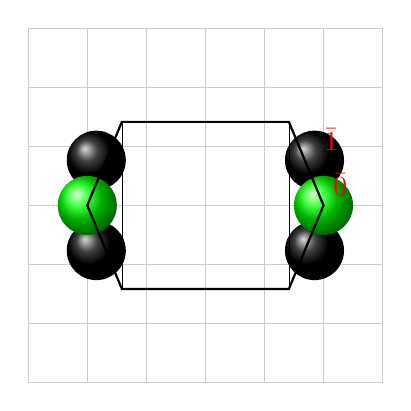
\begin{tikzpicture}[ball color=black,scale=0.75]
		%\draw[ultra nearly opaque] (0,0) circle (2);
		\begin{scope}
		\draw[color=gray!40] (-3,-3) grid (3,3);
		%\shade (45:2) circle (0.5cm) node[anchor=south west,color=red] {$\bar{1}$} ; \shade (135:2) circle (0.5cm)  ; \shade (225:2) circle (0.5cm)  ; \shade (-45:2) circle (0.5cm) ;
		\shade (22.5:2) circle (0.5cm) node[anchor=south west,color=red] {$\bar{1}$} ; \shade (157.5:2) circle (0.5cm)  ; \shade (-157.5:2) circle (0.5cm)  ; \shade (-22.5:2) circle (0.5cm) ;
		\draw[ultra thin] (45:2) -- (135:2) -- (225:2) -- (-45:2) -- cycle;
		\shade[ball color=green] (-2,0) circle (0.5cm)  ; \shade[ball color=green] (2,0) circle (0.5cm)  node[anchor=south west,color=red] {$\bar{0}$} ; 
		\draw[thick] (2,0) -- (45:2) -- (135:2) -- (-2,0) -- (225:2) -- (-45:2) -- cycle;
		\shade[dashed,ball color=red!50,transparent] (0,-2) circle (0.5cm) ;
		\end{scope}
		%\begin{scope}[nearly transparent,dashed,ball color=green,color=red!50]
		%\shade (0,-2) circle (0.5cm) ;
		%\shade (0, 2) circle (0.5cm) ;
		%	\begin{scope}[thin, color=black!50,ultra nearly opaque]
		%	\draw (45:2) -- (0,2) -- (135:2);
		%	\draw (225:2) -- (0,-2) -- (-45:2);
		%	\end{scope}
		%\end{scope}
		\end{tikzpicture}
	\caption{All actual partition rotations plus the quaternion $\boldsymbol{j}$
			do form a group, but together they constitute a valid set of rotations only for partition $\bar{1}$.
		That seems true unless we drop the interpretation of $\boldsymbol{U}$ as list of \textit{normalized column-clusters}. The fundamental relation (\ref{A-N}) 
		doesn't actually require it. With this new freedom, the Hasse space of $\Pi(2)$ seems to map to the (projective) space of vertices of this octagon.}
		\label{octagon}
	\end{figure}
\end{question}
\begin{question}
	What is the geometry of the bipartioning of $3$ elements? From the case of $N=2$ this geometric interpretation of partitions seems to be a subset of $O(2,\mathbb{F}_q)\subset\mathbb{S}^1$. 
	For $N=2$, $q=2$.
\end{question}
\begin{question}
	The octagon is a multiplicative group, and a finite, 2-dim vector space by addition. Can we related to our idea of a "partition-as-a-ket"?
\end{question}
\begin{question}
	We always played  with the posiblity to use a density matrix description. A problem with that was to make sense of a linear combination of \textit{states}.
	Does the octagon represent those states and their linear combinations? The fact that several states represent the same adjacency matrix $\boldsymbol{A}$
	sounds like $\boldsymbol{A}$ is "the observable" to "keep track of"; the \textit{states,} $\boldsymbol{U}$, can change ($\mid\pm\rangle=(1\pm\boldsymbol{j})$). 
	Furthermore, linear combinations or products (as a group) give rise to maps between different Hasse levels.
\end{question}
	\textbf{(Mon Apr 15 2019) Caution!}: If we fix the order of the clusters in $\boldsymbol{\hat{N}}$, \textbf{then there is ONLy 1 such rotation $\boldsymbol{U}$}.

	\textbf{$\bar{0}=1|2$}: The geometric object is isomorphic with $\mathbb{S}^1$, i.e., all rotations in $2$-d fit the bill.

	\textbf{$\bar{1}=12$}: The quaternion corresponding to $\boldsymbol{U}_{12}$ is $\boldsymbol{q}=\frac{1}{2}\{\sqrt{2+\sqrt{2}}\,\mathbbm{1}+\boldsymbol{k}\sqrt{2-\sqrt{2}}\}$.
	Here $\theta/2=22.5^\circ$, where $\boldsymbol{q}=\cos{\theta/2}\mathbbm{1}+\boldsymbol{k}\sin{\theta/2}$.

	The arbitrary choice of rotation axis (i.e., either $\boldsymbol{i},\,\boldsymbol{j},\,\boldsymbol{k}$) doesn't represent any additional degree of freedom.

	Changing $\boldsymbol{k}\to -\boldsymbol{k}$, leads to a different $\boldsymbol{U}$, which entails only a permutation of the cluster columns. Hence, we are also not
	free to change once fixed the order of columns/rows in $\boldsymbol{\hat{N}}$.

	Instead of finding the equivalent quaternion corresponding to rotation $\boldsymbol{U}_{12}$, we could directly interpret this rotation as a quaternion
$\boldsymbol{q}=\frac{1}{\sqrt{2}}\{\mathbbm{1}-\boldsymbol{j}\}$. However, the interpretation as a rotation is that of an angle of $90^\circ$ around
the $\boldsymbol{j}$-axis. uhm...It then seems arbitrary the appearance of the quaternion $\boldsymbol{j}$ instead any of the other two...

	\textbf{In summary: NO OCTAGON!}

	\textbf{$1|23$}: $\boldsymbol{U}=\begin{pmatrix}1&0&0\\0&\frac{1}{\sqrt{2}}&\frac{-1}{\sqrt{2}}\\0&\frac{1}{\sqrt{2}}&\frac{1}{\sqrt{2}}\end{pmatrix}$.
	We have 
	\begin{align*}
		&q_0=\frac{1}{2}\{1+1+\sqrt{2}\}^{1/2}=\frac{1}{2}\sqrt{2+\sqrt{2}}\\
		&q_2=q_3=0\\
		&q_1=\frac{1}{4q_0}(-\epsilon_{123})\boldsymbol{U}_{[2,3]}=\frac{1}{2\sqrt{2+\sqrt{2}}}(\frac{1}{\sqrt{2}}+\frac{1}{\sqrt{2}})=\frac{\sqrt{2-\sqrt{2}}}{2}\\
	\end{align*}
	Hence, $\boldsymbol{q}_{1|23}=\frac{1}{2}\{\sqrt{2+\sqrt{2}}\mathbbm{1}+\boldsymbol{i}\sqrt{2-\sqrt{2}}\}$.

	The reflection, $\boldsymbol{i}\to -\boldsymbol{i}$ leads again to permutation of the cluster columns:
	\begin{eqnarray*}
		q\equiv_{1|23}(\boldsymbol{i}\to -\boldsymbol{i})=\frac{1}{2}\{\sqrt{2+\sqrt{2}}\mathbbm{1}-\boldsymbol{i}\sqrt{2-\sqrt{2}}\}\\
		q^{\dagger}=\frac{1}{2}\{\sqrt{2+\sqrt{2}}\mathbbm{1}+\boldsymbol{i}\sqrt{2-\sqrt{2}}\}\\
		\boldsymbol{qiq^\dagger}=\frac{\boldsymbol{q}}{2}\{\sqrt{2+\sqrt{2}}\boldsymbol{i}-\sqrt{2-\sqrt{2}}\mathbbm{1}\}=\boldsymbol{i}\\
		\boldsymbol{qjq^\dagger}=\frac{\boldsymbol{q}}{2}\{\sqrt{2+\sqrt{2}}\boldsymbol{j}-\sqrt{2-\sqrt{2}}\boldsymbol{k}\}=\frac{1}{2}\{\boldsymbol{j}-\boldsymbol{k}\}\\
		\boldsymbol{qjq^\dagger}=\frac{\boldsymbol{q}}{2}\{\sqrt{2+\sqrt{2}}\boldsymbol{k}+\sqrt{2-\sqrt{2}}\boldsymbol{j}\}=\frac{1}{2}\{\boldsymbol{j}+\boldsymbol{k}\}\\
	\boldsymbol{U}\to \boldsymbol{U}^{'}=\begin{pmatrix}1&0&0\\0&\frac{1}{\sqrt{2}}&\frac{1}{\sqrt{2}}\\0&\frac{-1}{\sqrt{2}}&\frac{1}{\sqrt{2}}\end{pmatrix}
	\end{eqnarray*}

	\textbf{$2|13$}: $\boldsymbol{U}_{2|13}=\begin{pmatrix}0&\frac{1}{\sqrt{2}}&\frac{1}{\sqrt{2}}\\1&0&0\\0&\frac{1}{\sqrt{2}}&\frac{-1}{\sqrt{2}}\end{pmatrix}$.
	We have 
	\begin{align*}
		&q_0=\frac{1}{2}\{1-\frac{1}{\sqrt{2}}\}^{1/2}=\frac{1}{2\sqrt{2}}\sqrt{2-\sqrt{2}}\\
		&q_1=\frac{1}{4q_0}(-\epsilon_{123})\boldsymbol{U}_{[2,3]}=\\
		&q_2=\frac{1}{4q_0}(-\epsilon_{123})\boldsymbol{U}_{[2,3]}=\\
		&q_3=\frac{1}{4q_0}(-\epsilon_{123})\boldsymbol{U}_{[2,3]}=
		\frac{1}{2\sqrt{2+\sqrt{2}}}(\frac{1}{\sqrt{2}}+\frac{1}{\sqrt{2}})=\frac{\sqrt{2-\sqrt{2}}}{2}\\
	\end{align*}
	Hence, $\boldsymbol{q}_{2|13}=\frac{1}{2\sqrt{2}}\{\sqrt{2-\sqrt{2}}\mathbbm{1}+\boldsymbol{i}\sqrt{2+\sqrt{2}}+\boldsymbol{j}\sqrt{2+\sqrt{2}}+\boldsymbol{k}\sqrt{2-\sqrt{2}}\}$.

	This corresponds to $\cos{\theta/2}=\frac{\sqrt{2-\sqrt{2}}}{2\sqrt{2}}\to\;\theta\approx 98.42^\circ$ and 
	$\hat{n}=\frac{1}{\sqrt{6-\sqrt{2}}}\{\sqrt{2+\sqrt{2}}\boldsymbol{i}+...\}$
	and $\widehat{\hat{n} \boldsymbol{i}}\sim 30.36^\circ=\widehat{\hat{n}\boldsymbol{j}}$
	$\widehat{\hat{n} \boldsymbol{k}}\sim 69.06^\circ$
	
%%%%%%%%%%%%%%%%%%%%%%%%%%%%%%%%%%%%%%%%%%%%%%%%%%%%%
%%%%%%%%%% T E N S O R I A L   F O R M 
%%%%%%%%%%%%%%%%%%%%%%%%%%%%%%%%%%%%%%%%%%%%%%%%%%%%%
\subsection{Tensorial form of the fundamental relation}
The previous examples show what seems are general results: while $\mathbf{\hat{N}}$ in Eq.(\ref{A-N}) 
considers $S$ as a set of {\sl indistinguishable elements} ({\sl particles}),
the correct label assignment to each element is provided by the information
contained in the rotation $\mathbf{U}$. 
The sorting of the columns in $\mathbf{U}$ that represent clusters has to be consistent
with that in $\mathbf{\hat{N}}$. Finally, we see that to any given pair of 
equivalence relation $\mathbf{A}$ and size distribution $\mathbf{\hat{N}}$ 
there corresponds two possible family of rotations $\mathbf{U}_{\pm}\in O(N)$ mapping one into the other, 
namely one with determinant $\det({\mathbf{U}_+})=+1$ 
and the other having $\det({\mathbf{U}_-})=-1$. 
These correspond to the remaining degree of freedom in choosing the orientation
of the basis $\{\hat{b}_i\}$ of the null-space of $\mathbf{a}^\dagger$.
As it is only the connected part
of $O(N)$, $SO(N)$, the one which contains the identity, by definition
we will consider rotations $\mathbf{U}\in SO(N)$ only, that is, those with unit determinant.
This representation $\mathbf{U}$ will then be unique modulo any rotation
that preserves the orientation of the null space of $\mathbf{a}^\dagger$. 


Using the tensor product of vectors we can express
definition (\ref{AdjacencyMatrix}) %and (\ref{NumberOperator}) 
directly in terms of the cluster vectors as
\begin{subequations}
\begin{equation}
\mathbf{A}\,=\,\sum_i\,\overrightarrow{a}_i\otimes{\overrightarrow{a}_i}^\dagger
\,=\,\sum_i\,n_i\, \hat{a}_i\otimes \hat{a}_i^\dagger
\end{equation}
where the second equality is exactly Eq.(\ref{A-N}). 
The isometry matrix is given by 
$\mathbf{U}=\begin{bmatrix}
\cdots \hat{a}_i \cdots \hat{b}_j \cdots
\end{bmatrix}
\equiv
\begin{bmatrix}
\cdots \hat{u}_i \cdots 
\end{bmatrix}$.
A more general expression is
\begin{equation}
\mathbf{A}\,=\,\sum_{ij}\,g_{ij}\, \hat{u}_i\otimes \hat{u}_j^\dagger ,
\end{equation}
where it is assumed that $g_{ij}=g_{ji}=0$ if $i>{\cal K}$.
\end{subequations}

For the case of a crisp partition with cluster-size distribution
$\mathbf{\hat{N}}=diag(\{n_i\})$ 
and
writing its general symmetry rotation as
$\mathbf{\Lambda}=[\hat{\Lambda}_1\cdots\hat{\Lambda}_N]$, 
with $\{\hat{\Lambda}_i\}$ an orthonormal set of vectors,
the occupation number matrix is
\begin{equation}
\mathbf{\hat{N}}\,=\,\sum_i\,n_i\,\hat{\Lambda}_i\otimes\hat{\Lambda}_i^\dagger.
\end{equation}



%%%%%%%%%%%%%%%%%%%%%%%%%%%%%%
%%%%%% PARTITIONS ON A GRAPH
%%%%%%%%%%%%%%%%%%%%%%%%%%%%%%
\subsection{Partitions on a graph}
\subsubsection{Cluster decomposition of $\boldsymbol{\omega}$}
Usually, a clustering is defined on a graph $(S,\boldsymbol{\omega})$ of 
weights $\boldsymbol{\omega}_{\alpha\beta}$ between nodes of a set $S$.
We will assume that the graph has no self-loops, i.e.,
that $\boldsymbol{\omega}_{\alpha\alpha}\equiv 0$.
In this section we will introduce some definitions that may become useful later.

The adjacency matrix 
$\boldsymbol{\cal{A}}$ 
of the graph 
%$\boldsymbol{\omega}$, denoted by
is equivalent to $\boldsymbol{\omega}$ by setting
all {\sl relevant} weights to $1$ and the rest to $0$, 
and represents just the topological content of the $\boldsymbol{\omega}$.
Those weights that are relevant will depend on the given graph
and may be defined through a {\sl cut-off} condition as
\begin{subequations}
\begin{equation}
\Xi(\boldsymbol{\omega}_{\alpha\beta}) = 0.
\label{RelevantWeights}
\end{equation}
Then 
$\boldsymbol{\cal{A}}(\boldsymbol{\omega})$ is defined as
\begin{equation}
\boldsymbol{\cal{A}}(\boldsymbol{\omega})_{\alpha\beta}\,\equiv\,
1\,-\,\delta_{0\,\Xi(\boldsymbol{\omega}_{\alpha\beta})}.
\label{AdjacencyMatrixGraph}
\end{equation}
\end{subequations}
For the sake of simplicity, we may think of the simplest case given
by
\begin{subequations}
\begin{eqnarray}
\Xi(\boldsymbol{\omega}_{\alpha\beta}) &=& \boldsymbol{\omega}_{\alpha\beta} \\
\boldsymbol{\cal{A}}(\boldsymbol{\omega})_{\alpha\beta} &=&
1\,-\,\delta_{0\,\boldsymbol{\omega}_{\alpha\beta}}.
\end{eqnarray} 
\end{subequations}

As mentioned above, $\mathbf{a}^\dagger$ provides the
mapping between the space of elements and that of clusters.
Let's work out this projection more in detail.
Given a partition $P$ 
on a graph $\boldsymbol{\omega}$,
we define the {\sl intra-cluster} weights as
\begin{subequations}
\begin{equation}
\boldsymbol{\omega}^<_{\alpha\beta}\,\equiv\,\boldsymbol{\omega}_{\alpha\beta}\,\delta_{P(\alpha)P(\beta)}
\,=\,\boldsymbol{\omega}_{\alpha\beta}\,\overrightarrow{a}_\alpha\cdot\overrightarrow{a}^\dagger_\beta,
\label{IntraClusterWeight}
\end{equation}
where $\overrightarrow{a}_\alpha$ is the $\alpha$-th row vector of matrix $\mathbf{a}$.
Similarly, we define the {\sl inter-cluster} weights as
\begin{equation}
\boldsymbol{\omega}^>_{\alpha\beta}\,\equiv\,\boldsymbol{\omega}_{\alpha\beta}\,
\left[1\,-\,\overrightarrow{a}_\alpha\cdot\overrightarrow{a}^\dagger_\beta\right],
\label{InterClusterWeight}
\end{equation}
such that any weight can be decomposed uniquely as 
$\boldsymbol{\omega}_{\alpha\beta}\,=\,\boldsymbol{\omega}^<_{\alpha\beta}\,+\,\boldsymbol{\omega}^>_{\alpha\beta}$.
\end{subequations}

\begin{subequations}
The sum of all weights within  cluster $i$, $W_i$, is given by
\begin{equation}
W_i\,=\,\frac{1}{2}\overrightarrow{a}_i^\dagger\boldsymbol{\omega}\overrightarrow{a}_i,
\label{ClusterSelfWeight}
\end{equation}
where $\overrightarrow{a}_i$ is the $i$-th column vector of matrix $\mathbf{a}$ 
and the factor $\frac{1}{2}$ corrects the double-counting of edges between any pair 
of elements $\alpha$ and $\beta$. The sum of all intra-cluster weights can
be easily expressed in matrix notation as
\begin{equation}
\sum_i W_i\,=\,\frac{1}{2}Tr\left(\mathbf{a}^\dagger\boldsymbol{\omega}\mathbf{a}\right).
\label{TotalClusterSelfweight}
\end{equation}
In the same way, we can write 
the sum of all weights between clusters $i$ and $j$ as
\begin{equation}
\boldsymbol{W}_{ij}\,\equiv\,\overrightarrow{a}_i^\dagger\boldsymbol{\omega}\overrightarrow{a}_j.
\label{ClusterPairwiseWeight}
\end{equation}
In matrix
notation it is $\boldsymbol{W}\equiv\mathbf{a}^\dagger\boldsymbol{\omega}\mathbf{a}$,
which in tensorial form reads
\begin{equation}
\boldsymbol{W}\,=\,\sum_{\alpha\beta}\,\boldsymbol{\omega}_{\alpha\beta}\,
\overrightarrow{a}_\alpha\otimes\overrightarrow{a}_\beta^\dagger.
\label{ClusterWeightTensorial}
\end{equation}
\end{subequations}

Given a graph $(S,\boldsymbol{\omega})$, the total
weight 
\begin{equation}
\omega\,\equiv\,\sum_{\alpha\beta}\boldsymbol{\omega}_{\alpha\beta}
\,=\,\sum_{\alpha\beta}\left(\boldsymbol{\omega}^<_{\alpha\beta}\,+\,\boldsymbol{\omega}^>_{\alpha\beta}\right)
\label{TotalWeightEdges}
\end{equation}
is invariant under any change of partition $P$ of $S$.
$\omega$ can be decomposed in terms of clusters as
\begin{eqnarray}
\omega\,=\,W &\equiv & \frac{1}{2}\sum_{ij}\boldsymbol{W}_{ij} \nonumber \\
&=& \sum_iW_i\,+\,\sum_{i<j}\boldsymbol{W}_{ij} \nonumber \\
&\equiv & \sum_i \phi_i,
\label{TotalWeightClusters}
\end{eqnarray}
where $\phi_i \equiv W_i + \frac{1}{2}\sum_{i\neq j} \boldsymbol{W}_{ij}$. 

%%%%%%%%%%%%%%%%%%%%%%%%%
%%%%% Spin variables
%%%%%%%%%%%%%%%%%%%%%%%%
\subsubsection{Intrinsic spin variables: Newman's modularity}
In the search for a variational approach to the clustering problem,
a common approach has been to look for an ad-hoc 
order-disorder like hamiltonian 
(See \cite{Blatt96,Shai98,Reichardt06} and references therein). 
This raises the following question:
\begin{question}
Are there some intrinsic {\em spin} variables one may identify in
a graph $(S,\boldsymbol{\omega})$ upon which we can define such
a variational approach?  
\end{question}
The prior information on the problem is in principle very simple, namely that
contained in the graph $\boldsymbol{\omega}$. 
Let's thus try to identify what could be some natural, intrinsic 
spin/momenta variables based solely on that information.

To each node $\alpha$ we can assign a $N$-dimensional vector 
%$\overrightarrow{S}_\alpha\equiv \overrightarrow{\omega}_\alpha$ 
$\overrightarrow{\mu}_\alpha$,
which we call the {\sl topological moment} of node $\alpha$, 
given by all edges spanned by $\alpha$.
, i.e., 
\begin{subequations}
\begin{equation}
\left(\overrightarrow{\mu}_{\alpha}\right)^\gamma \,\equiv\,  \boldsymbol{\cal{A}}(\omega)_{\alpha}^{\gamma}.
\label{MagneticMoment}
\end{equation}
It is straightforward to see that 
$\mu_\alpha^2\equiv\|\overrightarrow{\mu}_\alpha\|^2=\sum_\beta \boldsymbol{\cal{A}}_\alpha^{\phantom{\alpha}\beta}\,
\boldsymbol{\cal{A}}_{\beta\alpha} =k_\alpha $, 
where $k_\alpha$ is the 
degree of node $\alpha$, and 
\begin{equation}
\overrightarrow{\mu}\,\equiv\,\sum_\alpha\,\overrightarrow{\mu}_\alpha\,=\, \overrightarrow{k},
\end{equation}
%with $\overrightarrow{\mu}$ 
is the total topological moment of the graph. 
%We may denote the set of all such spins by $\cal{S}_{\boldsymbol{\omega}}$. 
Then we have 
\begin{equation}
\overrightarrow{\mu}_\alpha\cdot\overrightarrow{\mu}_\beta\,=\,
\text{\# Paths of length 2 from $\alpha$ to $\beta$},
\end{equation}
and in general it is
\begin{equation}
\overrightarrow{\mu}_\alpha^\dagger\,\boldsymbol{\cal A}^l\,\overrightarrow{\mu}_\beta\,=\,
\text{\# Paths of length $2+l$ from $\alpha$ to $\beta$}.
\end{equation}
A {\em self-loop}  of an element $\alpha$ 
can be assigned a 
moment $\overrightarrow{\mu}_\alpha^o$ 
which coincides 
with the base vector representing the element itself $e_\alpha$.
Thus, even if the graph $\boldsymbol{\omega}$ has no self-loops,
we can view $e_\alpha$ as the moment of a {\em virtual} self-loop
$\protect\overrightarrow{\mu}^0_\alpha$
that
is related to the moment of $\alpha$ as 
$\boldsymbol{\cal A}(\boldsymbol{\omega})\protect\overrightarrow{\mu}^0_\alpha=
\boldsymbol{\cal A}(\boldsymbol{\omega})e_\alpha=
\protect\overrightarrow{\mu}_\alpha$. 
This allows us to express the number of paths of length $l$ 
between elements $\alpha$ and $\beta$ in the usual form
namely as powers of the adjacency matrix of the given graph,
\begin{equation}
%\overrightarrow{\mu}_\alpha\cdot\overrightarrow{\mu}_\beta\,=\,
\overrightarrow{\mu}_\alpha^0\boldsymbol{\cal A}^l(\boldsymbol{\omega})\overrightarrow{\mu}_\beta^0.
\end{equation}
For $l=1$ and $\alpha=\beta$ this gives the number of actual self-loops
for each node $\alpha$, which we assume to be zero, i.e., 
$\protect\overrightarrow{\mu}_\alpha^0
\boldsymbol{\cal A}(\boldsymbol{\omega})
\protect\overrightarrow{\mu}_\alpha^0=0$. 
\end{subequations}

%Draw a node; 1 args is center point
\newcommand{\vertex}[1]{\put(#1){\circle*{.025}}}
%Draw an edge as thinline; 3 args same as \line
\newcommand{\edge}[3]{{\thinlines \put(#1){\line(#2){#3}}}}
%Draw an aggregate Edge (sum of edges) as thickline; 3 args same as \line
\newcommand{\Edge}[3]{{\thicklines \put(#1){\line(#2){#3}}}}
%Draw a labeled cluster as a circle; 2 args, center and label
\newcommand{\cluster}[2]{\thicklines \put(#1){$#2$}\put(#1){\circle{0.2}}}
\begin{figure}
\setlength{\unitlength}{0.5\columnwidth}
%\setlength{\unitlength}{5cm}
\begin{picture}(1,1)(0,0)
\put(0,.8){$A)$}
\thicklines
\cluster{.5,.7}{i}
\put(0.1,.45){$\alpha$}
\vertex{0.2,.5}
%\put(0.3,.5){\line(3,2){0.25}}
%\Edge{0.3,.5}{3,2}{.25}
%% \thinlines
%% \qbezier(0.3,.5)(.4,.9)(0.56,0.67)
%% \thicklines
\put(.2,.65){$S^i_\alpha$}
\Edge{.2,.5}{1,1}{.22}
\Edge{.2,.5}{3,2}{.26}
\put(.85,.45){$\beta$}
\vertex{.8,.5}
\put(.8,.65){$S^i_\beta$}
\Edge{.8,.5}{-1,1}{.22}
\Edge{.8,.5}{-3,2}{.26}
%\dottedline{0.005}(.5,.75)(.6,.45)
\end{picture}
\begin{picture}(1,1)(0,0)
\put(0,.8){$B)$}
\thicklines
\put(.5,.9){\line(0,-1){.5}}
\put(.05,.5){$\alpha$}
\vertex{.06,.6}
\put(.2,.8){$S^i_\alpha$}
\Edge{.06,.6}{2,1}{.44}
\Edge{.06,.6}{3,1}{.44}
\put(.95,.5){$\beta$}
\vertex{.96,.6}
\put(.7,.8){$S^i_\beta$}
\Edge{.96,.6}{-2,1}{.45}
\Edge{.96,.6}{-3,1}{.45}
\put(.35,.2){$\overrightarrow{S}_\alpha\cdot\overrightarrow{S}_\beta \geq 0$}
%% \thinlines
%% \qbezier(.05,.54)(.45,.8)(.5,.7)
%% \qbezier(.95,.54)(.55,.8)(.5,.7)
\end{picture}
\caption{Graphical representation of the intrinsic spin variables in the graph clustering problem. 
$A)$ $S^i_\alpha$ ($S^i_\beta$) is total number of edges between node $\alpha$ ($\beta$) and cluster $i$. 
$B)$ The scalar product of two spins
%$\overrightarrow{S}_\alpha \cdot \overrightarrow{S}_\beta$ 
yields the sum of all 2-edges paths joining nodes $\alpha$ and $\beta$. The vertical line
denotes the summation over all clusters.
}
\label{SpinVariables}
\end{figure}

\begin{subequations}
Furthermore, ${\mathbf{a}}^\dagger$ maps $\overrightarrow{\mu}_\alpha$ to
a $\cal{K}$-dimensional vector $\overrightarrow{S}_\alpha$, 
which we call the {\sl spin} of node $\alpha$,
where each component $i$
is the number of edges starting on $\alpha$ and ending in cluster $i$, as
given by
\begin{equation}
\overrightarrow{S}_\alpha \,\equiv\, {\mathbf{a}}^\dagger \overrightarrow{\mu}_\alpha
\,=\,\left[\overrightarrow{a}_i\cdot\overrightarrow{\mu}_\alpha\right]
\label{Spin}
\end{equation}
Thus, the mapping $\overrightarrow{a}^\dagger$ represents a
change of representation from one based on nodes to one based on clusters.
It is straightforward to see that 
$\overrightarrow{\Sigma}_{\alpha}\equiv \mathbf{a}\overrightarrow{S}_\alpha$ represents
the same information in the space of all nodes, i.e., each component $\beta$,
\begin{equation}
\left(\overrightarrow{\Sigma}_{\alpha}\right)^{\beta}\,=\,\left(\mathbf{a}\overrightarrow{S}_\alpha\right)^\beta\,=\,
\delta^{P(\beta)}_{P(\gamma)}\,\boldsymbol{\cal{A}}(\omega)_{\alpha}^{\gamma},
\end{equation}
is the number of edges starting at node $\alpha$ and ending at the cluster containing
node $\beta$. 
%% The following symbolic relation holds
%% \begin{equation}
%% \overrightarrow{S}_\alpha\,:=\,\overrightarrow{a}^\dagger \mathbf{A}(P)^{-1} \overrightarrow{\Sigma}_\alpha,
%% \end{equation}
%% as $\mathbf{A}(P)$ is only invertible for $P=\bar{0}$.
\end{subequations}

Newman and Girvan's modularity measure is given by\cite{Newman04}
\begin{subequations}
\begin{equation}
Q \equiv \sum_i \left[\frac{e_i}{M}\,-\,\left(\frac{\sum_{\alpha\in C_i}k_\alpha}{2M}\right)^2\right], 
\label{Modularity}
\end{equation}
where $e_i$ is the number of intra-cluster edges for cluster $C_i$ 
and $M=\sum_{\alpha\leq\beta}\boldsymbol{\cal A}_{\alpha\beta}$ is the total number of edges in the graph.
Hence, the
different terms in (\ref{Modularity}) can be rewritten as
\begin{eqnarray}
\sum_{\alpha\in C_i}\,k^\alpha &=& \overrightarrow{a}_i\cdot\overrightarrow{k} \,=\, \sum_\alpha\,S^i_\alpha \\
\sum_i\,\left(\sum_{\alpha\in C_i}\,k^\alpha\right)^2 &=&
\sum_i\,\left(\overrightarrow{a}_i\cdot\overrightarrow{k}\right)^2\,=\,
\sum_{\alpha\,\beta}\,\overrightarrow{S}_\alpha\cdot\overrightarrow{S}_\beta \,=\,
\nonumber\\
 &=&   
 \left(\mathbf{a}^\dagger\,\overrightarrow{\mu}\right)\cdot\left(\mathbf{a}^\dagger\,\overrightarrow{\mu}\right)
 \,\equiv\,\overrightarrow{S}\cdot\overrightarrow{S},
\end{eqnarray}
\end{subequations}
where $\overrightarrow{S}$ is the total spin of the graph,
and the modularity is
\begin{equation}
Q\,=-{\cal H}({S})\,\equiv\,\frac{1}{2M}\sum_{\alpha}\,\overrightarrow{S}_\alpha\cdot\overrightarrow{a}_\alpha\,-\,\frac{1}{4M^2}
\sum_{\alpha\,\beta}\,\overrightarrow{S}_\alpha\cdot\overrightarrow{S}_\beta
\label{ModularitySpin}
\end{equation}
which has a structure akin to that of a spin-system Hamiltonian with long-range interactions
in the presence of an external field ${\overrightarrow{a}_\alpha}$.
A similar conclusion was already stated in \cite{Reichardt06} although they started
from an ad-hoc Potts Hamiltonian that already conveyed the form of the modularity.
It is straightforward to see that the second term in Eq.(\ref{ModularitySpin}) is always
negative, vanishing only for the trivial case of a network ${\cal A}(\boldsymbol{\omega})$
with no edges. Technically, the optimal partition would then remain undertermined.
We will then convey to choose partition $\bar{0}$ as the optimal partition. 
For any two elements $\alpha$ and $\beta$, this term
is more negative the more edges these elements have that end in the same cluster.
It, therefore, tends to split the system into as many clusters as possible. 
Conversely, the first term attains its maximum value when each node has edges only
within the same cluster it belongs to, i.e., it favors partition $\bar{1}$, the clustering
of all elements together. 
This spin model thus shares some similiraties with that of an antiferromagnet, 
but as opposed to usual treatments of the latter model, 
the spin-spin interactions in Eq.(\ref{ModularitySpin})
contain all pairs of spins. One is tempted to consider it then as a model 
with long-range interactions. This, however, seems somewhat misleading, as it
is not clear what the meaning of distance on the network is, nor what the
dimensionality of the system is. 
%% For example, the case of $N=4$ spins could
%% be viewed as a system of nearest-neighbor interactions embeded in a 
%% $2$-dimensional space with the topology of the M\"obius strip. 

\begin{figure}
%\begin{center}
\subfloat[P=$23|1$]{\label{A}\includegraphics[width=0.5\textwidth]{Figures/SpinRotations/Spinrotations23-1.jpg}}
\\
\subfloat[P=$12|3$]{\label{B}\includegraphics[width=0.5\textwidth]{Figures/SpinRotations/Spinrotations12-3.jpg}}
%% \subfloat{\label{A}\includegraphics[width=0.5\textwidth]{Spinrotations23-1.jpg}}
%% \subfloat{\label{B}\includegraphics[width=0.5\textwidth]{Spinrotations12-3.jpg}}
\caption{%
Spin rotations. The effect of two different partition rotations on the topological
momenta (continuous arrows) of $3$ elements is shown for two partitions defined
on the same network $2-1-3$: (\ref{A}) $P=23|1$
and (\ref{B}) $P=12|3$. The rotated 
momentum $\mathbf{U}^\dagger\protect\overrightarrow{\mu}_\alpha$ is shown in dotted lines.
Dash-dotted arrows indicate the spin $\protect\overrightarrow{\sigma}_\alpha$ (filled arrowheads)
and the hole spin (hollow arrowhead) $\protect\overrightarrow{\tau}_\alpha$, such that 
$\protect\overrightarrow{\mu}^{'}_\alpha=
\mathbf{U}^\dagger\mu_\alpha=\protect\overrightarrow{\sigma}_\alpha+\protect\overrightarrow{\tau}_\alpha$,
where we define $\protect\overrightarrow{\sigma}_\alpha\equiv\mathfrak{\hat{a}}^\dagger\,\mu_\alpha$ 
and $\protect\overrightarrow{\tau}_\alpha\equiv\mathfrak{\hat{b}}^\dagger\,\mu_\alpha$.
Because of symmetry, the spins of elements $2$ and $3$ coincide.
}
%\end{center}
\label{DispersionHoleSpin}
\end{figure}

As $S^i_\alpha$ depends itself on $\mathbf{a}$,
the product  
%the previous interpretation of 
$\overrightarrow{S}_\alpha\cdot\overrightarrow{a}_\alpha$ 
%as an {\em external} field 
does not correspond exactly to what
is usually considered as the action of an
external field on a local spin variable.
However, we may uncouple spin and external
field by writing the modularity in terms of
the topological momenta.

Let us consider the action of a partition rotation $\mathbf{U}$ 
on the topological momentum $\overrightarrow{\mu}_\alpha$ of an
element $\alpha$.
\begin{eqnarray}
\mathbf{U}^\dagger\,\overrightarrow{\mu}_\alpha &=& 
\mathfrak{\hat{a}}^\dagger\,\overrightarrow{\mu}_\alpha
\,+\,
\mathfrak{\hat{b}}^\dagger\,\overrightarrow{\mu}_\alpha \nonumber\\
&\equiv & \overrightarrow{\sigma}_\alpha\,+\,\overrightarrow{\tau}_\alpha,
\end{eqnarray}
which defines the 
{\em dispersion spin} $\overrightarrow{\sigma}_\alpha = \mathfrak{\hat{a}}^\dagger\overrightarrow{\mu}_\alpha$ 
and {\em hole spin} $\overrightarrow{\tau}_\alpha  = \mathfrak{\hat{b}}^\dagger\overrightarrow{\mu}_\alpha$.
See figure (\ref{DispersionHoleSpin}). It is straightforward to see that
\begin{equation}
\overrightarrow{\sigma}_\alpha^\dagger\cdot\overrightarrow{\sigma}_\beta\,=\,
\sum_i\,\overrightarrow{\mu}_\alpha^\dagger\,
%\frac{\overrightarrow{a}_i\,\otimes\,\overrightarrow{a}_i^\dagger}{n_i}\,
\hat{a}_i\,\otimes\,\hat{a}_i^\dagger\,
\overrightarrow{\mu}_\beta
=\sum_i\,\frac{S^i_\alpha\, S^i_\beta}{n_i},
\end{equation}
where its module is bound by $|\sigma_\alpha^i | \lesssim \sqrt{n_i}$ 
and $\|\overrightarrow{\sigma}_\alpha\|\lesssim\,{\cal K}\sqrt{n_i}$.
We have then
\begin{equation}
\overrightarrow{\sigma}_\alpha^\dagger\,\mathbf{\hat{N}}\,\overrightarrow{\sigma}_\beta\,=\,
\overrightarrow{\mu}_\alpha^\dagger\,\mathbf{A}\,\overrightarrow{\mu}_\beta\,=\,
\sum_i\,S^i_\alpha\,S^i_\beta.
\end{equation}
The following projection yields the action of 
$\protect\overrightarrow{a}_\alpha$ on the spin of element $\beta$
\begin{equation}
\overrightarrow{\sigma}_\alpha^{o\dagger}\,\mathbf{\hat{N}}\,\overrightarrow{\sigma}_\beta\,=\,
%\overrightarrow{\mu}_\alpha^{o\dagger}\,\mathbf{A}\,\overrightarrow{\mu}_\beta\,=\,
\overrightarrow{\mu}^0_\alpha\,\mathbf{A}\,\overrightarrow{\mu}_\beta\,=\,
\sum_i\,\left(\overrightarrow{a}_\alpha\right)^i\,S^i_\beta.
\end{equation}
%% We will call 
%% \begin{equation}
%% \overrightarrow{h}_\alpha\,\equiv\,\mathbf{A}\,e_\alpha
%% \end{equation}
%% the {\em external field} defined by the partition $\mathbf{A}$. 
Then we can write the modularity as
\begin{equation}
%Q\,=-{\cal H}(\{\overrightarrow{\mu}_\alpha\})\,\equiv\,\frac{1}{2M}
Q\,=-{\cal H}\,\equiv\,\frac{1}{2M}
\sum_{\alpha}\,\overrightarrow{\mu}_\alpha\cdot\overrightarrow{a}_{P(\alpha)}
\,-\,\frac{1}{4M^2}
\sum_{\alpha\,\beta}\,\overrightarrow{\mu}_\alpha\,\mathbf{A}\,\overrightarrow{\mu}_\beta,
\label{ModularityTopMomenta}
\end{equation}
where now the external field $\protect\overrightarrow{a}_{P(\alpha)}$ is 
homogenous over the elements belonging to the same cluster.
This can be written in a more compact form as
\begin{equation}
Q\,=\,-{\cal H}\,=\,r\,\sum_\alpha\,
%\langle\overrightarrow{\mu}_\alpha | \overrightarrow{\mu}^o_\alpha\rangle_{\mathbf{A}}\,-\,
\overrightarrow{\mu}_\alpha *_{\mathbf{A}} \overrightarrow{\mu}^o_\alpha\,-\,
r^2\,\sum_{\alpha\beta}\,
%\langle\overrightarrow{\mu}_\alpha | \overrightarrow{\mu}_\beta\rangle_{\mathbf{A}},
\overrightarrow{\mu}_\alpha *_{\mathbf{A}} \overrightarrow{\mu}_\beta,
\end{equation}
with $r=\frac{1}{2M}$ and 
$\overrightarrow{v}*_{\mathbf{A}}\protect\overrightarrow{w}\equiv
\langle\protect\overrightarrow{v}|\protect\overrightarrow{w}\rangle_{\mathbf{A}}
=\mathbf{A}_{\alpha\beta}v^\alpha w^\beta$,
where $\mathbf{A}(P)$ plays the role of a pseudo-metric 
in the vectorial space of momenta of the 
nodes of graph $\boldsymbol{\omega}$ (see Eq.(\ref{GramMatrix})).

Let us consider two partition $\mathbf{A}^n$ and $\mathbf{A}^m$ corresponding to
the same cluster-size distribution $\mathbf{\hat{N}}$. As we have
seen above, there is a relative rotation $\mathbf{R}_{mn}$ such that 
$\mathbf{A}^m=\mathbf{R}_{mn}\mathbf{A}^n\mathbf{R}_{mn}^\dagger$.
Therefore, the modularity $Q^m$ corresponding to partition $\mathbf{A}^m$
can be seen as the modularity of a partition $\mathbf{A}^n$ with
a network whose momenta are rotated by 
$\mathbf{R}_{mn}^\dagger\protect\overrightarrow{\mu}_\alpha$ 
relative to the original network.
%This leads us to consider 
This suggests the possibility of 
an alternative way of looking at the partitioning problem
of a complex network:
instead of searching for the optimal partition given a fixed
topology, we can view it as searching for the optimal topology
for a fixed partition, albeit the network now becomes a weighted
network. For such a view to hold, it would be necessary to find
a positive answer to the following question:
\begin{question}
Given two partitions
corresponding to two different cluster-size distributions,
can we find a rotation that transforms 
them into each other?
\end{question}
As shown in question $\boldsymbol{Q}$\ref{QTransfAcrossHasseLevels}, this has a partially positive answer.
Indeed, the similarity transformation between partitions with different cluster-size distributions
is given by an isometry of $\boldsymbol{l_1}$ and not $\boldsymbol{l_2}$.

%The present result (\ref{ModularitySpin}), 
The present result (\ref{ModularityTopMomenta}) 
has been obtained without
any ad-hoc assumptions of the number of spin states nor other parameters, contrary
to the departing Ansatz of \cite{Reichardt06}, and it simply
shows that the modularity of Newman and Girvan is in essence but 
an order-disorder like Hamiltonian. 
Moreover, (\ref{ModularitySpin}) identifies what is a
genuine definition of the spin of a node $\overrightarrow{S}_\alpha$ 
relevant to the clustering problem, namely 
as a projection onto the cluster space of 
a column of the adjacency matrix of the graph $\boldsymbol{\omega}$. 
We will be able to substantiate such a claim
only if we can show that the Hamiltonian ${\cal H}({S})$ can effectively be used
to derive a sound clustering algorithm, much like it was done in \cite{Reichardt06}.

In the quest for finding a sound (spin) Hamiltonian analog for the clustering problem,
Reichardt and Bornholdt...

%%%%%%%%%%%%%%%%%%%%%%%%%%
%
\section{Symmetry of communities in complex networks\label{secLieAlgebra}}
We will demonstrate in this section how the concept of ideal (boolean) partition
bears in essence the recognition of a symmetry in the distribution of weights
over the set of clusters given by $\boldsymbol{W}$.

\subsection{The partition Lie algebra $\mathfrak{p}(N,{\cal K})$}
%We have seen before that 
As per Eq.(\ref{ClusterWeightTensorial}), 
this distribution has a tensorial representation
given by $\boldsymbol{W}=\sum_{\alpha\beta}\boldsymbol{\omega}_{\alpha\beta}\eta_{\alpha\beta}$ with
\begin{equation}
\eta_{\alpha\beta}\,\equiv\,\overrightarrow{a}_\alpha\otimes\overrightarrow{a}_\beta^\dagger.
\label{generators-PLieAlgebra}
\end{equation}
We will show now that the operators $\eta_{\alpha\beta}$ define a Lie algebra
describing the symmetries of the distribution of weights $\boldsymbol{W}$ among
clusters $\mathbf{a}$, which we will call the partition Lie algebra. 
To each Hasse level, i.e., to each number of clusters ${\cal K}$ 
corresponds different representations of this algebra. We will therefore
denote this algebra in general by $\mathfrak{p}(N,{\cal K})$. 

Bilinear products of fermion or boson creation and annihilation operators
allow for the introduction of Lie algebras that have been proven to be
extremely useful in quatum field theory and many-particle systems \cite{Lipkin65}. 
For instance, the isospin can be obtained by considering all
bilinear products of neutron and proton creation and annihilation 
operators which do not change the number of particles. We will show
that the generators (\ref{generators-PLieAlgebra}) can also be 
interpreted in a similar way. 

Clearly, the set of operators in Eq.(\ref{generators-PLieAlgebra}) is redundant.
For all elements 
$\alpha'\,,\beta'$ such that $P(\alpha')=P(\alpha)\,,P(\beta')=P(\beta)$ it is
$\eta_{\alpha'\beta'}=\eta_{\alpha\beta}$, as the definition Eq.(\ref{generators-PLieAlgebra})
depends only on the clusters elements $\alpha$ and $\beta$ belong to.
Therefore, it is convenient to change to a notation dependent only on the clusters
labels given by
\begin{subequations}
\begin{align}
\boldsymbol{W} &= \sum_{ij}\,\boldsymbol{W}_{ij}\,\eta_{ij} \\
\boldsymbol{W}_{ij} &= 
 \sum_{\alpha\beta}\,\boldsymbol{\omega}_{\alpha\beta}\delta_{iP(\alpha)}\,\delta_{jP(\beta)} \\
\eta_{ij} &\equiv \delta_{iP(\alpha)}\delta_{jP(\beta)}
 \overrightarrow{a}_\alpha\otimes\overrightarrow{a}_\beta^\dagger.
\end{align}
\label{CanonicalGeneratorsPLieAlgebra}
\end{subequations}

The generators of the partition Lie algebra satisfy the commutation rules
\begin{subequations}
\begin{equation}
\left[\eta_{\alpha\beta},\eta_{\alpha'\beta'}\right]\,=\,
\lambda_{\alpha\beta\alpha'\beta'}^{\mu\nu}
\eta_{\mu\nu}
\end{equation}
with structure factors given by
\begin{equation}
\lambda_{\alpha\beta\alpha'\beta'}^{\mu\nu}\,\equiv\,
\delta^\mu_\alpha\,\delta^\nu_{\beta'}\,\delta_{P(\beta)P(\alpha')}
\,-\,
\delta^\mu_{\alpha'}\,\delta^\nu_{\beta}\,\delta_{P(\alpha)P(\beta')}.
\end{equation}
It is straightforward to prove that the matrices $\eta_{\alpha\beta}$
satisfy the Jacobi identity
\begin{widetext}
\begin{equation}
0\,=\,
\left[\eta_{\alpha\beta}\,,\,\left[\eta_{\alpha'\beta'}\,,\,\eta_{\alpha''\beta''}\right]\right]
\,+\,
\left[\eta_{\alpha'\beta'}\,,\,\left[\eta_{\alpha''\beta''}\,,\,\eta_{\alpha\beta}\right]\right]
\,+\,
\left[\eta_{\alpha''\beta''}\,,\,\left[\eta_{\alpha\beta}\,,\,\eta_{\alpha'\beta'}\right]\right].
\end{equation}
\end{widetext}
\end{subequations}
The following properties hold
\begin{subequations}\label{etaProperties}
\begin{align}
\eta_{\alpha\beta}\,\eta_{\alpha'\beta'}\,=\,\delta_{P(\beta)P(\alpha')}\,\eta_{\alpha\beta'} \\
\eta_{\alpha\beta}^2\,=\,\delta_{P(\alpha)P(\beta)}\,\eta_{\alpha\beta} \\
Tr(\eta_{\alpha\beta})\,=\,\delta_{P(\alpha)P(\beta)} \\
\boldsymbol{\hat{N}}\,=\,\sum_\alpha\,\eta_{\alpha\alpha} \label{PAlgebraNumberConstraint}\\
\left[\boldsymbol{\hat{N}}\,,\,\eta_{\alpha\beta}\right]\,=\,(n_\alpha\,-\,n_\beta)\,\eta_{\alpha\beta}\\
\left[\boldsymbol{\hat{N}}\,,\,\eta_{\alpha\beta}^2\right]\,=\,0,
\end{align}
with $n_\alpha$ a short-hand notation for the number of elements
in the cluster containing $\alpha$, i.e., $n_\alpha\equiv n_{P(\alpha)}$. 
\end{subequations}
We have as well for the structure factors 
\begin{subequations}\label{strucFactProperties}
\begin{align}
\lambda_{\alpha\beta\alpha'\beta'}^{\mu\nu}\,\in\,\{-1\,,\,0\,,\,1\} \\
\lambda_{\alpha\beta\alpha'\beta'}^{\mu\nu} \,=\, -\lambda_{\alpha'\beta'\alpha\beta}^{\mu\nu} \\
\lambda_{\alpha\beta\alpha'\beta'}^{\mu\nu}\,\delta_{P(\mu)P(\nu)}\,=\,0 \\
\lambda_{\alpha\alpha\beta\beta}^{\mu\nu}\,=\,
\left(
\delta^\mu_\alpha\delta^\nu_\beta\,-\,\delta^\mu_\beta\delta^\nu_\alpha
\right)\,\delta_{P(\alpha)P(\beta)}.
\end{align}
The dimension of the matrices $\eta_{\alpha\beta}$ is ${\cal K}\times{\cal K}$ and 
there are ${\cal K}^2-1$ independent generators, due to condition Eq.(\ref{PAlgebraNumberConstraint}),
giving rise to the lie algebra 
%$\mathfrak{su}({\cal K}({\cal K}-1)/2)$.
$\mathfrak{p}({\cal N},{\cal K})\subset \mathfrak{su}({\cal K})$.
\end{subequations}

The introduction of the partition algrebra $\mathfrak{p}({\cal N},{\cal K})$
is a trivial consequence of working on a linear space. The matrix $\mathbf{W}$
belongs in fact to a ${\cal K}\times{\cal K}$-dimensional linear space, which
has a {\sl canonical base} given by the ${\cal K}\times{\cal K}$ matrices 
${e}_{ij}\equiv \delta_{ij}$. We are free, however, to choose any other
set of ${\cal K}\times{\cal K}$ independent matrices as a base for such a linear
space. The generators $\eta_{\alpha\beta}$ simply represent such an
example, as do any other combination of them. The following specific
examples will help clarifying these points. This trivial nature of 
the Lie algebra $\mathfrak{p} ({\cal N},{\cal K})$ means, in particular, that it can
be defined in any {\sl vectorial} space with a non-conmutative 
internal product\cite{Hestenes84}. 

The actual relevance of the partition algebra lies in the fact that it 
allows us to define the ideal partition in terms of a symmetry requirement
on the distribution of weights among the different clusters. 
It is invariance under rotations in the {\sl cluster} space
that characterizes the intuitive and widespread idea of 
{\sl ideal partition}, as we will
see later. This concept of symmetry in the clustering problem 
explains the recurrent approach found hitherto in the literature
of using the concept of spin, e.g., in the form of a Pott-model, when
looking for suitable mathematical descriptions. Each {\sl spin value} is there 
tantamount to a cluster label. We will show below
that the full concept of spin as an invariant observable under
certain transformations can carried over to the partitioning
problem.

%%%%%%%%%%%%%%%%%%%%%%%%%%%%%%%%%%%%%%%55
%%%%%%%%%%%%%
\subsection{Isospin of the graph-bisectioning problem}
Let's consider the lie algebra associated to the
case $N=2$ and ${\bar 0}_2=1|2$. We have the following 
generators:
\begin{subequations}
\begin{align}
\eta_{12}=
\begin{pmatrix}
1 \\ 0
\end{pmatrix} \otimes
\begin{pmatrix}
0 & 1
\end{pmatrix}
=
\begin{pmatrix}
0 & 1 \\
0 & 0
\end{pmatrix}
\\
\eta_{21}=
\begin{pmatrix}
0 \\ 1
\end{pmatrix} \otimes
\begin{pmatrix}
1 & 0
\end{pmatrix}
=
\begin{pmatrix}
0 & 0 \\
1 & 0
\end{pmatrix}
\\
\eta_{11}=
\begin{pmatrix}
1 & 0 \\
0 & 0 
\end{pmatrix}
\quad\quad
\eta_{22}=
\begin{pmatrix}
0 &0 \\
0 &1
\end{pmatrix}
\end{align}
\end{subequations}
with the number operator given by $\boldsymbol{\hat{N}}=\eta_{11}+\eta_{22}$.
We introduce now the {\em isospin} operators
\begin{subequations}
\begin{align}
\boldsymbol{\tau}_+&\equiv\eta_{12}  &\boldsymbol{\tau}_-\equiv\eta_{21} \\
\boldsymbol{\tau}_0&\equiv\frac{1}{2}\left(\eta_{11}-\eta_{22}\right).
\end{align}
The properties (\ref{etaProperties}) imply that 
they all commute with $\boldsymbol{\hat{N}}$ 
and we also have the commutation rules
\begin{align}
\begin{split}
\left[\boldsymbol{\tau}_0,\boldsymbol{\tau}_+\right] &=
\frac{1}{2}\left[\eta_{11},\eta_{12}\right]
-
\frac{1}{2}\left[\eta_{22},\eta_{12}\right]
\\&=\frac{1}{2}(\eta_{12}+\eta_{12})\\ &=\boldsymbol{\tau}_+
\end{split}
\\
\left[\boldsymbol{\tau}_0,\boldsymbol{\tau}_-\right] &=-\boldsymbol{\tau}_- \\
\left[\boldsymbol{\tau}_+,\boldsymbol{\tau}_-\right] &=2\boldsymbol{\tau}_0.
\end{align}
\label{SchwingerOscillatorModelAngularMomentum}
\end{subequations}
In quantum mechanics this corresponds to the isospin algebra where 
$\boldsymbol{\hat{N}}$ is the barion number operator and the charge 
operator $\boldsymbol{Q}$ is defined through the relation 
$\boldsymbol{\tau}_0=\boldsymbol{Q}-\frac{1}{2}\boldsymbol{\hat{N}}$,
which in our case is $\boldsymbol{Q}=\eta_{11}$. 
In the present case, obviously, the {\em charge of a cluster} is
just an arbitrary label for denoting each cluster.

%Following a common trend in text books of quantum mechanics,
We define the {\em complex} operators of {\em angular momentum}
\begin{subequations}
\begin{align}
\boldsymbol{J}_x &\equiv\frac{1}{2}\left(\boldsymbol{\tau}_++\boldsymbol{\tau}_-\right)
=\frac{1}{2}\left({\eta}_{12}+{\eta}_{21}\right)\\
\boldsymbol{J}_y &\equiv\frac{1}{2i}\left(\boldsymbol{\tau}_+-\boldsymbol{\tau}_-\right)
=\frac{-i}{2}\left({\eta}_{12}-{\eta}_{21}\right)\\
\boldsymbol{J}_z &\equiv\boldsymbol{\tau}_0.
\end{align}
It is easy to see that these operators do satisfy the
well-known commutation rules of angular momentum
\begin{align}
\left[\boldsymbol{J}_x,\boldsymbol{J}_y\right]=i\boldsymbol{J}_z \\
\left[\boldsymbol{J}_z,\boldsymbol{J}_x\right]=i\boldsymbol{J}_y \\
\left[\boldsymbol{J}_y,\boldsymbol{J}_z\right]=i\boldsymbol{J}_x,
\end{align}
and that they commute with the casimir operator 
$\boldsymbol{J}^2\equiv\boldsymbol{J}_x^2+\boldsymbol{J}_y^2+\boldsymbol{J}_z^2$.
The latter in addition is related to the (barion) number operator as
\begin{equation}
\boldsymbol{J}^2=\frac{3}{4}\boldsymbol{\hat{N}}=\frac{1}{2}(\frac{1}{2}+1)\boldsymbol{\hat{N}}.
\label{Spin1/2}
\end{equation} 
\label{AngularMomentum1/2}
\end{subequations}
We see therefore that the partition Lie algebra
conveys the expected symmetry which hitherto in the literature 
had been assigned in an ad-hoc fashion. 
Indeed, relation (\ref{Spin1/2}) corresponds precisely  to that
of a system with angular momentum  $j=1/2$, 
as one would define for any partition with only two clusters.
In the Physics literature, Eqs.(\ref{SchwingerOscillatorModelAngularMomentum})
are known as Schwinger's Oscillator model of Angular Momentum.

Talking about partition ${\bar 0}_2$ as having a spin, or angular momentum
of $1/2$ is again a short-hand notation for describing
the fact that it consists of only two clusters. If this
would be the only benefit, introducing these concepts into the
clustering problem would certainly be
an overkill.
The powerful tools of Lie algebras, however, will
unveil further consequences of that fact when partioning
a complex graph $\boldsymbol{\omega}$. This in turn
should provide for a proper justification of their use.

A technical remark is in place here. In rigor, we have not demonstrated
that the Lie algebra
derived here is that of $\mathfrak{su}(2)$. For that we would need to show 
that, indeed, the algebra relevant to clustering would be the
Lie algebra over the real numbers spanned by $\{i\,\boldsymbol{J}_i\}$.
Therefore, so far, we will consider that the Lie algebra 
unfolded by the bipartitioning problem is 
(a subalgebra of) $\mathfrak{sl}(2,\mathbb{C})$.

%%%%%%%%%%%%%%%%%%%%%%%%%%%%
% 
\subsection{$\mathfrak{su}(3)$ symmetry}
Let's consider the partition ${\bar 0}_3=1|2|3$. 
The partition Lie algebra contains $9$ independent
operators given by
\begin{subequations}
\begin{align}
\boldsymbol{\hat{N}}&=\eta_{11}+\eta_{22}+\eta_{33}\\
\boldsymbol{\tau}_+ &=\eta_{12}\quad\quad\boldsymbol{\tau}_-=\eta_{21} \\
\boldsymbol{\tau}_0 &=\frac{1}{2}\left(\eta_{11}-\eta_{22}\right)\\
\boldsymbol{B}_+    &=\eta_{13}\quad\quad\boldsymbol{B}_-=\eta_{23} \\
\boldsymbol{C}_+    &=\eta_{32}\quad\quad\boldsymbol{C}_-=\eta_{31} \\
\boldsymbol{M}      &=\frac{1}{3}\left(\eta_{11}+\eta_{22}-2\eta_{33}\right) .
\end{align}
\end{subequations}
These satisfy the commutation rules of the Lie algebra $\mathfrak{su}(3)$,
as we will discuss next.
First we note that
\begin{subequations}
\begin{align}
\begin{split}
\left[\boldsymbol{\tau}_0,\boldsymbol{B}_{\pm}\right] 
&=\frac{1}{2}\{\left[\eta_{11},\eta_{\pm 3}\right]-\left[\eta_{22},\eta_{\pm 3}\right]\} \\
&=\frac{1}{2}\eta_{\pm 3} \\
&=\pm \frac{1}{2}\boldsymbol{B}_{\pm}
\end{split}
\\
\left[\boldsymbol{\tau}_0,\boldsymbol{C}_{\pm}\right] &=\pm\frac{1}{2}\boldsymbol{C}_{\pm},
\end{align}
where $\eta_{\pm3}$ is a short-hand notation for $\eta_{13}$ and $\eta_{23}$.
\end{subequations}
Therefore, $\boldsymbol{B}_+$ and $\boldsymbol{C}_+$ 
{\em create a (cluster-)$1$ particle and annihilate a (cluster-)2 particle}
respectively. These commutation relations are thus consistent with
interpreting the tensorial product (\ref{generators-PLieAlgebra})
$\eta_{\alpha\beta}\equiv\protect\overrightarrow{a}_\alpha\otimes\protect\overrightarrow{a}_\beta^\dagger$
as equivalent to the bilinear form 
$\boldsymbol{a}^\dagger_\alpha\boldsymbol{a}_\beta$ 
of creation and annihilation operators in Quantum Field Theory.
That is, $\eta_{\alpha\beta}$ creates an {\em $\alpha$ particle/excitation}
and {\em destroys a $\beta$ particle}.

We further have thus that the operators $\boldsymbol{B}_{\pm}$
annihilate a (cluster-)$3$ particle and therefore increase 
$\boldsymbol{M}$ by $+1$, while the operators $\boldsymbol{C}_{\pm}$
create a (cluster-)$3$ particle, and thus change 
$\boldsymbol{M}$ by $-1$. A simmilar argument leads
to the fact that the opertors $\boldsymbol{\tau}_{0,\pm}$,
however, leave $\boldsymbol{M}$ unchanged. This yields the additional
commutation rules
\begin{subequations}
\begin{align}
\left[\boldsymbol{M},\boldsymbol{B}_{\pm}\right] &= \boldsymbol{B}_{\pm} \\
\left[\boldsymbol{M},\boldsymbol{C}_{\pm}\right] &= -\boldsymbol{C}_{\pm} \\
\left[\boldsymbol{M},\boldsymbol{\tau}_{0,\pm}\right] &= 0.
\end{align}
The remaining commutation rules are
\begin{align}
\begin{split}
\left[\boldsymbol{\tau}_{\pm},\boldsymbol{B}_{\pm}\right]
&=\left[\boldsymbol{\tau}_{\pm},\boldsymbol{C}_{\pm}\right]\\
&=\left[\boldsymbol{B}_{+},\boldsymbol{B}_{-}\right]\\
&=\left[\boldsymbol{C}_{+},\boldsymbol{C}_{-}\right]=0  
\end{split}
\\
\left[\boldsymbol{\tau}_{\pm},\boldsymbol{B}_{\mp}\right] &= \boldsymbol{B}_{\pm} \\
\left[\boldsymbol{\tau}_{\pm},\boldsymbol{C}_{\pm}\right] &= -\boldsymbol{C}_{\mp} \\
\left[\boldsymbol{B}_{\pm},\boldsymbol{C}_{\mp}\right] 
&=\frac{1}{2}\left(3\boldsymbol{M}\pm 2\boldsymbol{\tau}_0\right) \\
\left[\boldsymbol{\tau}_{0},\boldsymbol{\tau}_{\pm}\right] &=\pm\boldsymbol{\tau}_{\pm} \\
\left[\boldsymbol{\tau}_{+},\boldsymbol{\tau}_{-}\right] &= \boldsymbol{\tau}_0.  
\end{align}
The previous relations define the well-known Lie algebra of $\mathfrak{su}(3)$.
\end{subequations}

\subsection{Symmetries of the Weight Distribution}
Defining a partition on a weighted network $\boldsymbol{\omega}$
entails a particular distribution of these weights among all
clusters (communities) given by $\boldsymbol{W}$. 
It is common in the literature to guide the search for an
optimal partition through the following criterion: 
If $\boldsymbol{\omega}$ represents a measure of similarity,
the optimal partition is such that the inter-cluster similarity
 vanishes (or, eventually, is as low as possible) while the
 intra-cluster similarity is as high as possible.
We shall now show that this criterion can be expressed as a 
condition of symmetry on $\boldsymbol{W}$.

Let's first consider the case of a bipartitioning, ${\cal K}=2$.
From the previous discussion in this section, we see that 
$\boldsymbol{W}$ can be expressed as a function of the generators
of $\mathfrak{sl}(2,\mathbb{C})$, say 
$\boldsymbol{W}=\boldsymbol{W}(\boldsymbol{J}_i)$.
The symmetry properties of $\boldsymbol{W}$ are 
given by the following commutators:
\begin{subequations}
\begin{align}
\left[\boldsymbol{W}\,,\,\boldsymbol{J}_i\right] &= 
 \sum_{\alpha\,\beta}\,\omega_{\alpha\,\beta}\,\left[\eta_{\alpha\,\beta}\,\,\boldsymbol{J}_i\right] \\
\left[\boldsymbol{W}\,,\,\boldsymbol{J}^2\right] &= 
 \sum_{\alpha\,\beta}\,\omega_{\alpha\,\beta}\,\left[\eta_{\alpha\,\beta}\,\,\boldsymbol{J}^2\right]
\end{align}
As the generators $\eta_{\alpha\beta}$ depend only the cluster, we can collect terms and simplify it to
\begin{align}
\left[\boldsymbol{W},\boldsymbol{J}_i\right] &= 
	\boldsymbol{W_{11}}\left[\eta_{11},\boldsymbol{J}_i\right] +\boldsymbol{W_{22}}\left[\eta_{22},\boldsymbol{J}_i\right]+2\boldsymbol{W_{12}}\left[\boldsymbol{J}_x,\boldsymbol{J}_i\right]\\
\left[\boldsymbol{W},\boldsymbol{J}^2\right] &= 
	\boldsymbol{W_{11}}\left[\eta_{11},\boldsymbol{J}^2\right] +\boldsymbol{W_{22}}\left[\eta_{22},\boldsymbol{J}^2\right]+2\boldsymbol{W_{12}}\left[\boldsymbol{J}_x,\boldsymbol{J}^2\right]
\end{align}
Plugging in Eqs.(\ref{AngularMomentum1/2}), it is straightforward to see that 
\begin{align}
\left[\boldsymbol{W}\,,\boldsymbol{J}^2\right] &= 0 \\
\left[\boldsymbol{W}\,,\boldsymbol{J}_x\right] &= 
 \phantom{-}i\,\left(\boldsymbol{W}_{11}\,-\,\boldsymbol{W}_{22}\right)\,\boldsymbol{J}_y\\
\left[\boldsymbol{W}\,,\boldsymbol{J}_y\right] &= 
 -i\,\left(\boldsymbol{W}_{11}\,-\,\boldsymbol{W}_{22}\right)\,\boldsymbol{J}_x
 \,+\,\boldsymbol{J}_z\,\boldsymbol{W}_{12} \\
\left[\boldsymbol{W}\,,\boldsymbol{J}_z\right] &= 
 -i\,\boldsymbol{J}_y\,\boldsymbol{W}_{12} \label{JzConservation-bisec}
\end{align}
\end{subequations}

Therefore, a fully $\mathfrak{sl}(2,\mathbb{C})$ symmetric weight distribution
requires that I) the total sum of intercluster weights be zero and 
II) all intra-cluster partial sums be equal. We also see that the common
requirement for an optimal partition of vanishing intercluster weight entails
the rotational symmetry around axis $z$. 
The additional conserved quantity (besides the total number of elements) is
the $z$-component of spin (label: up/down) assigned to each cluster.

In other words, Eq.(\ref{JzConservation-bisec}) puts on formal grounds the connection
between the intuitive criterion of vanishingly small inter-cluster weight
and the possibility of discerning between two different clusters.
 
For the case of partitions with three clusters we can proceed in an analogous way.
$\mathfrak{su}(3)$ has $8$ generators ${G_i}$. We are interested in the commutators of them and the weight distribution tensor:
\begin{eqnarray}
%\begin{align}
	\left[\boldsymbol{W}\,,\boldsymbol{G}_i\right] &=& 
	\boldsymbol{W_{11}}\left[\eta_{11},\boldsymbol{G}_i\right] +\boldsymbol{W_{22}}\left[\eta_{22},\boldsymbol{G}_i\right]+
	\boldsymbol{W_{33}}\left[\eta_{33},\boldsymbol{G}_i\right]\nonumber\\
	&+&\sum_{l<m=1}^3\boldsymbol{W_{lm}}\left[\left(\boldsymbol{\eta}_{lm}+\boldsymbol{\eta}_{ml}\right),\boldsymbol{G}_i\right]
%\end{align}
\end{eqnarray}

%%%%%%%%%%%%%%%%%%%%%%%%%%
\section{Statistical Mechanics\label{secStatMech}}
\subsection{On a microcanonical description}
Consider the problem of clustering a set of $N$ homeodomain protein sequences.
%Thus, even 
As discussed in section \ref{BayesianApproach}, 
even if we are given just with $N$ elements to cluster, we can always consider
such a system as a sample of a much larger set $N'$.
For the combined set, we can then write the affinity matrix as
\begin{equation}
\boldsymbol{w}\,=\,
\left(
\begin{array}{ccccccc|c}
 & & & & & & & \\
 & & & & & & & \\
 & & & & & & & \\
 & & & \boldsymbol{w}_B & & & & \boldsymbol{w}_{BS} \\
 & & & & & & & \\
 & & & & & & & \\
 & & & & & & & \\\hline
 & & & & & & & \boldsymbol{w}_S 
\end{array}
\right)\nonumber
\end{equation}
and the total weight can be split as sum of the total weight of
our system $S$, that of the additional larger set $B$ and that of
their correlation (interaction) as  
\begin{equation}
\omega\,=\,\omega_S\,+\,\omega_B\,+\,\omega_{BS}.
\end{equation}
When considering only the set (system) $S$ of $N$ sequences,
$B$ is akin to the {\sl rest of the universe} (of homeodomains)
within which the former has been isolated. That is, there has been
a process of identifying $S$ as distinct from the rest (clustering),
and a step of {\sl erasure} of (that) information 
and its substitution by an uncertainty $\Delta$ in both $\omega_B$ and $\omega_S$.
The rationale is as follows: Differences in the curation step while gathering the initial data $T=B+S$,
as well as differences in the clustering step, will mean that, if we
have two observers independently doing this work, both will end up with
a different set of sequences (nodes), and hence affinities 
(i.e., edges contributing to $\omega_B$ and $\omega_S$) as well,
for both subsystems $B$ and $S$. If the initial data allows for a clear distinction of both
subsets
and the accuracy of both procedures is similar, we expect the difference $\Delta$ 
in total weight $\omega$ to be  small. 
%(INTERESTING! WORTH DEVELOPING FURTHER?).  
In the case when
\begin{equation}\label{WeaklyInteractingSystems}
|\omega_{BS}|\,\ll\,|\omega_S| ,\,|\omega_B|
\end{equation}
both subsets $B$ and $S$ are weakly correlated 
and we will also denote such a case as that of two weakly {\sl interacting} systems.
If in addition we have $N_B\gg N$ and
\begin{equation}\label{HeatBathCondition}
|\omega_{BS}|\,\ll\,|\omega_S|\,\ll\,|\omega_B|,
\end{equation} 
we may consider the system $B$
as akin to the concept of {\sl heat bath} in statistical mechanics.

Let us consider a fixed topology of the network $\Xi(\omega_{\alpha\beta})$.
In general, the number of affinity configurations ({\sl states}) $\boldsymbol{\omega}$ 
of the system $T=B+S$ compatible
with $\omega$ is a function of $\omega$ and $N'=N_B+N$, $\Omega_T(\omega,N')$.
However, this is no longer true when $B$ is acting as a heat bath for $S$
as, by definition, in such a case the condition (\ref{HeatBathCondition})
must hold. In particular, this condition will rule out all those distribution of affinity values
for which $|\omega_{BS}|\lesssim|\omega_S|$ \{MAKES SENSE?\}.


The following description closely follows the arguments in \cite{FeynmanStatMech}.
What are the number of {\sl states} $\Omega$ compatible with a given value of $\omega$?
%% For a fixed graph $\boldsymbol{\omega}$, $\Omega$ is given by the number of
%% partitions of $N$ elements $\Gamma_N\equiv\|\Pi (N)\|$. Furthermore, for a given partition $P\in\Pi (N)$,
The set of states compatible with $\omega$ forms a continuous $d_{\boldsymbol{\omega}}\equiv N(N-1)/2-1$ 
dimensional hyperplane according to 
(\ref{TotalWeightEdges}) and (\ref{TotalWeightClusters})
\begin{equation}
0\,=\,\sum_{\alpha<\beta}\,d\omega_{\alpha\beta}.
\label{OmegaMicrocanonical}
\end{equation}
The number of states with a total weight at most $\omega$, for large $\omega$, 
is proportional to $\omega^{d_{\boldsymbol{\omega}}}$, so that the number of states per unit 
weight range is 
$\eta (\omega) \propto (d/d\omega)\omega^{d_{\boldsymbol{\omega}}} \propto \omega^{d_{\boldsymbol{\omega}} -1}$.
We would like to identify 
\begin{equation}
\beta\equiv \frac{d\log\eta(\omega )}{d\omega}\,=\,\frac{d_{\boldsymbol{\omega}} -1}{\omega}
\end{equation}
with the parameter that controls the probability of having the system with
total weight $\omega$
\begin{equation}
\mathcal{P}(\omega)\,\propto\,e^{-\beta \omega},
\label{TotalWeightStatMech}
\end{equation}
the dependence on $\Gamma_N$ being  included in the proportionality constant.
Implicitly, it is assumed that there is no absolute scale for the weights 
$\boldsymbol{\omega}_{ij}$, but only weight differences matter.

Clearly, %due to (\ref{TotalWeightClusters}), 
a description like (\ref{TotalWeightStatMech}) does not allow us to 
infer the most likely clustering
out of the information contained in $\boldsymbol{\omega}$, as it is
$\Omega\,=\,\Omega (\omega, N)$. Rather, what we
are looking for is a description $\mathcal{P}(\boldsymbol{\omega},\boldsymbol{a})$ that
contains both the information on the graph as well as on the partition. Such a 
description could convey the intuitive idea that not all partitions fit equally well a given
affinity graph $\boldsymbol{\omega}$.

We define the {\sl ideal partition} $\boldsymbol{a}^E$ (or {\sl equilibrium} partition) 
as one for which
the inter-cluster weights are negligible in comparison to the intra-cluster weights, i.e.,
\begin{equation}
W\,=\,\frac{1}{2}\sum_i \boldsymbol{W}_{ii} \,+\, \sum_{i<j} \boldsymbol{W}_{ij}\,\simeq\,
\frac{1}{2}\sum_i \boldsymbol{W}_{ii}\,+\,\cdots
\label{IdealPartition}
\end{equation}
Here {\sl ideal} is meant as 
an idealized simple solution much like in {\sl ideal gas} in physics,
and {\sl equilibrium} is meant as the {\sl true} solution. 


For such a description, the details of the partition $\boldsymbol{a}$
will become essential. From the definition, the system is composed of ${\cal K}\equiv\|P\|$
independent and {\sl non-interacting} clusters. Thus
\begin{equation}
W^E\,\simeq\,\sum_i W_i\,=\,\frac{1}{2}Tr(\boldsymbol{a}^{E\dagger}\boldsymbol{\omega}\boldsymbol{a}^E).
\label{TotalEnergyIdealPartition}
\end{equation}
Swapping elements between clusters, in general, will change the total weight $W^E$ by way
of adding a term of inter-cluster interaction
\begin{equation}
W^E\,\rightarrow\,\sum_i W^\prime_i\,+\,\sum_{kl}\boldsymbol{W}^{\prime}_{kl}.
\end{equation}
Now, the set of {\sl microstates} compatible with a given $W^E$ is 
no longer the whole space $\Pi_N$. 
Most importantly, now it is $\Omega\,=\,\Omega (\boldsymbol{\omega},\boldsymbol{a}^E)$,
where the dependency on $N$ is already included in $\boldsymbol{\omega}$ and $\boldsymbol{a}^E$.


%%%%%%%%%%%%%%%%%%%%%%%%%%%%
%%%%%%%%     APPENDICES
%%%%%%%%%%%%%%%%%%%%%%%%%%%%
\begin{appendix}
%%%%%%%%%%%%%%%%%%%%%%%%%%%%%%%%%%%%
%%%%%%%% Non information-theoretic distances
%%%%%%%%%%%%%%%%%%%%%%%%%%%%%%%%%%%
\section{Non-information theoretic distances}
Other distances can also be defined, e.g., the van Dongen distance used in MCL, which
we will not discuss in this work. Another interesting distance is the Tarantola distance \cite{Tarantola},
for which we need to introduce the corresponding Jeffrey function for a partition
$J(P)$. This should be a unique, non-negative defined function for each partition.
The Tarantola distance between two partitions $P$ and $Q$ is then defined as
\begin{equation}
d_s(P,Q)\,\equiv\,\left|\log\,\frac{J(P)}{J(Q)}\right|
\end{equation}
Alternatively, we may introduce a distance based on the rotation matrix $\boldsymbol{U}(P)$ associated
to a partition $P$ (Eq. \ref{A-N}).
\begin{equation}
d_m(P,Q)\,\equiv\,\left\|\log\,\frac{\boldsymbol{U}(P)}{\boldsymbol{U}(Q)}\right\|,
\label{TarantolaDistanceMatrix}
\end{equation}
where the norm of a matrix is defined as 
$\|\boldsymbol{U}\|^2=\frac{1}{2}\,Tr\,\boldsymbol{U}^\dagger\boldsymbol{U}$.
This is a sound definition of distance as $\boldsymbol{U}$ is a symmetric, positive-definite matrix.

It is important to remark that 
such a distance cannot be defined using the adjacency matrix $\boldsymbol{A}(P)$ of
$P$, as in general it is not invertible -that is true, for instance, 
whenever there are no singletons.
The same applies for any
undirected graph $\boldsymbol{\omega}$  
as, in general, it is a singular matrix.
%it is only semi-positive definite matrices.
However, we can consider the traceless part of $\boldsymbol{A}(p)$
given by $\boldsymbol{A}_0\equiv\boldsymbol{A}-\boldsymbol{1}_{N\times N}$.
Analogously, we can introduce a {\sl topological distance} by
applying definition (\ref{TarantolaDistanceMatrix}) to the 
adjacency matrix ${\cal A}_\omega$.
%% allows
%% to introduce the equivalent {\sl topological distance} 
%% between two graphs $\boldsymbol{\omega}$ and $\boldsymbol{\omega}'$ as 
%% $d_m(\boldsymbol{{\cal A}}_{\boldsymbol{\omega}},\boldsymbol{{\cal A}}_{\boldsymbol{\omega}'})$.
%% Let's define $E_0$ as the smallest integer closest to the smallest eigenvalue of $\boldsymbol{\omega}$.
%% Then $\boldsymbol{\Omega}\equiv\boldsymbol{\omega}-E_0$ is also symmetric and positive definite
%% and we define the distance between two (weighted) graphs as
%% \begin{equation}
%% d_m(\boldsymbol{\Omega},\boldsymbol{\Omega}')
%% \,\equiv\,
%% \left\|\log\,\frac{\boldsymbol{\Omega}}{\boldsymbol{\Omega}'}\right\|
%% \end{equation}

Provided with such distance $d_m(P,Q)$, the space of (fuzzy) partitions acquires a 
structure that is not necessarily that of a flat (Euclidean) space\cite{Tarantola}. A geodesic, relative
to the metric $d_m(P,Q)$, can then be defined joining any pair of partitions $P$ and $Q$.
An interesting question then arises: 
\begin{question}
is there \emph{always} a geodesic between $P$ and $Q$
that  includes partition $P\wedge Q$? If that would be the case, we could write without
loss of generality $d_m(P,Q)=d_m(P,P\wedge Q)+d_m(P\wedge Q, Q)$.
\end{question} 
as well as
\begin{question}
Can we define a non-information theoretic distance for which its associate
geodesics always include $P\wedge Q$?
\end{question} 

Being a rotation, we can always write $\boldsymbol{U}$  in exponential form
as $U(P)=e^{i\,\overrightarrow{\theta_P}\cdot \overrightarrow{\boldsymbol{J}}}$,
where $\theta^i_P\in\mathbb{R}$ and $\boldsymbol{J}^i$ are skew-symmetric matrices
that form the associated Lie algebra $\mathfrak{su}(N)$.
Taking the logarithm we can write it as 
$\log \boldsymbol{U}\,=\,i\,\overrightarrow{\theta_P}\cdot \overrightarrow{\boldsymbol{J}}$,
where the logarithm will be given by
\begin{subequations}
\begin{equation}
\log\,\boldsymbol{U}\,=\,\boldsymbol{C}\,\log\,\hat{\boldsymbol{U}}\,\boldsymbol{C}^\dagger
\end{equation}
where $\hat{\boldsymbol{U}}$ is the diagonal matrix of the eigenvalues of $\boldsymbol{U}$
and $\boldsymbol{C} \in SU(N)$ is a unitary matrix. Thus, in this representation
we will deal with complex matrices $\hat{\boldsymbol{U}}$ and $\boldsymbol{C}$ 
despite $\boldsymbol{U}$ being real valued.

Let's consider the examples of section \ref{ExamplesRotations},
$P_2=1|23$ and $P_2''=12|3$.
For $P_2$, $\boldsymbol{U}_2$ has eigenvalues 
$\{1,\lambda_{\pm}=\frac{(1\pm i)}{\sqrt{2}}=e^{\pm i\,\theta_2}\}$, with 
$\theta_2=\pi/4$, and we have
\begin{eqnarray}
\hat{\boldsymbol{U}}_{2} &=& diag(1,e^{i\,\frac{\pi}{4}},e^{-i\,\frac{\pi}{4}}) \\
\boldsymbol{C}_2           &=& 
\begin{bmatrix}
1 & 0                  & 0 \\
0 & \frac{\lambda_+}{\sqrt{2}} & \frac{-\lambda_+}{\sqrt{2}} \\
0 & \frac{\lambda_-}{\sqrt{2}} & \frac{\lambda_-}{\sqrt{2}}
\end{bmatrix},
\end{eqnarray}
which yields
\begin{equation}
\log\,\boldsymbol{U}_2\,=\,
\begin{bmatrix}
0 & 0 & 0 \\
0 & 0 & -\theta_2 \\
0 & \theta_2 & 0 
\end{bmatrix} 
\,=\,-i\,\theta_2\,
\begin{bmatrix}
0 & 0 & 0 \\
0 & 0 & -i \\
0 & i & 0 
\end{bmatrix} 
\,=\,-i\,\theta_2\,\boldsymbol{\lambda_7}
\end{equation}
where $\boldsymbol{\lambda_7}$ is one of the
corresponding Gell-Mann matrices that form the Lie algebra of $\mathfrak{su}(3)$.
Therefore it is
\begin{equation}
\|\log \boldsymbol{U}_2\|\,=\,\theta_2\,=\,\frac{\pi}{4}.
\end{equation}
\end{subequations}

Analogously for $P_2''$, $\boldsymbol{U}_2''$ has eigenvalues
$\{1,\lambda_\pm =\frac{-(2-\sqrt{2})\pm i\,\sqrt{10+4\sqrt{2}}}{4}=e^{\pm\,i(\pi-\theta_{2}'')}\}$,
where $\theta_2''=\arctan (\frac{\sqrt{10+4\sqrt{2}}}{2-\sqrt{2}})$ and 
\begin{subequations}
\begin{equation}
\boldsymbol{C}_2''\,=\,
\begin{bmatrix}
  \frac{1}{n_1}             & \frac{\lambda_+}{n_2}            & \frac{\lambda_-}{n_2} \\
  \frac{1+\sqrt{2}}{n_1}    & \frac{1+\sqrt{2}\lambda_+}{n_2}  & \frac{1+\sqrt{2}\lambda_-}{n_2} \\
  \frac{1}{n_1}             & \frac{1}{n_2}                     & \frac{1}{n_2}        
\end{bmatrix},
\end{equation}
where $n_1=\sqrt{5+2\sqrt{2}}$ and $n_2=\sqrt{3-\frac{1}{\sqrt{2}}}$, 
such that
\begin{equation}
\log \boldsymbol{U}_2''\,=\,\eta\,(\pi-\theta_2'')\,
\begin{bmatrix}
%% 0 & 7\sqrt{2}-8 & -(6-\sqrt{2}) \\
%% -(7\sqrt{2}-8) & 0 & 7\sqrt{2}-8 \\
%%  6-\sqrt{2}& -(7\sqrt{2}-8) & 0
0 & a & -b \\
-a & 0 & a\\
b & -a & 0
\end{bmatrix},
\end{equation}
with $a=7\sqrt{2}-8$, $b=6-\sqrt{2}$ and $\eta=\frac{\sqrt{10+4\sqrt{2}}}{2(19-6\sqrt{2})}$.
Its norm is
\begin{eqnarray}
\|\log \boldsymbol{U}_2''\| &=& \pi\,-\,\theta_2''\,=\, \\
&=& \pi\,-\,
\arctan\left(
\frac{\sqrt{10-4\sqrt{2}}}{2-\sqrt{2}}
\right)\,\sim\,0.5468\,\pi. \nonumber
\end{eqnarray}
\end{subequations}


As it is $P_2\wedge P_2''=\bar{0}$ 
and the rotation associated to partition $\bar{0}$ is the identity, we have
\begin{eqnarray}
d_m(P_2,\bar{0}) &=& \|\log \boldsymbol{U}_2\|\,=\,\frac{\pi}{4} \\
d_m(P_2'',\bar{0}) &=& \|\log \boldsymbol{U}_2''\|\,\sim\, 0.5468\,\pi\,\ge\,\frac{5\pi}{12}.
\end{eqnarray}
We want to compare these distances with that between $P_2$ and $P_2''$
\begin{equation}
d_m(P_2,P_2'')=\|\log \frac{\boldsymbol{U}_2}{\boldsymbol{U}_2''}\|=
%\|\log \boldsymbol{U}_2\,{\boldsymbol{U}_2''}^\dagger\|=
\|\log
\begin{bmatrix}
0 & 0 & 1 \\
1 & 0 & 0 \\
0 & 1 & 0
\end{bmatrix}
\|\,=\,\frac{2\,\pi}{3}.
\end{equation}

%%%%%%%%%%%%%%%%%%%%%%%%%%%%%%%%%%%%%%%%%%%
%% METRIC GENERATING FUNCTION
%%%%%%%%%%%%%%%%%%%%%%%%%%%%%%%%%%%%%%%%%%
\section{Metric-generating function}
\newcommand{\figsSA}{
\begin{figure}
\setlength{\unitlength}{\columnwidth}
\begin{picture}(1,0.8)
\thicklines
\put(0.49,.77){$\bar{1}$}
\put(0.5,.75){\circle*{.025}}

\thinlines
\put(0.5,.75){\line(1,-1){0.3}}
\put(0.8,.45){\circle*{.025}}
\put(0.82,0.435){$R\wedge Q$}

\put(0.5,.75){\line(-1,-1){0.3}}
\put(0.2,.45){\circle*{.025}}
\put(0.08,.435){$P\wedge R$}

\thicklines
\put(0.5,.15){\line(1,1){0.3}}
\put(0.5,.15){\line(-1,1){0.3}}
\put(0.5,.15){\circle*{.025}}
\put(0.412,0.1){$P\wedge Q\wedge R$}

\thinlines
\dashline{0.025}(.5,.75)(.4,.35)
%\put(0.5,.75){\line(-1,-4){0.1}}
\put(0.4,.35){\circle*{.025}}
\put(0.42,0.335){$P\wedge Q$}

\dashline{0.025}(.5,.75)(.6,.50)
%\put(0.5,.75){\line(1,-3){0.1}}
\put(0.6,.50){\circle*{.025}}
\put(0.62,.495){$R$}

\thicklines
\dashline{0.05}(.4,.35)(.5,.15)
\dashline{0.05}(.6,.50)(.5,.15)
%\put(0.4,.35){\line(1,-2){0.1}}
%\put(0.6,.45){\line(-1,-3){0.1}}

\put(0.2,0.05){$D_{F}\equiv 2g(P\wedge Q\wedge R)-g(P\wedge R)-g(R\wedge Q)$}
\put(0.2,0.0){$D_{I}\equiv 2g(P\wedge Q\wedge R)-g(P\wedge Q)-g(R)$}
\end{picture}
\caption{Hasse Diagram describing condition $s$SA (\ref{SSA2}).
Two partitions are joined by a line if (the lower) one is a perfect refinement
of the other. 
The distance between $P\wedge R$ and $R\wedge Q$,
$D_{F}$, is shown as a continuous bold line, 
and that between $P\wedge Q$ and $R$,
$D_{I}$, as a long-dashed bold line.
The question is:
is it always $D_{I}\,\ge\,D_{F}$ ? The functions $g$ for which that is
true are said to satisfy the special-strong subadditivity condition and give
rise to the algorithmic complexity (or VI) distance metric in $\Pi$. 
}
\label{Fig:sSa}
\end{figure}
}

%%%%%%%%%%%%%%%%%%%
\subsection{Special-strong subadditivity}
We define a scalar field $g(P)$ in $\Pi$ as a function that maps any partition to a real number. 
For any given scalar field $g$ and all $P, Q, R \in \Pi$, define 
$\Delta_g\left(P,Q;R\right) \equiv g(P\wedge R)+g(R\wedge Q)-g(P\wedge Q)-g(R)$. 
We introduce the following 
\begin{definition}
We will say that the scalar field $g$ on $\Pi$
satisfies the special-strong subadditivity ($s$SA)condition if 
for all $P, Q, R \in \Pi$ it holds that
\begin{equation}
%&(\text{G:\quad $\forall P,Q,Z \in\Pi$})&\nonumber\\
\Delta_g\left(P,Q;R\right) \geq 0.
%&g(P\wedge Q)\,+\,g(R)\leq\,g(P\wedge R)\,+\,g(R\wedge Q)&
%(\text{G2})&g(P\wedge Q)\,\leq\,g(P)\,+\,g(Q)&(\text{Subadditivity})
\label{SSA2}
\end{equation}
\end{definition}
Below We will justify refering to (\ref{SSA2}) as a subadditivity condition.
In this section, we will discuss some important consequences
of property (\ref{SSA2}). 

%In particular, %we have that % $s$SA implies
\begin{lema}
If a scalar function $g$ on $\Pi$ satisfies the special-strong subadditivity
condition ($s$SA), then it holds
\begin{equation}
%(\text{G1}) \, 
P \triangleleft R \,\Rightarrow\,g(P)\,>\,g(R). \label{Monotonicity}
%(\text{G2}) & g(P)\,=\,0\,\Leftrightarrow\, P={\bar 1} & \label{ZeroEntropy}.
\end{equation}
\end{lema}
Property (\ref{Monotonicity}), which we may call monotonicity, expresses 
the compatibility of  $g$ with the lattice structure of $\Pi$. This follows
trivially from (\ref{SSA2}) by taking $Q=\bar{0}$ % \,\text{or}\, \bar{1}$ 
and using (\ref{OrderIntersection}).

Hence, as $\Pi$ is a compact lattice, it follows the following 
\begin{corolary}
If $g$ satisfies $s$SA, then it has a minimum and a maximum on $\Pi$ given by 
$g(\bar{1})$ and $g(\bar{0})$ respectively. 
\end{corolary}
%%$\inf_{P\in\Pi}g(P)\,=\,g(\bar{1})$ and $\sup_{P\in\Pi}g(P)\,=\,g(\bar{0})$ respectively. 
%% Without loss of generality, we
%% will assume that $g(\bar{1})\equiv 0$. Thus, condition (\ref{ZeroEntropy}) states
%% that $\ker (g)=\{\bar{1}\}$. This property follows immediately from (\ref{Monotonicity})
%% by considering any $P\neq\bar{1}$ and $Q=\bar{1}$.
%% Note that properties $G1$ and $G2$ imply that $g\geq 0$, i.e, 
%% the metric-generating function is positive defined. This is not strictly necessary for
%% $G1$ guaranties that $\Delta\Delta g\geq 0$. 

We are particularly interested in defining and charectizing a distance metric
in the space $\Pi$ of all partitions.
\begin{definition}
We will say that $g(P)$ is a {\sl metric-generating} function on $\Pi$ (MGF) when for any 
$P,\,Q\,\in\Pi$ 
%We will show that 
the function $d(P,Q)$ defined as 
\begin{equation}
d(P,Q)\,\equiv\,\left|\Delta\,g_{P,Q}\right|\,\equiv\,\left|g(P)\,-\,g(Q)\right|
\label{PseudoMetric}
\end{equation}
is a pseudometric in $\Pi$ and the function
$D(P,Q)$ defined as
\begin{equation}
D(P,Q)\equiv\left| g(P\wedge Q) - g(P)\right| + \left|g(P\wedge Q) - g(Q)\right|,
\label{Metric}
\end{equation}
which, using the monotonicity property (\ref{Monotonicity}) , can be written as
\begin{equation}
D(P,Q)=\Delta\Delta\,g_{P,Q}\,\equiv\, 2\,g\left(  P\,\wedge\,Q\right)\,-\,g(P)\,-\,g(Q ),
\label{ThermoMetric}
\end{equation}
is a metric in the space of all partitions. 
\end{definition}
In that way, each metric-generating function
$g(p)$ defines a unique distance in $\Pi$. 
An interesting question is to find the most general conditions for a scalar 
field $g$ to be a MGF on $\Pi$. Here we will address a more modest goal of 
stating a sufficient condition:

\begin{lema}
\label{T-SSA2}
%% For all $P, Q, R \in \Pi$, define 
%% $\Delta_g\left(P,Q;R\right) \equiv g(P\wedge R)+g(R\wedge Q)-g(P\wedge Q)-g(R)$. 
The family of scalar fields $g$ on $\Pi$ satisfying the
special-strong subadditivity condition (\ref{SSA2}) 
%%property
%% \begin{equation}
%% %&(\text{G:\quad $\forall P,Q,Z \in\Pi$})&\nonumber\\
%% \Delta_g\left(P,Q;R\right) \geq 0
%% %&g(P\wedge Q)\,+\,g(R)\leq\,g(P\wedge R)\,+\,g(R\wedge Q)&
%% %(\text{G2})&g(P\wedge Q)\,\leq\,g(P)\,+\,g(Q)&(\text{Subadditivity})
%% \label{SSA2}
%% \end{equation}
is a set of MGFs. 
\end{lema}
\begin{proof}
Let us prove Lema \ref{T-SSA2}. We need to show that 
$D(P,Q)$ is indeed a distance in $\Pi$. Clearly, it is a symmetric
function of $P$ and $Q$, i.e., $D(P,Q)=D(Q,P)$ and it is positive defined. 
Also, from (\ref{Monotonicity}) %(\ref{ConditionalEntropy}) 
we have $D(P,Q)=0\Leftrightarrow P=Q$.
Thus, we only need to demonstrate that $D(P,Q)$ also satisfies the triangular inequality
\begin{equation}
\forall P,Q,R \in \Pi \; ;\; D(P,Q)\,\leq\,D(P,R)\,+\,D(R,Q).\nonumber
\label{TriangleInequality}
\end{equation}
Inserting \ref{ThermoMetric} into the r.h.s. of this relation, %\ref{TriangleInequality}
we obtain
\begin{equation}
D(P,R)\,+\,D(R,Q)\,=\,2\,f(P,Q,R)\,+\,D(P,Q)\nonumber
\end{equation}
with $f(P,Q,R)$ such that
\begin{equation}
f(P,Q,R)\equiv -g(P\wedge Q)-g(R)+g(P\wedge R)+g(R\wedge Q)\geq 0\nonumber
\end{equation}
if $g$ satisfies the requirement (\ref{SSA2}) of a MGF.
The distance (\ref{PseudoMetric}), however, is only a pseudometric
as the MGF $g$ is not required to be an injective function.
\end{proof}
\begin{figure}
\includegraphics[width=0.5\textwidth]
{../Figures/distance-P_Q.jpg}
\caption{The distance between two partitions $P$, $Q$ as sum of edge lengths. Dashed edges are drawn between
partitions where one is {\sl smaller} than the other, according to the partial order of the poset. In other words,
the lower one is a perfect refinement of the upper one.}
\label{distance-P_Q}
\end{figure}

Let us introduce some notation by defining, for all $P, Q, R \in \Pi$,
\begin{subequations}
\begin{eqnarray}
g(P|Q) &\equiv & g(P\wedge Q) - g(Q) \\
g(P:Q)&\equiv & g(P) + g(Q) - g(P\wedge Q) \label{SAf}\\
g(P:Q|R)&\equiv & g(P|R) + g(Q|R) - g(P\wedge Q|R) \nonumber \\
& = & g(P\wedge R) + g(R\wedge Q) - \nonumber \\
& & - g(R) - g(P\wedge Q \wedge R) . \label{SSAf}
\end{eqnarray}
\label{Additivities}
\end{subequations}
Imposing the non-negativity of function (\ref{SAf}) is equivalent to the so-called subadditivity 
condition (SA) $g(P:Q)\ge 0$. What is usually known as strong subadditivity (SSA)
condition \cite{Ruelle67} states the non-negativity
of function (\ref{SSAf}), i.e., $g(P:Q|R)\ge 0$.
Taking $Q=\bar{0}$, it is straightforward to see that
strong-subadditivity implies monotonicity (\ref{Monotonicity}).
Using %previous
definitions (\ref{Additivities}), we can express $\Delta_g$ from (\ref{SSA2}) as
\begin{equation}
\Delta_g  = g(P:Q|R) + g(P\wedge Q\wedge R|P\wedge Q).
\label{SSA2SSA}
\end{equation}
\figsSA
From the previous discussion we have then that assuming $s$SA it follows
immediately the inequalities
\begin{eqnarray}
g(P|Q)\geq 0 \label{ConditionalEntropy}\\
g(P:Q)\geq g(\bar{1}) \label{Subadditivity},
\end{eqnarray}
where the first states that the {\sl conditional} $g$-value of $P$ given $Q$
is positive defined. Monotonicity of $g$ guaranties that the equality is valid iif $P=Q$. 
The second inequality (\ref{Subadditivity}),
which follows from $s$SA and taking $R=\bar{1}$ in Eq.(\ref{SSA2SSA}), 
corresponds to the SA condition of $g$ if we assume $g(\bar{1})=0$. 

Hence, condition (\ref{SSA2}) is akin to strong subadditivity, in the
sense that subadditivity follows immediately from (\ref{SSA2}) 
by taking $R=\bar{1}$ (assuming $g(\bar{1})\ge 0$), 
but it is slightly weaker than SSA, as we will see below.  
This justifies refering to (\ref{SSA2}) as a kind of subadditivity condition.
%We will thus refer to (\ref{SSA2}) as {\sl special-strong subadditivity}, or shortly as $s$SA.

It is important to remark that, in general, however, 
both conditions SSA and $s$SA are independent:
%From monotonicity (\ref{Monotonicity}) and $s$SA (\ref{SSA2}), 
Clearly, from (\ref{SSA2SSA}), it follows that  
SSA $\Rightarrow$ $s$SA, but the reverse is not necessarily true.
Thus we can state the following
\begin{corolary}
If a scalar function $g$ in $\Pi$ satisfies 
%the strong subadditivity condition %(\ref{SSA})
%and it is 
$g(\bar{1})\ge 0$ then we have the following order
of implications between the different subadditivity conditions:
$SSA\,\Rightarrow\, sSA\,\Rightarrow\, SA$.
\end{corolary}
Monotonicity guaranties the first implication, while the non-negativity of the minimum 
value of $g$, that of the second.
This result justifies the previous claim of $s$SA being slightly weaker than SSA, as 
monotonicity is arguably a sound condition that should be expected from a function defined
on $\Pi$.

A question that seems worth exploring is whether the 
special-strong subadditivity $s$SA applies,
and is also relevant, in the context of Quantum Computation: 
\begin{question}
Does
the entanglement entropy satisfies a $s$SA-equivalent condition? 
If so, in which cases would we have enough imposing $s$SA but not SSA?
\end{question}
%%%%%%%%%%%%%%%%%%%%%%%%%%%%%
%%%%%%%% Shannon entropy as MGF
%%%%%%%%%%%%%%%%%%%%%%%%%%%%%%%
\newcommand{\figentropymixing}{
\begin{figure}
%\setlength{\unitlength}{3.375in}
\setlength{\unitlength}{\columnwidth}
\begin{picture}(1,.70)
%\put(0,.67){${\bf A})$}
\thicklines
\multiput(0,0.4)(0.325,0){3}{\line(0,1){.2}}
\multiput(0,0.6)(0.325,0){3}{\line(1,0){.25}}
\multiput(0.25,0.6)(0.325,0){3}{\line(0,-1){.2}}
\multiput(0.25,0.4)(0.325,0){3}{\line(-1,0){.25}}
\put(0.125,0.4){\line(0,1){0.2}}
\put(0.775,0.4){\line(0,1){0.2}}
\put(0.125,0.65){$I$}
\put(0.450,0.65){$T$}
\put(0.775,0.65){$F$}
\multiput(0.255,0.5)(0.325,0){2}{\vector(1,0){0.065}}
\multiput(0.315,0.5)(0.325,0){2}{\vector(-1,0){0.065}}
\put(0.045,0.5){$R$}
\put(0.15,0.5){$PQ$}
\put(0.4,0.5){$PQR$}
\put(0.68,0.5){$P\frac{R}{2}$}
\put(0.81,0.5){$Q\frac{R}{2}$}
\put(0.0,0.35){$S_I = S_R + S_{PQ}$}
\put(0.35,0.35){$S_T = S_{PQR}$}
\put(0.63,0.35){$S_F = S_{P\frac{R}{2}} + S_{Q\frac{R}{2}}$}
%\put(0.4,0.2){$S_F\ge S_I ?$}
\put(0.35,0.25){\vector(1,0){0.2}}
\put(0.33,0.24){$I$}
\put(0.56,0.24){$F$}
\put(0.4,0.27){$\Delta S_{FI}$}
\put(0.35,0.25){\vector(1,-1){0.1}}
\put(0.3,0.18){$\Delta S_{TI}$}
\put(0.55,0.25){\vector(-1,-1){0.1}}
\put(0.51,0.18){$\Delta S_{TF}$}
\put(0.435,0.11){$T$}
\end{picture}
\caption{Entropy of mixing $3$ physical components $P$, $Q$ and $R$.
The box in $I$ contains a pre-mixture of components $P$ and $Q$ which
is isolated from component $R$ through an adiabatic wall; 
$F$ also consists of two
isolated subsystems containing the pre-mixtures $PZ$ and $ZQ$. 
The amount of molecules of each component, $N_P$, $N_Q$ and $N_R$, 
is the same in both boxes.
Removing
the internal wall in $I$ or $F$ leads to the mixing of all three
components, given by $T$. 
The transformation from $I\to F$ has an entropy cost of
$\Delta S_{FI}=S_F-S_I$. This transformation can be thought
of as a two step process,
$I\to T\to F$,
through the intermediate state $T$. Thus, it is
$\Delta S_{FI} = \Delta S_{TI}\,-\,\Delta S_{TF}$.
Is it always $\Delta S_{FI}\ge 0$? We have $\Delta S=k_B\log\Omega$,
where $\Omega_{TI}=\frac{N_{PQR}!}{N_P!N_Q!N_R!}$
and $\Omega_{TF}=\frac{N_{PQ}!}{N_P!N_Q!}$, with $N_{PQR}=N_P+N_Q+N_R$. 
Thus $\Delta S_{FI}=\log\frac{N_{PQR}!}{N_R!}-\log N_{PQ}!=\log\frac{N_{PQR}!}{N_R!N_{PQ}!}\ge 0$.
%% , with 
%% $\Delta S_{IT}\equiv S_T - S_I$ and $\Delta S_{IF}\equiv S_F - S_I$.
}
\label{EntropyMixingTriple}
\end{figure}
}

%%%%%%%%%%%%%%%%%%%%%%
\subsection{Shannon entropy as MGF}
Particular interesting cases are the following 
family of information theoretic entropy functions:
\begin{eqnarray*}
\text{R\`enyi :}\; g(P)\,&=&H_q(P)\equiv\,\frac{1}{1-q}\,\log \sum_k\,p_k^q \\
%%\text{Shannon distance:}\; g(P)\,&=&H_1(P)=\,-\sum_k\,\frac{n_k}{N}\,\log(\frac{n_k}{N})\\
\text{Shannon :}\; g(P)\,&=&H_1(P)=\,-\sum_k\,p_k\,\log p_k\\
\text{Boltzmann :}\; g(P)\,&=&H_0(P)=\,\log \|P\| \\
\text{Tsallis :}\; g(P)\,&=&T_q(P)\equiv\,\frac{1}{q-1}\,\left \{ 1\,-\, \sum_k\,p_k^q \right\}\\
\text{Edit-distance :}\; g(P)\,&=&T_0(P)=\,\|P\| \,-\,1 
\end{eqnarray*}
where $\{p_k\}$ is a probability distribution defined over the clusters $\{P_k\}$ of $P$. Let us postpone for the moment
to clarify the rationale for introducing such a probabilistic description. 
All these MGFs satisfy that $g(\bar{1})= 0$.
Also, when $\nu\equiv\sum_k\,p_k^q - 1\sim 0$ it is $H_q = T_q + O(\nu^2)$.

The R\`enyi entropy
$H_q(P)$ in $\Pi(S)$ gives rise to a family of distances parametrized by the
{\sl extensivity} coefficient $q$. 
In the limit $q\rightarrow 1$, both the R\`enyi and Tsallis entropy
coincide with the Shannon entropy associated with a partition $P$. 
For the Shannon entropy,
we will see that 
\begin{equation}
H_1(P\wedge Q) \,=\,H_1(P,Q),
\end{equation}
i.e., the Shannon entropy of the intersection of $P$ and $Q$ coincides with the 
(Shannon) joint entropy of $P$ and $Q$. Therefore, a conditional entropy $H_1(Q|P)$ can
be defined and we have the following important
identity
\begin{equation}
H_1(Q|P)\,\equiv\,H_1(P\wedge Q)\,-\,H_1(P)
\end{equation}

If we define $p_k\,=\,\frac{n_k}{N}$, with $n_k=\|P_k\|$,  the Shannon distance associated with 
$g(P)=H_1(P)=-\sum_k\,\frac{n_k}{N}\,\log(\frac{n_k}{N})$
coincides with the so-called VI distance introduced in \cite{MMeila03} for partitions:
\begin{equation}
d(P,Q)_{VI}\,\equiv\,H_1(Q|P)\,+\,H_1(P|Q)
\end{equation}

For the Tsallis entropy, the limit
$q\rightarrow 0$ yields $T_q\rightarrow T_0\equiv\|P\|-1$ %for which $g({\bar 1})=0$ and 
which defines the Edit distance between two partitions \cite{Brown07}.
\figentropymixing

%%%%%%%%%%%%%%%%%%%%%%%%%%%%%%%%%%%%%%%%%%%%%%%%%%%%%%%%%%%%%
%%%%%%%%%%%%%%%%  F O R M A L   M A T R I X   R E P R E S E N T A T I O N 
%%%%%%%%%%%%%%%%
\section{Formal matrix representation of a partition}
Let us first recall some basic definitions of linear algebra.
Given a vectorial space $\mathbb{S}$, its {\it dual} space, denoted as $\mathbb{S^*}$, is a
linear space where the vectors (forms)
$\mathbf{f}$ are linear functions from $\mathbb{S}$ in to a field $F$($=\mathbb{R},\,\mathbb{C}$)
\begin{eqnarray}
\mathbf{f} &:& \mathbb{S}\,\rightarrow\,F \\
 & & \mathbf{v} \mapsto \mathbf{f}(\mathbf{v})\,\equiv\,\left<\mathbf{f},\mathbf{v}\right>. \nonumber
\label{form}
\end{eqnarray}
Let $\{\mathbf{b}_\beta\}$ and $\{\mathbf{b}^\alpha\}$ be arbitrary orthonormal basis 
of $\mathbb{S}$ and $\mathbb{S^*}$, respectively.
We will say that these are dual basis if
$
%\begin{equation}
\left< \mathbf{b}^\alpha\,,\,\mathbf{b}_\beta\right>\,=\,\delta^\alpha_{\phantom{\alpha}\beta}.
%\end{equation}
$
For a general vector $\mathbf{v}$ of $\mathbb{S}$ and $\mathbf{f}$ of $\mathbb{S^*}$ we
can define their components in their respective basis as 
$\mathbf{v}=v^i\mathbf{b}_i$ and $\mathbf{f}=f_i\mathbf{b}^i$, respectively, 
where summation over repeated indices
is assumed. The linearity property of forms implies
\begin{eqnarray*}
\left<\mathbf{f},\mathbf{v}\right> &=& f_i\,v^i \,\in F \\
f_i &=& \left<\mathbf{f}\,,\,\mathbf{b}_i\right> \\
v^i &=& \left<\mathbf{b}^i\,,\,\mathbf{v}\right> \, .
\end{eqnarray*}

We will say that $\mathbb{S}$ has a (pseudo) metric if there is a 
bijective, linear mapping $\mathbf{G_{\mathbb{S}}}$ from $\mathbb{S}$ to $\mathbb{S^*}$
that is also {\it symmetric}, i.e., 
\begin{subequations}
\label{Metric}
\begin{eqnarray}
\mathbf{G_{\mathbb{S}}} & : & \mathbb{S} \longrightarrow \mathbb{S^*} \\
                        &   & \mathbf{v}  \mapsto  \mathbf{G_{\mathbb{S}}}(\mathbf{v}) \nonumber 
\end{eqnarray}
and for any two vectors $\mathbf{v}$ and $\mathbf{w}$ of $\mathbb{S}$ it is
\begin{equation}
\left<\mathbf{G_{\mathbb{S}}}(\mathbf{v})\,,\,\mathbf{w}\right>\,=\,
\left<\mathbf{G_{\mathbb{S}}}(\mathbf{w})\,,\,\mathbf{v}\right>\,.
\end{equation}
\end{subequations}
If $\mathbb{S}$ is endowed with a metric, we can define the {\it scalar product} of 
any two vectors $\mathbf{v}$ and $\mathbf{w}$ of $\mathbb{S}$, denoted as,
$\left(\mathbf{v}\,,\,\mathbf{w}\right)$ as
\begin{subequations}
\label{ScalarProduct}
\begin{equation}
\left(\mathbf{v}\,,\,\mathbf{w}\right)\,\equiv\,\left<\mathbf{G_{\mathbb{S}}}(\mathbf{v})\,,\,\mathbf{w}\right>\,.
\end{equation}
The analogous definition for any two forms $\mathbf{f}$ and $\mathbf{g}$ of $\mathbb{S^*}$ is
\begin{equation}
\left(\mathbf{f}\,,\,\mathbf{g}\right)\,\equiv\,\left<\mathbf{f}\,,\,\mathbf{G_{\mathbb{S}}}^{-1}(\mathbf{g})\right>\,.
\end{equation}
\end{subequations} 
The {\it norm} of a vector $\mathbf{v}$ is defined as
\begin{equation}
\|\mathbf{v}\| \equiv \sqrt{\left(\mathbf{v}\,,\,\mathbf{v}\right)}\,.
\label{Norm}
\end{equation}
We will denote the {\sl entries} of matrix $\mathbf{G_{\mathbb{S}}}$ as
$\mathbf{G}_{ij}$, and those of its inverse $\mathbf{G_{\mathbb{S}}}^{-1}$, $\mathbf{G}^{ij}$. 
Hereafter, we will consider an {\it euclidean} metric, i.e, 
$\mathbf{G_{\mathbb{S}}}=\boldsymbol{1}_{N\times N}$, the identity matrix. In terms
of its entries it is $G_{ij}=\delta_{ij}$.
%%%%%%%%%%%%%%%%%%%%%%%%%%%%%%%%%%%%%%%%%%%%%%%%%%%
%%%%%%%
%%%%%%%    LINEAR REPRESENTATION OF A PARTITION
%%%%%%%

{\bf Linear representation of a partition}:
%To each element $s_\alpha$ of a set $S$ we will assign a  
To a set $S$ of $N$ elements $\{s_\alpha\}$ we will assign a {\it orthonormal} 
basis $\{\mathbf{e}_\alpha\}$ of vectors in a $N$-dimensional vectorial space $\mathbb{S}$.


%% %% Given a partition $P$ on $S$, to its set of clusters ${P_k}$ we will assign
%% %% a set of {\it orthogonal} forms $\{\mathbf{c}^k\}$ for which it is
%% We define Partition or {\it clustering procedure} as a 
%% linear map $\mathbf{K}$ from $\mathbb{S}$ to $\mathbb{S^*}$ which assigns  
%% a {\it cluster} form to each and every 
%% element basis vector $\mathbf{e}_\alpha$ 
%% ,i.e.,
%% \begin{subequations}
%% \label{PartitionLinear}
%% \begin{eqnarray}
%% \mathbf{K} &:& \mathbb{S} \longrightarrow \mathbb{K}^\dagger \subseteq \mathbb{S^*} \\
%%            & & \mathbf{e}_\alpha \mapsto \mathbf{c}^k\,=\,\mathbf{K}\mathbf{e}_\alpha.\nonumber
%% \end{eqnarray}
%% Alternatively, we 
We define a {\it clustering} on $S$ as a set $\{\mathbf{c}^k\}$ 
of $N$, linearly independent forms, 
{\it not necessarily} orthogonal, 
such that for each cluster $\mathbf{c}^k$ it is
\begin{subequations}
\label{PartitionLinear}
\begin{eqnarray}
\mathbf{c}^k &:& \mathbb{S} \longrightarrow  F \\
    & & \mathbf{e}_\alpha   \mapsto \left<\mathbf{c}^k\,,\,\mathbf{e}_\alpha\right>\,=\,
    \mu^k_{\phantom{k}\alpha}\,=\,\delta^k_{\phantom{k}P(\alpha)}, \nonumber
\label{ClusterForm}
\end{eqnarray}
where the last equality corresponds to the case of a crisp partition
and $\{\mathbf{e}_\alpha\}$ is the vectorial basis representing the elements of $S$.
In addition we will require the following {\it normalization}
\begin{equation}
\sum_k^{\cal K}\,\|\mathbf{c}^k\|^2\,=\,\sum_k^{\cal K}\,\mu^k_\alpha\,G^{\alpha\beta}\,\mu^{k}_{\beta}
                         \,=\,\sum_k^{\cal K}\,\mu^k_\alpha\,\mu^{k\alpha}
                         \,=\,N\,.
\end{equation}
\end{subequations}
It follows that $0\leq w_k\equiv\|\mathbf{c}^k\|^2/N\leq 1$. Probability of cluster $k$??. 
For crisp partitions the norm of a cluster is simply the number of elements 
within that cluster, i.e., $\|\mathbf{c}^k\|^2=n_k$.

We may endow a clustering with an associated map and its corresponding
matrix representation as
\begin{eqnarray}
%\mathbf{K}^\dagger & : & \mathbb{K^\dagger} \subseteq \mathbb{S^*} \longrightarrow \mathbb{K}\subseteq\mathbb{S} \\
\mathbf{K}^\dagger & : & \mathbb{S^*} \longrightarrow \mathbb{S} \\
                   &   & \mathbf{c}^k \mapsto \mathbf{\lambda}^k\,=\,\mathbf{K}^\dagger\,\mathbf{c}^k .\nonumber
\end{eqnarray}
%In general, it is ${\cal K}\equiv dim(\mathbb{K}^\dagger)=dim(\mathbb{K})\,\leq\,dim(\mathbb{S^*})=N$.
This way we would have to define $\mathbf{K}$ as the adjoint of $\mathbf{K}^\dagger$, namely
\begin{eqnarray}
%\mathbf{K}  & : & \mathbb{K}\subseteq\mathbb{S} \longrightarrow \mathbb{K^\dagger} \subseteq \mathbb{S^*} \\
\mathbf{K}  & : & \mathbb{S} \longrightarrow \mathbb{S^*} \\
\mathbf{K}  & = & \mathbf{G}_{\mathbb{S}}\,\left(\mathbf{K}^\dagger\right)^\intercal \,\mathbf{G}_{\mathbb{S}} \nonumber
\end{eqnarray}
Note that, by definition of adjoint, it is 
$\mathbf{K}^\dagger\equiv \mathbf{G}_{\mathbb{S}}^{-1}\, \mathbf{K}^\intercal \,\mathbf{G}_{\mathbb{S^*}}$
and with $\mathbf{G}_{\mathbb{S^*}}\,=\,\mathbf{G}_{\mathbb{S}}^{-1}$.
In general, it is ${\cal K}\equiv rank(\mathbf{K}^\dagger)=rank(\mathbf{K})\,\leq\,dim(\mathbb{S^*})=N$.


The corresponding {\it equivalence relation} $\mathbf{A}$ is defined as the linear
map
\begin{subequations}
\begin{equation}
\mathbf{A} \, = \, \mathbf{K}^\dagger \mathbf{K}\;:\;
%\mathbb{K}\subseteq\mathbb{S}\longrightarrow\mathbb{K}\subseteq\mathbb{S}.
\mathbb{S}\longrightarrow\mathbb{S}.
\label{EquivalenceRelationLinear}
\end{equation}
The entries of $\mathbf{A}$ are 
\begin{equation}
\mathbf{A}^\alpha_{\phantom{\alpha}\beta}\,=\,\left<\mathbf{e}^\alpha\,,\,\mathbf{K}^\dagger\mathbf{K}\mathbf{e}_\beta\right>.
\end{equation}
\end{subequations}
Defining the operators 
\begin{eqnarray}
\mathbf{Q} & \equiv & \mathbf{G}_{\mathbb{S}}\,\mathbf{K}^\dagger \;:\;
%\mathbb{K}^\dagger\subseteq\mathbb{S^*}\longrightarrow \mathbb{K}^\dagger\subseteq\mathbb{S^*}\\
\mathbb{S^*}\longrightarrow \mathbb{S^*}\\
\mathbf{P} & \equiv & \mathbf{K}^\dagger\,\mathbf{G}_{\mathbb{S}} \;:\;
%\mathbb{K}\subseteq\mathbb{S}\longrightarrow \mathbb{K}\subseteq\mathbb{S}
\mathbb{S}\longrightarrow \mathbb{S}
\end{eqnarray}
it is $\mathbf{P}^\dagger\,=\,\left(\mathbf{K}^\dagger\right)^\intercal\mathbf{G}_{\mathbb{S}}$
and
$\mathbf{Q}^\dagger\,=\,\mathbf{G}_{\mathbb{S}}\left(\mathbf{K}^\dagger\right)^\intercal$,
and
we may rewrite $\mathbf{A}$ in terms of 
%$\mathbf{K}^\dagger$ only as
endomorphisms $\mathbf{P}$ and $\mathbf{P}^\dagger$ as
$
\mathbf{A}\,=\,\mathbf{P}\,\mathbf{P}^\dagger 
$
and define its complementary operator as 
\begin{equation}
\mathbf{N}\equiv\mathbf{Q}^\dagger\mathbf{Q}=\mathbf{K}\mathbf{K}^\dagger.
\end{equation}
From their definition, it follows that both operators have the same non-negative eigenvalues 
$\{\sigma_\alpha^2\}$. We will impose the {\it normalization} condition
\begin{equation}
Tr\left(\mathbf{A}\right)\,=\,Tr\left(\mathbf{N}\right)\,=\,\sum_{i=1}^{N}\sigma_i^2\,=\,N.
\end{equation}

Denoting the singular value decomposition of $\mathbf{K}^\dagger$ as 
$\mathbf{K}^\dagger=\mathbf{U}\mathbf{\Sigma}\mathbf{V}^\dagger$
($\mathbf{K}=\mathbf{V}\mathbf{\Sigma}^\dagger\mathbf{U}^\dagger$) it is
\begin{subequations}

\begin{eqnarray}
\mathbf{A} &=&\mathbf{U}\,\mathbf{\Sigma}\mathbf{\Sigma}^\dagger \,\mathbf{U}^\dagger \\
\mathbf{N} &=&\mathbf{V}\,\mathbf{\Sigma}^\dagger \mathbf{\Sigma}\,\mathbf{V}^\dagger \\
\mathbf{A} &=&\mathbf{R}\,\mathbf{N}\,\mathbf{R}^\dagger \; ;\; \mathbf{R}\equiv \mathbf{U}\mathbf{V}^\dagger,
\end{eqnarray}
such that $\mathbf{R}\mathbf{R}^\dagger = \mathbf{1}$ and $\det(\mathbf{R})=+1$.
\end{subequations}

For a crisp partition (\ref{a-hat-relations},\ref{A-N}), it is $\mathbf{V}=\mathbf{1}$ and
$\mathbf{\Sigma}=\mathbf{{\hat a}}$, and we have
$\mathbf{K}^\dagger=\mathbf{U}\mathbf{{\hat a}}$. 
For instance, for the clustering $\{\mathbf{c}^k\}=\{(1,0,0),(0,1,1)\}$ of $N=3$ elements
it is (see examples of partition rotations below)
\begin{subequations}
\begin{eqnarray}
\mathbf{K}^\dagger & = & 
\begin{bmatrix}
1 & 0                   &         0           \\
0 & \frac{1}{\sqrt{2}}  & -\frac{1}{\sqrt{2}} \\
0 & \frac{1}{\sqrt{2}}  &  \frac{1}{\sqrt{2}} 
\end{bmatrix}
\begin{bmatrix}
1 & 0        & 0 \\
0 & \sqrt{2} & 0 \\
0 & 0        & 0 
\end{bmatrix} \nonumber \\
& = & 
\begin{bmatrix} 
1 &   0   & 0 \\
0 &   1   & 0 \\
0 &   1   & 0 
\end{bmatrix}\,=\,\mathbf{a} \\
\mathbf{K} & = & \mathbf{{\hat a}}\mathbf{U}^\dagger \,=\, 
\begin{bmatrix}
1 & 0 & 0 \\
0 & 1 & 1 \\
0 & 0 & 0 
\end{bmatrix} \\
\lambda^1 & \equiv & \mathbf{K}^\dagger\,\mathbf{c}^1\,=\,\mathbf{c}^1\,=\,\begin{pmatrix}1\\ 0\\ 0\end{pmatrix} \\
\lambda^2 & \equiv & \mathbf{K}^\dagger\,\mathbf{c}^2\,=\,\mathbf{c}^2\,=\,\begin{pmatrix}0\\ 1\\ 1\end{pmatrix} \\
\end{eqnarray}
\end{subequations}
and we see that for a crisp partition the clustering $\{\mathbf{c}^k\}$ constitutes a set of 
left singular vectors of $\mathbf{K}^\dagger$ with singular value $1$, and we recover our
initial matrix description of a parition, namely it is
\begin{subequations}
\begin{eqnarray}
\mathbf{K}^\dagger &= & \begin{bmatrix}\cdots\overrightarrow{a}_i\cdots\end{bmatrix} \\
\mathbf{K}         &= & \begin{bmatrix}\cdots\overrightarrow{a}_\alpha\cdots\end{bmatrix} 
\end{eqnarray} 
\end{subequations}
with $\overrightarrow{a}_i=0$ for $i>{\cal K}$. Furthermore, each right singular vector 
$\overrightarrow{d}_i$ ($i=1,\cdots,{\cal K}$) of $\mathbf{K}$ provides a representatitve element of each
cluster $\overrightarrow{d}_i=\mathbf{e}_\alpha\,\delta_{iP(\alpha)}$ for a specific element $s_\alpha$.
These last statements require a precision. We claim here that 
\begin{conjecture}
there is always a reordering
of the rows of $\mathbf{K}$ (columns of $\mathbf{K}^\dagger$) such that $\{\mathbf{c}^i\}$ and 
$\{\overrightarrow{d}_i\}$ 
are manisfestly left and right singular vectors of $\mathbf{K}^\dagger$, respectively.
\end{conjecture}

THOUGHTS: The way we have defined the membership functions and their normalization, however,
might not allow for an easy and consistent generalization. An alternative path could
lie on realizing that the actual {\it meaningful observable} might only be the equivalence
relation $\mathbf{A}$. Thus, the appropriate {\it correspondence principle} should be that,
for a crisp partition, by definition, it is
\begin{subequations}
\begin{eqnarray}
\langle \mathbf{e}^\alpha\,,\,\mathbf{P}\mathbf{P}^\dagger\,\mathbf{e}_\beta\rangle & = & 
\delta^{P(\alpha)}_{\phantom{P(\alpha)}P(\beta)} \\
\langle \mathbf{Q}^\dagger\mathbf{Q}\,\mathbf{e}^i\,,\,\mathbf{e}_j\rangle & = & n_i\,\delta^i_{\phantom{i}j},
\end{eqnarray}
or
\begin{eqnarray}
\left( \mathbf{e}_\alpha\,,\,\mathbf{P}\mathbf{P}^\dagger\,\mathbf{e}_\beta\right) & = & 
g_{\alpha\beta}\,\delta_{P(\alpha)P(\beta)} \\
\left( \mathbf{Q}^\dagger\mathbf{Q}\,\mathbf{e}^i\,,\,\mathbf{e}^j\right) & = & n_i\,g^{ij},
\end{eqnarray}
where the cluster size $n_i$ should be defined in terms of $\mathbf{c}^k$ and $\mathbf{K}^\dagger$ in
an appropriate and consistent way.
\end{subequations}



\end{appendix}


\section{Acknowledgments}
The author would like to thank E. Vives and J.M. Sancho
for helpful discussions.
%
%
\section{Notes}
\bf{Notes}



%\bibliographystyle{plain}
\bibliography{StatisticalMechanicsOfPartitions}
%% \begin{thebibliography}{99}
%% %Clustering Reviews
%% \bibitem{Schaeffer07}S.E. Schaeffer, Comp. Sci. Rev., {\bf 1}, pp. 27-64, 2007.
%% %%...in engineering (in
%% %%% 1.-Optimization of the design and manufacturing life cycle phases of a product, e.g.,
%% %%%% part design, process planning, scheduling, tooling, facility layout, cost estimation,etc.
%% %%% 2.-Feature recognition in Computer Aided Design (CAD) and Comp. Aid. Manufacturing (CAM).
%% %%% 3.-
%% \bibitem{Pham2009} D.T. Pham and A.A. Affify, {\sl Engineering Applications of Clustering
%% Techniques}, IPROMS 2006 Conference, D.T. Pham et al. (Eds.) Intelligent Production Machines
%% and Systems, pp. 326-331, 2007. 
%% %IR
%% \bibitem{Griffiths86}A. Griffiths, H. C. Luckhurst, and P. Willett. 
%% %Using interdocument similarity in document retrieval systems.
%% J. American Society for Information Science, {\bf 37}, pp. 3–11, 1986.
%% \bibitem{ICTIR2009} L. Azzopardi et al., (Eds.){\sl Advances in Information Retrieval Theory},
%% Proc. Second International Conference on the Theory of Information Retrieval, ICTIR, Cambridge, UK, 2009.
%% %ASR
%% \bibitem{Justo05} R. Justo and I. Torres, {\sl Statistical and Linguistic Clustering for Language Modeling
%% in ASR}, in M. Lazo and A. Sanfeliu (Eds.), 
%% %Progress in Pattern Recognition, Image Analysis and Applications,
%% CIARP 2005,
%% LNCS, {\bf 3773}, pp. 556-565, 2005.
%% %Computational Linguistics
%% \bibitem{Clark01} A. Clark, {\sl Unsupervised Language Adquisition: Theory and Practice}, Ph.D. Thesis,
%% School of Cognitive and Computing Sciences, University of Sussex, 2001. http://arxiv.org/abs/cs/0212024 
%% %General Clustering Theory
%% \bibitem{Lance67-1} G.N. Lance and W.T. Williams, Computer Journal, {\bf 9}, pp. 373-380, 1967. 
%% \bibitem{Lance67-2} G.N. Lance and W.T. Williams, Computer Journal, {\bf 10}, pp. 271-277, 1967.
%% \bibitem{Williams71} W.T. Williams, Annual Review of Ecology and Systematics, {\bf 2}, pp. 303-326, 1971.
%% %
%% \bibitem{BenNaim11} Arieh Ben-Naim, J. Chem. Phys. 135, 085104, 2011.
%% \bibitem{Zurek89-1} W. H. Zurek, Nature, vol. {\bf 341}, 1989.
%% \bibitem{MMeila03} Maria Meil{\v a}, {\sl Comparing Clusterings by the Variation of Information},
%% Proc. 16th Ann. Conf. Computational Learning Theory, pp. 173-187, 2003.
%% \bibitem{Davey02} Davey, B.A. and  Priestley, H. A., {\sl Introduction to Lattices and Order}, 
%% Cambridge University, 2002.
%% \bibitem{Burris81} Stanley Burris and H.P. Sankappanavar, {\sl A course in Universal Algebra}, 
%% Springer-Verlag, 1981.
%% \bibitem{Newman04} M.E.J. Newman and M. Girvan, Phys. Rev. E., {\bf 69}, 026113, 2004. 
%% \bibitem{Reichardt06} J. Reichardt and S. Bornholdt, Phys. Rev. E, {\bf 74}, 016110, 2006.
%% \bibitem{FeynmanStatMech} R. P. Feynman, {\sl Statistical Mechanics: A Set of lectures}, 1982, 
%% Leninogorski Pedagoguicheski Institute, 1998. 
%% \bibitem{Ruelle67} Derek W. Robinson and David Ruelle, Commum. Math. Phys., {\bf 5}, 288, 1967.
%% \bibitem{Meila03}M. Meila, Proc. 16th Ann. Conf. Computational Learning Theory, pp. 173-187, 2003.
%% \bibitem{Brown07} D. Brown and K. Sjoelander, PLOS Comput. Biol. 2007.
%% \bibitem{Gosh02} Alexander Strehl and Joydeep Ghosh, J. Mach. Learn. Res., {\bf 3}, 583-617, 2002. 
%% \bibitem{Hestenes84} David Hestenes and Garret Sobcyk, {\sl Clifford Algebra to Geometric Calculus:
%% A unified Language for Mathematics and Physics}, Dordrecht, Reidel, 1984.
%% \bibitem{Sakurai94}Sakurai, J.J., {\sl Modern quatum mechanics}, Addison-Wesley Publishing Company, 1994.
%% \end{thebibliography}
\end{document}
